\section{Results}
\label{sec:results}
%
\textbf{Only a small subset of our results fits into the paper. Please see our supplemental material and video for more results.}
%
\paragraph{Test data.}
For synthetic tests, we use several examples from the test set of Deschaintre~\shortcite{Deschaintre2018}, as well as some from the Adobe Stock dataset~\cite{Li2018}. This gives a total of \totSynthetic synthetic results.
For our real results, we use a hand-held mobile phone to capture images with flash, resulting in a collocated camera and point light illumination.
Similar to previous work \cite{Hui2017,Deschaintre2019}, we use a paper frame to register the multiple images.
We add markers to the frame to improve camera pose estimation.
Using this process, we capture \totReal physical samples with nine images per material, roughly covering the sample with $3 \times 3$ specular highlights. 
Unless otherwise specified, all our results use seven images for inverse-rendering optimizations and the remaining two (under novel lighting) for evaluating the results.
%
\paragraph{Inverse-rendering performance.}
Our optimization takes about 2 minutes to complete 2000 iterations on a Titan RTX GPU. In many cases, the results converge after ~500 iterations, but we use 2000 everywhere for simplicity.
%
\begin{figure}[!ht]
	\centering
	\setlength{\resLen}{0.85in}
	\setlength{\raiseLen}{.3in}
	\addtolength{\tabcolsep}{-4pt}
	\begin{tabular}{ccccc}
		& SVBRDF maps & Optimization & \multicolumn{2}{c}{Novel views}
		\\
		\raisebox{\raiseLen}{\rotatebox[origin=c]{90}{GT}} &
		\includegraphics[height=\resLen]{svbrdf/results/fake/fake_022/ref/tex.jpg} &
		
\includegraphics[height=\resLen]{svbrdf/results/fake/fake_022/ref/00.jpg} &
		\includegraphics[height=\resLen]{svbrdf/results/fake/fake_022/ref/07.jpg} &
		\includegraphics[height=\resLen]{svbrdf/results/fake/fake_022/ref/08.jpg}
		\\
		\raisebox{\raiseLen}{\rotatebox[origin=c]{90}{Ours}} &
		\includegraphics[height=\resLen]{svbrdf/results/fake/fake_022/ours+/tex.jpg} &
		
\includegraphics[height=\resLen]{svbrdf/results/fake/fake_022/ours+/00.jpg} &
		\includegraphics[height=\resLen]{svbrdf/results/fake/fake_022/ours+/07.jpg} &
		\includegraphics[height=\resLen]{svbrdf/results/fake/fake_022/ours+/08.jpg}
		\\
		\raisebox{\raiseLen}{\rotatebox[origin=c]{90}{GT}} &
		\includegraphics[height=\resLen]{svbrdf/results/fake/fake_039/ref/tex.jpg} &
		
\includegraphics[height=\resLen]{svbrdf/results/fake/fake_039/ref/00.jpg} &
		\includegraphics[height=\resLen]{svbrdf/results/fake/fake_039/ref/07.jpg} &
		\includegraphics[height=\resLen]{svbrdf/results/fake/fake_039/ref/08.jpg}
		\\
		\raisebox{\raiseLen}{\rotatebox[origin=c]{90}{Ours}} &
		\includegraphics[height=\resLen]{svbrdf/results/fake/fake_039/ours+/tex.jpg} &
		
\includegraphics[height=\resLen]{svbrdf/results/fake/fake_039/ours+/00.jpg} &
		\includegraphics[height=\resLen]{svbrdf/results/fake/fake_039/ours+/07.jpg} &
		\includegraphics[height=\resLen]{svbrdf/results/fake/fake_039/ours+/08.jpg}
	\end{tabular}
	\caption[SVBRDF reconstruction on synthetic data]{\label{fig:svbrdf:synthetic}
		\textbf{SVBRDF reconstruction on synthetic data.} We demonstrate results on synthetic SVBRDFs, one from \cite{deschaintre2019flexible} (top) and one from the Adobe Stock Material dataset (bottom). We are able to accurately reconstruct these materials from 7 input images (one input shown). Many more synthetic results are available in supplementary materials.
	}
\end{figure}
%
\paragraph{Testing on synthetic data.}
Figure \ref{fig:synthetic} contains two synthetic results using our method, showing a close match both in maps and in novel view renderings. For more results, please refer to supplemental materials. \revision{We} note that all methods perform \revision{better} on synthetic data \revision{than on} real data, possibly because of the exact BRDF model match and \revision{perfect} calibration, and also
because the synthetic test set, while distinct from the training set, is relatively similar in style.
%
% This is a template for Ph.D. dissertations in the UCI format.
% 
% All fonts, including those for sub- and superscripts, must be 10
% points or larger.  Recommended sizes are 14-point for chapter
% headings, 12-point for the main body of text and figure/table
% titles, and 10-point for footnotes, sub- and super-scripts, and text
% in figures and tables.
%
% Notes: Add short title to figures, sections, via square brackets,
% e.g. \section[short]{long}.
%
\documentclass[12pt,fleqn]{ucithesis}

% A few common packages
\usepackage{amsmath}
\usepackage{amsthm}
\usepackage{array}
\usepackage{graphicx}
\usepackage{natbib}
\usepackage{relsize}
\usepackage[titletoc]{appendix}

% Some other useful packages
\usepackage{caption}
\usepackage{subcaption}  % \begin{subfigure}...\end{subfigure} within figure
\usepackage{multirow}
\usepackage{tabularx}

% Uncomment the following to attempt to enforce Type 1 or TrueType 
% fonts. ProQuest does not want the type 3 fonts used by default as
% of Dec. 2019 - see 
% https://support.proquest.com/articledetail?id=kA01W000000k9o2SAA . 
% If you are unable to embed fonts such as 'Zapf Dingbats' or 
% 'Symbol', try using raster images (.jpg or .png) instead of vector 
%images (.pdf or .eps).
% \usepackage[T1]{fontenc} 

% plainpages=false fixes the "duplicate ignored" error with page counters
% Set pdfborder to 0 0 0 to disable colored borders around PDF hyperlinks
\usepackage[plainpages=false,pdfborder={0 0 0}]{hyperref}

% Uncomment the following line to use the algorithm package,
% which provides an algorithm environment similar to figure and table
% ("\begin{algorithm}...\end{algorithm}"). A list of algorithms will
% automatically be added in the preliminary pages. Note that you
% probably want a package for the actual code to go with this (e.g.,
% algorithmic).
%\usepackage{algorithm}

% Uncomment the following line to enable Unicode support. This will allow you
% to enter non-ASCII characters (such as accented characters) directly without
% having to use LaTeX's awkward escape syntax (e.g., \'{e})
% NOTE: You may have to install the ucs.sty package for this to work. See:
% http://www.unruh.de/DniQ/latex/unicode/
%\usepackage[utf8x]{inputenc}

% Uncomment the following to avoid "widowing", where page breaks cause
% single lines of paragraphs to float onto the next page (this is not
% a UCI requirement but more of an aesthetic choice).
%\widowpenalty=10000
%\clubpenalty=10000

% Modify or extend these at will.
%\newtheorem{theorem}{\textsc{Theorem}}[chapter]
%\newtheorem{definition}{\textsc{Definition}}[chapter]
%\newtheorem{example}{\textsc{Example}}[chapter]

% Macros of packages and definition
% A few common packages
\usepackage{amsmath}
%\usepackage{amsthm}
\usepackage{array}
\usepackage{graphicx}
\usepackage{natbib}
\usepackage{relsize}
\usepackage[titletoc]{appendix}

% Some other useful packages
\usepackage[labelfont=bf]{caption}
\usepackage{subcaption}  % \begin{subfigure}...\end{subfigure} within figure
\usepackage{multirow}
\usepackage{tabularx}

\usepackage[plainpages=false,pdfborder={0 0 0}]{hyperref}

%%%%%%%%%%%%%%%%%%%%%%%%%%%%%%%%
\usepackage{overpic}
\usepackage{xcolor}
\usepackage{bm}
\usepackage{amssymb} % \mathbb \mathcal
\usepackage{accents}
\usepackage{mathtools} % \vcentcolon
\usepackage{animate}
\usepackage[linesnumbered,ruled]{algorithm2e}
\usepackage{contour}
\contourlength{0.1em}

\DeclareMathOperator*{\argmin}{arg\,min}
\DeclareMathOperator*{\argmax}{arg\,max}

% regular 
\newcommand{\fl}{f_\mathrm{l}}
\newcommand{\fs}{f_\mathrm{s}}
\newcommand{\fp}{f_\mathrm{p}}
\newcommand{\Li}{L_\mathrm{i}}
\newcommand{\Lo}{L_\mathrm{o}}
\newcommand{\Cs}{C_\mathrm{s}}
\newcommand{\Ca}{C_\mathrm{a}}
\newcommand{\Ct}{C_\mathrm{t}}
\newcommand{\Nnear}{N_\mathrm{near}}
\newcommand{\Nfar}{N_\mathrm{far}}
\newcommand{\Ncls}{N^\mathrm{cls}}
\newcommand{\sigmaa}{\sigma_\mathrm{a}}
\newcommand{\sigmas}{\sigma_\mathrm{s}}
\newcommand{\sigmat}{\sigma_\mathrm{t}}
\newcommand{\Curl}{\nabla\times}

% bold (\bm)
\newcommand{\bma}{\bm{a}}
\newcommand{\bmd}{\bm{d}}
\newcommand{\bmn}{\bm{n}}
\newcommand{\bms}{\bm{s}}
\newcommand{\bmu}{\bm{u}}
\newcommand{\bmw}{\bm{w}}
\newcommand{\bmz}{\bm{z}}
\newcommand{\bmI}{\bm{I}}
\newcommand{\bmIt}{\bmI_\mathrm{t}}
\newcommand{\bmIs}{\bmI_\mathrm{s}}
\newcommand{\bmS}{\bm{S}}
\newcommand{\bmStheta}{\bmS_\theta}
\newcommand{\bmSphi}{\bmS_\varphi}
\newcommand{\bmomega}{\bm\omega}
\newcommand{\bmomegai}{\bmomega_\mathrm{i}}
\newcommand{\bmomegao}{\bmomega_\mathrm{o}}
\newcommand{\bmtheta}{\bm\theta}
\newcommand{\hatbmtheta}{\hat{\bmtheta}}
\newcommand{\hatbmthetai}{{\hatbmtheta}^\mathrm{inc}}
\newcommand{\hatbmthetas}{{\hatbmtheta}^\mathrm{sca}}
\newcommand{\bmphi}{\bm\varphi}
\newcommand{\hatbmphi}{\hat{\bmphi}}
\newcommand{\hatbmphii}{{\hatbmphi}^\mathrm{inc}}
\newcommand{\hatbmphis}{{\hatbmphi}^\mathrm{sca}}
\newcommand{\bmxi}{\bm\xi}
\newcommand{\bmSigma}{\bm\Sigma}

% text (\mathrm)
\newcommand{\Exp}{\mathrm{e}}
\newcommand{\Img}{\mathrm{i}}
\newcommand{\intd}{\,\mathrm{d}}
\newcommand{\Cls}{\mathrm{C}}

% bold text (\mathbf)
\newcommand{\bfn}{\mathbf{n}}
\newcommand{\hatbfn}{\hat\bfn}
\newcommand{\hatbfni}{{\hatbfn}^\mathrm{inc}}
\newcommand{\hatbfns}{{\hatbfn}^\mathrm{sca}}
\newcommand{\hatbfnis}{\hatbfni,\hatbfns}
\newcommand{\bfr}{\mathbf{r}}
\newcommand{\hatbfr}{\hat\bfr}
\newcommand{\bfE}{\mathbf{E}}
\newcommand{\bfEi}{\bfE^\mathrm{inc}}
\newcommand{\bfEs}{\bfE^\mathrm{sca}}
\newcommand{\bfEe}{\bfE^\mathrm{exc}}
\newcommand{\bfH}{\mathbf{H}}
\newcommand{\bfR}{\mathbf{R}}
\newcommand{\hatbfR}{\hat\bfR}

% space (\mathbb)
\newcommand{\bbI}{\mathbb{I}}
\newcommand{\bbR}{\mathbb{R}}

% operator (\mathcal)
\newcommand{\calG}{\mathcal{G}}
\newcommand{\calL}{\mathcal{L}}
\newcommand{\calLpix}{\calL_\mathrm{pixel}}
\newcommand{\calLper}{\calL_\mathrm{percept}}
\newcommand{\calN}{\mathcal{N}}
\newcommand{\calR}{\mathcal{R}}
\newcommand{\calS}{\mathcal{S}}
\newcommand{\calSS}{\mathcal{S}^2}
\newcommand{\calW}{\mathcal{W}}
\newcommand{\calWN}{\calW^+\calN}
\newcommand{\calZ}{\mathcal{Z}}

% equation reference
\newcommand{\Eq}[1]{Equation~\eqref{#1}}
\newcommand{\Eqs}[2]{Equations~\eqref{#1} and \eqref{#2}}
\newcommand{\Eqss}[3]{Equations~\eqref{#1}, \eqref{#2} and \eqref{#3}}
\newcommand{\EqRange}[2]{Equations~\eqref{#1}-\eqref{#2}}

%% define equation
\newcommand{\defeq}{\vcentcolon=}
\newcommand{\eqdef}{=\vcentcolon}

%% others
\newcommand{\imglabel}[1]{#1}
\newcommand{\EV}[1]{{\langle #1 \rangle}}
\newcommand{\dyad}[1]{{\accentset{\Longleftrightarrow}{#1}}}

%% others
\newlength{\resLen}
\newlength{\raiseLen}

\graphicspath{{img/}}



% Macros for title, author, abstract, etc.
\thesistitle{Microscale-based Macro-appearance Rendering and Its Inverse Problem}

%"Dissertation" for PhD, "Thesis" for master's
\documenttitle{Dissertation}

\degreename{Doctor of Philosophy}

% Use the wording given in the official list of degrees awarded by UCI:
% http://www.rgs.uci.edu/grad/academic/degrees_offered.htm
\degreefield{Computer Science}

% Your name as it appears on official UCI records.
\authorname{Yu Guo}

% Use the full name of each committee member and full title 
% (e.g. Professor/Associate Professor).
\committeechair{Professor Shuang Zhao}
\othercommitteemembers
{
  Professor Gopi Meenakshisundaram\\
  Professor Charless Fowlkes
}

\degreeyear{2021}

\copyrightdeclaration
{
  {\copyright} {\Degreeyear} \Authorname
}

% If you have previously published parts of your manuscript, you must list the
% copyright holders; see Section 3.2 of the UCI Thesis and Dissertation Manual.
% Otherwise, this section may be omitted.
% \prepublishedcopyrightdeclaration
% {
% 	Chapter 4 {\copyright} 2003 Springer-Verlag \\
% 	Portion of Chapter 5 {\copyright} 1999 John Wiley \& Sons, Inc. \\
% 	All other materials {\copyright} {\Degreeyear} \Authorname
% }

% The dedication page is optional
% (comment out to exclude).
\dedications
{
  % (Optional dedication page)
  
  To Myself and My Family
}

\acknowledgments
{
  I would like to thank my advisor Shuang Zhao for his patient guidance and unconditional support.
  
  I am sincerely grateful to Milo\v{s} Ha\v{s}an for his inspiration and offering me opportunities for my internships in Autodesk and Adobe. I would also like to thank my other committee members Gopi Meenakshisundaram and Charless Fowlkes for the constructive advice they have provided. 
  
  I want to thank all the collaborator from my publications.
  And my intership mentors.
  
  I would like to thank my labmates and other friends.
  
  Finally, I thank my wife and my parents.
  
  This work was supported in part by NSF grant IIS-1813553, Autodesk Inc., Adobe Inc., University of Zaragoza (Spain) and Department of Computer Science, UC Irvine.
  
  Chapter \ref{cpt:layeredbsdf} is based on the material as it appears in ACM Transactions on Graphics, 2018
  (“Position-Free Monte Carlo Simulation for Arbitrary Layered BSDFs”, Yu Guo, Milo\v{s} Ha\v{s}an and Shuang Zhao). The dissertation author was the primary investigator and author of this paper.
  
  Chapter \ref{cpt:waveoptics} is based on the material as it appears in ACM Transactions on Graphics, 2021
  ("Beyond Mie Theory: Systematic Computation of Bulk Scattering Parameters based on Microphysical Wave Optics", Yu Guo, Adrian Jarabo and Shuang Zhao). The dissertation author was the primary investigator and author of this paper.
  
  Chapter \ref{cpt:svbrdf} is based on the material as it appears in ACM Transactions on Graphics, 2020
  (“MaterialGAN: Reflectance Capture using a Generative SVBRDF Model”, Yu Guo, Cameron Smith, Milo\v{s} Ha\v{s}an, Kalyan Sunkavalli and Shuang Zhao). The dissertation author was the primary investigator and author of this paper.
  
  Chapter \ref{cpt:bayesian} is based on the material as it appears in Computer Graphics Forum, 2020
  (“A Bayesian Inference Framework for Procedural Material Parameter Estimation”, Yu Guo, Milo\v{s} Ha\v{s}an, Lingqi Yan and Shuang Zhao). The dissertation author was the primary investigator and author of this paper.

  This dissertation is based on a \LaTeX~template for thesis and dissertation documents at UC Irvine \cite{uci-thesis-latex}.
}


% Some custom commands for your list of publications and software.
\newcommand{\mypubentry}[3]{
  \begin{tabular*}{1\textwidth}{@{\extracolsep{\fill}}p{4.5in}r}
    \textbf{#1} & \textbf{#2} \\ 
    \multicolumn{2}{@{\extracolsep{\fill}}p{.95\textwidth}}{#3}\vspace{6pt} \\
  \end{tabular*}
}
\newcommand{\mysoftentry}[3]{
  \begin{tabular*}{1\textwidth}{@{\extracolsep{\fill}}lr}
    \textbf{#1} & \url{#2} \\
    \multicolumn{2}{@{\extracolsep{\fill}}p{.95\textwidth}}
    {\emph{#3}}\vspace{-6pt} \\
  \end{tabular*}
}

% Include, at minimum, a listing of your degrees and educational
% achievements with dates and the school where the degrees were
% earned. This should include the degree currently being
% attained. Other than that it's mostly up to you what to include here
% and how to format it, below is just an example.
%
% CV is required for PhD theses, but not Master's
% comment out to exclude
\curriculumvitae
{

\textbf{EDUCATION}
  
  \begin{tabular*}{1\textwidth}{@{\extracolsep{\fill}}lr}
    \textbf{Doctor of Philosophy in Computer Science} & \textbf{2016 -- 2021} \\
    \vspace{6pt}
    University of California, Irvine & \emph{Irvine, CA, US} \\
    \textbf{Master of Science in Computational Sciences} & \textbf{2010 -- 2013} \\
    \vspace{6pt}
    University of Chinese Academy of Sciences & \emph{Beijing \& Shenzhen, China} \\
    \textbf{Bachalar of Science in Applied Mathematics} & \textbf{2006 -- 2010} \\
	\vspace{6pt}
	Central South University & \emph{Changsha, China} \\
  \end{tabular*}

\vspace{12pt}
\textbf{RESEARCH EXPERIENCE}

  \begin{tabular*}{1\textwidth}{@{\extracolsep{\fill}}lr}
    \textbf{Research Associate} & \textbf{2013 -- 2016} \\
    \vspace{6pt}
    Nanyang Technological University & \emph{Singapore} \\
  \end{tabular*}

\pagebreak

\textbf{REFEREED PUBLICATIONS}

  \mypubentry{Position-Free Monte Carlo Simulation for Arbitrary Layered BSDFs}{2018}{ACM Transactions on Graphics}

  \mypubentry{MaterialGAN: Reflectance Capture using a Generative SVBRDF Model}{2020}{ACM Transactions on Graphics}

  \mypubentry{A Bayesian Inference Framework for Procedural Material Parameter Estimation}{2020}{Computer Graphics Forum}

  \mypubentry{Beyond Mie Theory: Systematic Computation of Bulk Scattering Parameters based on Microphysical Wave Optics}{2021}{ACM Transactions on Graphics}

}

% The abstract was previously limited to a maximum of 350 words, 
% but the UCI manual at https://etd.lib.uci.edu/electronic/td2e#2.2.1.
% currently does not indicate that there is any word limit for the abstract
\thesisabstract
{
  Physically-based rendering have become mature and commonplace in recent decade. However the rendered results look artificial and overly perfect. Better realism needs higher fidelity detailed geometry or model complexity, which lead to substantially increasing of computational power and human works. To achieve higher physical realism and to enable more effective material content creation, many techniques are developed in the area of material reflection and scattering models. We put emphasis on accurately represent and reproduce the rich visual world from \emph{micro}-level details to overall (\emph{macro}) appearance.
  
  First half of the dissertation focus on building the bridge from \emph{micro} to \emph{macro} world: we present an accurate appearance model for layered materials derived from microstructures to define their optical behavior; and a general framework of bulk scattering in participating medium which considers the microscale effects. Contradictory, in the second half, we discuss the inverse problem that how to retrieve the micro parameters from photo captured materials. 
  
  Our first work introduce a new unbiased layered BSDF model based on Monte Carlo simulation, whose only assumption is the layer assumption itself. Our novel position-free path formulation is fundamentally more powerful at constructing light transport paths than generic light transport algorithms applied to the special case of flat layers. We introduce two techniques for sampling the position-free path integral, a forward path tracer with next-event estimation and a full bidirectional estimator. We show a number of examples, featuring multiple layers with surface and volumetric scattering, surface and phase function anisotropy, and spatial variation in all parameters.
  
  In our second work, we present a generalized framework capable of systematically and rigorously computing bulk scattering parameters beyond the far-field assumption of Lorenz-Mie theory. Our technique accounts for microscale wave-optics effects such as diffraction and interference as well as interactions between nearby particles. Our framework is general, can be plugged in any renderer supporting Lorenz-Mie scattering, and allows arbitrary packing rates and particles correlation; we demonstrate this generality by computing bulk scattering parameters for a wide range of materials, including anisotropic and correlated media.
  
  Finally, we present \emph{MaterialGAN}, a deep generative convolutional network based on StyleGAN2, trained to synthesize realistic SVBRDF parameter maps. We show that MaterialGAN can be used as a powerful material prior in an inverse rendering framework: we optimize in its latent representation to generate material maps that match the appearance of the captured images when rendered. 
  
  Further more, we explore the inverse rendering problem of procedural material parameter estimation from photographs, presenting a unified view of the problem in a Bayesian framework. In addition to computing point estimates of the parameters by optimization, our framework uses a Markov Chain Monte Carlo approach to sample the space of plausible material parameters
}


%%% Local Variables: ***
%%% mode: latex ***
%%% TeX-master: "thesis.tex" ***
%%% End: ***


% Add PDF document info fields
\hypersetup{
	pdftitle={\Thesistitle},
	pdfauthor={\Authorname},
	pdfsubject={\Degreefield},
}

% Uncomment the following to have numbered subsubsections (by default
% numbering goes only to subsections).
%\setcounter{secnumdepth}{4}


% Set this to only select a subset of the includes directives below.
% Very handy to speed up compilation if you're working on a certain
% part of your thesis. It conserves page numbers, references, etc.
% even for non-included files.
%\includeonly{chapter1}

\begin{document}

% Preliminary pages are always loaded (TOC, CV, etc.)
\preliminarypages

% Include the different components of your thesis, in separate files.
% Using \include allows you to set \includeonly above.
\chapter{Introduction}
\label{cpt:introduction}

Rendering is one of the three essential and fundamental problem in computer graphics accompany with modeling and simulation. It builds the bridge between 3D virtual world and the images showed on display. During recent decade, path tracing based photorealistic rendering become a general and standard technique in movie and animation industries.  Most commercial Ads using rendered images instead of captured photos. From the principles of physical rules (especially in optics), we know how light interact with surfaces and participating media. As a result, an indistinguishable virtual world could be established using computers.  

As we enjoying the realism of virtual world from pioneers' works, more challenges are waiting for us. The real world contains a large amount types of materials, while only a few can be modeled in renderings, such as diffuse, specular, transparent and so on. In most of the cases, people can easily tell the object in an image is rendered since it looks \emph{too perfect to be true}. The over-perfect issue is because of details missing for complex materials. Artists always hack the macro appearance with texture mapping or mix the existing appearance models, which is ad-hoc and unrealistic since micro structures of a surface or medium brings undesirable light interaction and further affect the macro appearance.
In this dissertation, we first address a more general but efficient way to handle complex surface reflectance (layered material) and volumetric scattering with micro details.

To better represent the real world, another challenge is to acquire the geometry of the objects, the physical properties of the materials and the scene illumination from observed measurements more accurate and efficient. This is the inverse process of rendering (inverse rendering) which becomes a popular topic in Computer Graphics and Computer Vision. In industry, artists use \emph{photoshop} to create material maps or use some heavy capturing systems to acquiring them. On the second half of this dissertation, we will focus on material properties estimation by just giving a small number of input cellphone captures.

To summarize, we develop a smart technique to render layered materials, a framework to compute scatterings in participating media based on wave optics, an optimization based method for SVBRDF (Spatially Varying Bidirectional Reflectance Distribution Functions,
as will be introduced in Chapter \ref{cpt:background}) reconstruction and then extend it to posterior estimation using Bayesian inference.
These techniques were presented at multiple ACM SIGGRAPH (Asia) conferences \cite{guo2018position, guo2021beyond, guo2020materialgan} and Pacific Graphics \cite{guo2020bayesian}. Our specific contributions include:

\paragraph{Position-free Monte Carlo simulation for arbitrary layered BSDFs.}
Real-world materials are often layered: metallic paints, biological tissues, and many more. Variation in the interface and volumetric scattering properties of the layers leads to a rich diversity of material appearances from anisotropic highlights to complex textures and relief patterns. However, simulating light-layer interactions is a challenging problem. Past analytical or numerical solutions either introduce several approximations and limitations, or rely on expensive operations on discretized BSDFs, preventing the ability to freely vary the layer properties spatially. 
In Chapter \ref{cpt:layeredbsdf}, we introduce a new unbiased layered BSDF model based on Monte Carlo simulation, whose only assumption is the layer assumption itself. Our novel position-free path formulation is fundamentally more powerful at constructing light transport paths than generic light transport algorithms applied to the special case of flat layers, since it is based on a product of solid angle instead of area measures, so does not contain the high-variance geometry terms needed in the standard formulation. We introduce two techniques for sampling the position-free path integral, a forward path tracer with next-event estimation and a full bidirectional estimator. We show a number of examples, featuring multiple layers with surface and volumetric scattering, surface and phase function anisotropy, and spatial variation in all parameters.

\paragraph{Beyond Mie theory: systematic computation of bulk scattering parameters based on microphysical wave optics.}
Light scattering in participating media and translucent materials is typically modeled using the radiative transfer theory. Under the assumption of independent scattering between particles, it utilizes several bulk scattering parameters to statistically characterize light-matter interactions at the macroscale. To calculate these parameters based on microscale material properties, the Lorenz-Mie theory has been considered the gold standard.
In Chapter \ref{cpt:waveoptics}, we present a generalized framework capable of systematically and rigorously computing bulk scattering parameters beyond the far-field assumption of Lorenz-Mie theory. Our technique accounts for microscale wave-optics effects such as diffraction and interference as well as interactions between nearby particles. Our framework is general, can be plugged in any renderer supporting Lorenz-Mie scattering, and allows arbitrary packing rates and particles correlation; we demonstrate this generality by computing bulk scattering parameters for a wide range of materials, including anisotropic and correlated media.

\paragraph{MaterialGAN: reflectance capture using a generative SVBRDF model.}
We address the problem of reconstructing spatially-varying BRDFs from a small set of image measurements. This is a fundamentally under-constrained problem, and previous work has relied on using various regularization priors or on capturing many images to produce plausible results.
In Chapter \ref{cpt:svbrdf}, we present \emph{MaterialGAN}, a deep generative convolutional network based on StyleGAN2, trained to synthesize realistic SVBRDF parameter maps. We show that MaterialGAN can be used as a powerful material prior in an inverse rendering framework: we optimize in its latent representation to generate material maps that match the appearance of the captured images when rendered. We demonstrate this framework on the task of reconstructing SVBRDFs from images captured under flash illumination using a hand-held mobile phone. Our method succeeds in producing plausible material maps that accurately reproduce the target images, and outperforms previous state-of-the-art material capture methods in evaluations on both synthetic and real data. Furthermore, our GAN-based latent space allows for high-level semantic material editing operations such as generating material variations and material morphing.

\paragraph{A Bayesian Inference Framework for Procedural Material Parameter Estimation.}
Procedural material models have been gaining traction in many applications thanks to their flexibility, compactness, and easy editability.
In Chapter \ref{cpt:bayesian}, we explore the inverse rendering problem of procedural material parameter estimation from photographs, presenting a unified view of the problem in a Bayesian framework. In addition to computing point estimates of the parameters by optimization, our framework uses a Markov Chain Monte Carlo approach to sample the space of plausible material parameters, providing a collection of plausible matches that a user can choose from, and efficiently handling both discrete and continuous model parameters. To demonstrate the effectiveness of our framework, we fit procedural models of a range of materials---wall plaster, leather, wood, anisotropic brushed metals and layered metallic paints---to both synthetic and real target images.

The dissertation is organized as follows. We first introduce the basic background on light transport, wave-optics and BRDF representations in Chapter \ref{cpt:background}. From Chapters \ref{cpt:layeredbsdf} to \ref{cpt:bayesian}, we present technical details of our layered rendering, wave-optics bulk scattering, SVBRDF reconstruction and procedure model estimation, respectively. Finally, we present our conclusion and discuss future research directions in Chapter \ref{cpt:conclusion}.
\chapter{Background}
\label{cpt:background}

In this chapter, we briefly review some background knowledge closely related to this dissertation. Firstly, we recap the fundamental light transport theory and Bidirectional Reflectance Distribution Function (BRDF). Then we introduce Maxwells' equation in wave optics. Finally we talk about some concepts in Markov Chain Monte Carlo (MCMC) methods. 

\section{Light Transport}
Radiometry is a set of techniques for measuring electromagnetic radiation, and we use is to measure the energy of visible lights in nowadays renderings. First we list some important Radiometric quantities and then describe rendering equations in the following sections.

\begin{table}[h]
	\centering
	\caption[List of radiometry quantities]{\label{tab:background:notation}
		List of radiometry quantities.
	}
	\begin{tabular}{cccc}
		Quantity & Symbol & Unit & Notes \\
		\hline
		\multirow{2}{*}{Flux(Power)} & \multirow{2}{*}{$\Phi$} & \multirow{2}{*}{W} & Radiant energy emitted, reflected, \\
		 & & & transmitted or received, per unit time. \\[0.2em]
		Irradiance & $E$ & $W/m^2$ & Flux received by a surface per unit area. \\[0.2em]
		Radiance & $L$ & $W/(Sr\cdot m^2)$ $^*$ & Flux per unit solid angle per unit projected area. \\
		\hline
		\multicolumn{3}{l}{\footnotesize{$^*$ watt per steradian per square meter.}}	
	\end{tabular}
\end{table}

\subsection{Surface rendering equation}
To render photorealistic image, a key concept is to simulate light transport, which models the light interaction between camera/eyes, scene objects and lightsource. For any point in the scene, we want to know its spectral radiance $\Lo(\bmr,bmomegao,\lambda,t)$ of wavelength $\lambda$ directed outward along direction $\bmomegao$ at time $t$, from a particular position $\bmr$. For simplisity, the commonly used \emph{rendering equation} (RE) \cite{kajiya1986rendering} for surface have two assumptions: geometric optics only and steady state. Therefore, we reformulate the light radiance as a $5D$ function of position ($\bmr$) and direction ($\bmomegao$), the outgoing radiance ($\Lo$) is the sum of the emitted radiance ($\Le$) and the reflected radiance ($\Lr$). The reflected radiance itself is the sum of all directions of incoming radiance ($\Li$) weighted by the surface reflection ($\fr$) and cosine of incident angle.     	
\begin{align}
	\Lo(\bmr,\bmomegao) &= \Le(\bmr,\bmomegao) + \Lr(\bmr,\bmomegao) \\
	&= \Le(\bmr,\bmomegao) + 
	\int_{\bbSS} \Li(\bmr,\bmomegai) \fr(\bmr,\bmomegai\rightarrow\bmomegao) \EV{\bmn(\bmr),\bmomegai} \intd \bmomegai
\end{align}
Note that, $\bmomegao$ is the direction of the outgoing light, and $\bmomegai$ is the negative direction of the incoming light. 

The rendering equation can fully model the light transport in a space without any participating media. It is popular to expand this integral equation to \emph{path integral formulation} and solve it using Monte Carlo methods (see Veach's thesis 
\cite{veach1997metropolis}).


\subsection{Volume rendering equation}
When light travels in a participation medium (e.g., smoke, marble and skin), we use \emph{radiative transfer equation} (RTE) \cite{chandrasekhar1960radiative} to describe how the radiance changes by four types of interaction events: emission, absorption, out-scattering, and in-scattering.
\begin{align}
	(\bmomegao\cdot\nabla) \Lo(\bmr,\bmomegao) &= 
	\overbrace{\sigmas(\bmr) \int_{\bbSS} \Li(\bmr,\bmomegai)\fp(\bmr,\bmomegai\rightarrow\bmomegao) \intd\bmomegai}^{\text{a) In-scattering}} \\
	& \overbrace{-\sigmas(\bmr)\Lo(\bmr,\bmomegao)}^{\text{b) Out-scattering}}
	\overbrace{-\sigmaa(\bmr)\Lo(\bmr,\bmomegao)}^{\mathrm{c) Absorption}}
	\overbrace{+\Le(\bmr,\bmomegao)}^{\mathrm{d) Emission}}
\end{align}
The RTE is a integro-differential equation which can be derived via conservation of energy. Briefly, the RTE states that a beam of light loses energy through divergence and extinction (including both absorption (c) and scattering (b) away from the beam) and gains energy from light sources (d) in the medium and scattering (a) directed towards the beam. Same as RE, coherence, polarization and light speed are neglected. Optical properties such as refractive index ($m$), absorption coefficient ($\sigmaa$), scattering coefficient ($\sigmas$) are taken as time-invariant but may vary spatially. In addition, we define the extinction coefficient $\sigmat = \sigmaa + \sigmas$, and the ratio between $\sigmas$ and $\sigmat$ controls the fraction of radiant energy not being absorbed at each scattering and is also known as the single-scattering albedo ($a$). We use phase functions $\fp(\bmomegai\rightarrow\bmomegao)$ to describe the directional distribution of light scattered in a medium.

It is desirable to rewrite the RTE as an integral equation, which can them be solved numerically using Monte Carlo methods (see Veach's thesis 
\cite{veach1997metropolis}). 

\section{Scattering Distribution Function}
In RE and RTE, an important term is still missing. When light hit a surface or a particle in the medium, how does the light scatter, or in other words, redistribute both in energy and direction? To model this scattering effect, we use \emph{bidirectional reflectance distribution function} (BRDF) for surface interaction and \emph{phase function} (PF) for light scattering in a medium.

\subsection{Bidirectional reflectance distribution function (BRDF)}
The BRDF is a 4-$D$ function that defines how light is reflected at an opaque surface. 
\begin{equation}
	\fr(\bmomegai\rightarrow\bmomegao) = \frac{\intd \Lo(\bmomegao)}{\intd \Ei(\bmomegai)}
	= \frac{\intd\Lo(\bmomegao)}{\Li(\bmomegai)\EV{\bmn,\bmomegai}\intd\bmomegai}
\end{equation}
The function takes an incoming light direction $\bmomegai$, and outgoing direction $\bmomegao$, and returns the ratio of reflected radiance ($\Lo$) exiting along $\bmomegao$ to the irradiance incident ($\Li$) on the surface from direction $\bmomegai$. Each direction $\bmomega$ is itself parameterized by azimuth angle $\varphi$ and polar angle $\theta$. $\bmn$ is the (macro) surface normal.

Physically based BRDFs have several properties, including,

Positivity: 
\begin{equation}
	\fr(\bmomegai\rightarrow\bmomegao) \geq 0
\end{equation}
Reciprocity:
\begin{equation}
	\fr(\bmomegai\rightarrow\bmomegao) = \fr(\bmomegao\rightarrow\bmomegai)
\end{equation}
Conserving energy:
\begin{equation}
	\forall\bmomegao, \int_\bbSS \fr(\bmomegai\rightarrow\bmomegao) \EV{\bmn,\bmomegai} \leq 1
\end{equation}

Some basic BRDFs and the BRDFs used in this dissertation are listed below:

\paragraph{Lambertian BRDF} distribute the incident energy equally towards all the outgoing directions and give a diffuse appearance.
\begin{equation}
	\fr(\bmomegai\rightarrow\bmomegao) = \kd
\end{equation}
where $\kd$ is the albedo or absorption of light which will introducing the color.

\paragraph{Phong and Blinn-Phong BRDF} adds a specular component to introduce glossy effect.
\begin{equation}
	\fr(\bmomegai\rightarrow\bmomegao) = \kd + \ks({\bmomegai}_\mathrm{r} \cdot \bmomegao)^n
\end{equation}
where ${\bmomegai}_\mathrm{r}$ is the reflection of incident light and larger $n$ will increase the glossiness of the material. 

\paragraph{Microfacet BRDF} is the state-of-the-art model which is widely used in all kinds of renderers. The microfacet theory assumes that all surfaces are formed by tiny microfacets that are perfectly specular that reflect rays like perfectly smooth mirrors.
\begin{equation}
	\fr(\bmomegai\rightarrow\bmomegao) = 
	\frac{F(\bmomegai, \bmh) G(\bmomegai,\bmomegao,\bmh) D(\bmh)}
	{4\EV{\bmn,\bmomegai}\EV{\bmn,\bmomegao}}
\end{equation}
where $\bmh$ is the half vector that $\bmh=(\bmomegai+\bmomegao)/2$. The first component $F$ is Fresnel term, $G$ is the geometry term (shading factor) and $D$ is \emph{normal distribution function} (NDF) which indicate the distribution of microfacets normals. With the change of statistics of the micro-geometry, the macro-appearance changes accordingly.
All NDF should follow:
\begin{equation}
	\int_\bbSS D(\bmh)\EV{\bmn,\bmh} \intd\bmh = 1
\end{equation}
There're two forms of NDF we used in most of the papers, \emph{Beckmann} and \emph{GGX}.

BRDF is a special case for opaque surface with reflection only. It can be extend to \emph{bidirectional transmittance distribution function} (BTDF) for  opposite side of the surface, and \emph{bidirectional scattering distribution function} (BSDF), a superset and generalization of BRDF and BTDF.

%\emph{Beckmann}:
%\begin{equation}
%	D(\bmh) = \frac{1}{\pi\alpha^2\cos^4\theta}\Exp^{-\frac{\tan^2\theta}{\alpha^2}}
%\end{equation}
%
%\emph{GGX}:
%\begin{equation}
%	D(\bmh) = \frac{\alpha^2}{\pi((\alpha^2-1)\cos^2\theta+1)^2}
%\end{equation}


\paragraph{Spatially varying BRDF}
The \emph{spatially varying BRDF} (SVBRDF) is a 6-$D$ function, $\fr(\bmr,\bmomegai,\bmomegao)$, where $\bmr$ describes a 2D location over an object's surface.


\subsection{Phase function}
Phase function is usually parameterized as a function of the angle ($\theta$) between $\bmomegai$ and $\bmomegao$, to model how light scattered in medium. A common phase function is \emph{Henyey-Greenstain} (HG) phase function with parameter $-1<g<1$:
\begin{equation}
	\fp(\theta,g) = \frac{1}{4\pi}
	\frac{1-g^2}
	{(1+g^2-2g\cos\theta)^{3/2}}
\end{equation}


\section{Maxwell Equations}

\subsection{Basic operators and notation}

The differential operator given in Cartesian coordinates $\{x,y,z\}$: 
\begin{equation}
	\nabla = \frac{\partial}{\partial x}\mathbf{i} + \frac{\partial}{\partial y}\mathbf{j} + \frac{\partial}{\partial z}\mathbf{k}
\end{equation}
For a scalar function $f(x,y,z)$ and a vector field $\bfF(x,y,z) = f_1(x,y,z)\mathbf{i} + f_2(x,y,z)\mathbf{j} + f_3(x,y,z)\mathbf{k}$, we have,

Gradient:
\begin{equation}
	\nabla f = \frac{\partial f}{\partial x}\mathbf{i} + \frac{\partial f}{\partial y}\mathbf{j} + \frac{\partial f}{\partial z}\mathbf{k}
\end{equation}
Divergence: 
\begin{equation}
	\Div\bfF = \frac{\partial f_1}{\partial x} + \frac{\partial f_2}{\partial y} + \frac{\partial f_3}{\partial z}
\end{equation}
Curl: 
\begin{equation}
	\Curl\bfF = \left|
	\begin{array}{ccc}
		\mathbf{i} & \mathbf{j} & \mathbf{k} \\
		\frac{\partial}{\partial x} & \frac{\partial}{\partial y} & \frac{\partial}{\partial z} \\
		f_1 & f_2 & f_3
	\end{array}
	\right|
\end{equation}	
Laplace operator: $\nabla^2 f = \Div(\nabla f)$

Curl of Curl: 
	$\Curl(\Curl\bfF) = \nabla(\Div\bfF) - \Div(\nabla\bfF) = - \Div(\nabla\bfF) = -\nabla^2\bfF$


\subsection{Derivation}

\begin{table}[h]
	\centering
	\caption[List of Maxwell notations]{\label{tab:background:notation2}
		List of Maxwell notations.
	}
	\begin{tabular}{ccl}
		Symbol & Unit & Notes \\
		\hline
		$\bfE$ & $V/m$      & Electric field \\
		$\bfH$ & $A/m$      & Magnetic field \\
		$\bfD$ & $C/m^2$    & Electric displacement \\
		$\bfB$ & $Wb/m^2$   & Magnetic induction \\
		$\bfJ$ & $A/m^2$    & Electric current density \\
		$\bfM$ &            & Magnetic current density \\
		$\bfP$ &            & Electric polarization \\
		$\rho$ & $C/m^3$    & Electric charge density \\
		$q$    & $Wb/m^3$   & Magnetic charge density \\
		$\varepsilon_0$     & $F/m$ & Electric permittivity of free space ($=8.854187817\times10^{-12}$) \\
		$\mu_0$             & $H/m$ & Magnetic permeability of free space ($=4\pi\times10^{-7}$) \\
	\end{tabular}
\end{table}

The mathematical description of Maxwell’s equations are \cite{bohren2008absorption}:
\begin{equation}
	\begin{aligned}
		\Div\bfD  &= \rho & & & & & \Div\bfB &= 0 \\
		\Curl\bfE &= -\frac{\partial\bfB}{\partial t} & & & & & 
		\Curl\bfH &= \mathbf{J} + \frac{\partial\bfD}{\partial t}
  \end{aligned}
\end{equation}
where, $\bfD = \varepsilon_0\bfE + \bfP$ and 
	$\bfH = \frac{1}{\mu_0}\bfB - \bfM$.

In free space, the polarization ($\bfP$) and magnetization ($\bfM$) vanish identically. And if there is no Electric charge density ($\rho$) and Electric current density ($\mathbf{J}$), we rewrite \textit{Maxwell equation} in the form of $\bfE$ and $\bfH$,
\begin{equation}
	\begin{aligned}
		\Div\bfE  &= 0 & & & & & \Div\bfH  &= 0 \\
		\Curl\bfE &= -\mu_0\frac{\partial\bfH}{\partial t} & & & & & 
		\Curl\bfH &= \varepsilon_0\frac{\partial\bfE}{\partial t}
  	\end{aligned}
\end{equation}
To consider Electric and Magnetic field as as time-harmonic (time variation is sinusoidal) fields with angular frequency of $\omega$, which has the form of $\mathbf{\hat{u}} = \mathbf{u}e^{-i\omega t}$, the \textit{Maxwell equation} become,
\begin{equation}
	\begin{aligned}
		\Div\bfE  &= 0 & & & & & \Div\bfH  &= 0 \\
		\Curl\bfE &= i\omega\mu_0\bfH & & & & & 
		\Curl\bfH &= -i\omega\varepsilon_0\bfE \label{eq:nabla}
	\end{aligned}
\end{equation}
Take the curl of (\ref{eq:nabla}), 
\begin{equation}
	\begin{aligned}
		\Curl(\Curl\bfE) &= i\omega\mu_0(\Curl\bfH) = \omega^2\mu_0\varepsilon_0\bfE \\
		\Curl(\Curl\bfH) &= -i\omega\varepsilon_0(\Curl\bfE) = \omega^2\mu_0\varepsilon_0\bfH
	\end{aligned}
\end{equation}
If we use the rule \emph{Curl of Curl}, the \textit{Maxwell equations} reduce to the Helmholtz equations,
\begin{equation}
	\begin{aligned}
		\nabla^2\bfE + k^2\bfE = 0 & & & & & 
		\nabla^2\bfH + k^2\bfH = 0
	\end{aligned}
\end{equation}
where $k = \omega/c$, and $c=\frac{1}{\sqrt{\mu_0\varepsilon_0}}$ is the light speed in vacuum. 


\section{Bayesian Inference}
Bayesian inference is a paradigm for constructing statistical models based on Bayes’ Theorem
\begin{equation}
	p(\bmtheta|\bfX) = \frac{p(\bfX|\bmtheta)p(\bmtheta)}{p(\bfX)} \propto p(\bfX|\bmtheta)p(\bmtheta)
\end{equation}
Generally speaking, the goal of Bayesian inference is to estimate the posterior distribution ($p(\bmtheta|\bfX)$) given the likelihood ($p(\bfX|\bmtheta)$) and the prior distribution ($p(\bmtheta)$). The likelihood is something that can be estimated from the training data. 

\subsection{Maximum a Posteriori (MAP)}
In most of cases, we actually seek to maximize the posterior distribution which takes the existing data as fixed and determines the probability of any parameter setting $\bmtheta$ given that data $\bfX$. We call this process \emph{Maximum a Posteriori} (MAP), an iterative process which updates the model’s parameters in an attempt to maximize the probability of matching data to its distribution. Which is exactly the training pocess in a regular machine learning model.

MAP estimates can be computed via numerical optimization such as the conjugate gradient method or Newton's method. This usually requires first or second derivatives, which have to be evaluated analytically or numerically.

\subsection{Markov Chain Monte Carlo (MCMC)}
While MAP is the first step towards fully Bayesian inference, it’s still only computing what statisticians called a \emph{point estimate}. The downside of point estimates is that they don’t tell you much about a parameter other than its optimal setting. In reality, we often want to know other information, like how certain we are that a parameter’s value should fall within this predefined range. Therefore, a number of fascinating Bayesian methods have been devised that can be used to sample (i.e. draw sample values) from the posterior distribution. The most famous of these is an algorithm called \emph{Markov Chain Monte Carlo} (MCMC).

In statistics, MCMC methods comprise a class of algorithms for sampling from a probability distribution. By constructing a Markov chain that has the desired distribution as its equilibrium distribution, one can obtain a sample of the desired distribution by recording states from the chain. The more steps are included, the more closely the distribution of the sample matches the actual desired distribution. 

MCMC is used to simulate physical systems with Gibbs canonical distribution (\textbf{we will start to use $\bfx$ instead of $\bmtheta$ from here}):
\begin{equation}
	p(\bfx) \propto \exp\left( - \frac{U(\bfx)}{T} \right)
\end{equation}
Probability $p(\bfx)$ of a system to be in the state $\bfx$ depends on the energy of the state $U(\bfx)$ and temperature $T$.
Any distribution can be rewritten as Gibbs canonical distribution, but for many problems such energy-based distributions appear very naturally.
The goal becomes learning to sample from the canonical distribution.
System has higher probability of staying in the states with lower energies, so minimize energy is the same as maximum a posteriori.

\paragraph{Metropolis-Hastings (MH)} algorithm for MCMC is the simplest Markov Chain process that can sample from the distribution picks the neighbour of the current state and either accepts it or rejects depending on the change in energy. 
Algorithm produces a chain of states: $ \bfx_1, \bfx_2, ..., \bfx_n $. Each time a candidate from a neighborhood of the last state is selected
$\bfx_n' = \bfx_n + \varepsilon$ ($\epsilon$ is usually taken to be Gaussian with some spread $\sigma$).
With probability $p = \min \left[1, \exp\left( \frac{U(\bfx_n) - U(\bfx_n')}{T} \right) \right]$, system accepts new state (jumps to the new state):
$\bfx_{n+1} = \bfx_n'$ and with probability $1-p$ new state is rejected: $\bfx_{n+1} = \bfx_n$.
Note, when energy is lower in new state $U(\bfx'_n) < U(\bfx_n)$, it is always accepted: $p=1$.
In this way, we give preference to the states with lower energies, while not restricting the algorithm to always decrease the energy.
The lower temperature, the lower probability to increase energy.

Sampling high-dimensional distributions with MH becomes very inefficient in practice. A more efficient scheme is

\paragraph{Hamiltonian Monte Carlo (HMC)} algorithm, is also known as Hybrid Monte Carlo. Velocity $v$ is added to the parameters describing the system. Energy of the system consists of potential and kinetic parts:	$E(\bfx, \bfv) = U(\bfx) + K(\bfv)$. %$\qquad K(\bfv) = \sum_i \frac{m \, v^2_i}{2}$. 
Thus, velocities $\bfv$ and positions $\bfx$ have independent canonical distributions:
\begin{equation}
	p(\bfx, \bfv) \propto \exp\left(  \frac{-E(\bfx, \bfv)}{T}  \right)
	= \exp\left(  \frac{-U(\bfx)}{T}  \right) \, \exp \left( \frac{-K(\bfv)}{T} \right) \propto p(\bfx) \; p(\bfv).
\end{equation}
So once it can be sampled from joint distribution $p(\bfx, \bfv)$, $\bfx$ can be also sampled by ignoring computed velocities $\bfv$.
After initializing the system parameters $\bfx, \bfv$, it could be evolved using physics equations: $\dot{x}_i = v_i$, $m\dot{v_i} = -\frac{\partial U(\bfx)}{\partial x_i}$. During a long period of time, it will not get a canonical distribution by collecting system states, because energy $E$ is conserved in the system.
At some points, velocity is resampled from $p(\bfv)$, thus changing the total energy and resample the parameters. Sampling from $p(\bfv)$ is very simple, because $\bfv$ is normally distributed.

HMC uses not only energy $U(\bfx)$, but also it's gradient. So the `price' of a single iteration is higher, but HMC is still significantly more efficient than MH.
In most cases HMC accepts new states, but still, it has problems with sampling from distributions with isolated local minimum and discrete parameters (no gradient provided).

\paragraph{Metropolis-Adjusted Langevin Algorithm (MALA)} is based on \emph{Langevin Monte Carlo} (LMC). Different from gradient-based HMC, LMC uses a discrete Markov chain, which is equivalent to a gradient ascent procedure with injected Gaussian noise \cite{luan2020langevin}. The injected noise prevents the chain from collapsing to just the (local) maximum. Due to discretization error, the Markov chain is not guaranteed to converge to the same stationary distribution as the continuous process.
This can be corrected by using the Metropolis-Hasting rule to accept or reject states of the chain. This approach, known as the \emph{Metropolis-adjusted
Langevin algorithm} (MALA).

%\section{Notation}
%\begin{table}[h]
    \centering
    \addtolength{\tabcolsep}{-2pt}
    \small    
    \begin{tabular}{cccc|cccccc}
         & \textbackslash bm &  \textbackslash mathrm & \textbackslash mathbf & 
         & \textbackslash bm &  \textbackslash mathrm & \textbackslash mathbf & \textbackslash mathbb & \textbackslash mathcal \\
        \hline
        $a$ & $\bm{a}$ & $\mathrm{a}$ & $\mathbf{a}$ &  
        $A$ & $\bm{A}$ & $\mathrm{A}$ & $\mathbf{A}$ & $\mathbb{A}$ & $\mathcal{A}$ \\
        $g$ & $\bm{g}$ & $\mathrm{g}$ & $\mathbf{g}$ &  
        $G$ & $\bm{G}$ & $\mathrm{G}$ & $\mathbf{G}$ & $\mathbb{G}$ & $\mathcal{G}$ \\
        $q$ & $\bm{q}$ & $\mathrm{q}$ & $\mathbf{q}$ & 
        $Q$ & $\bm{Q}$ & $\mathrm{Q}$ & $\mathbf{Q}$ & $\mathbb{Q}$ & $\mathcal{Q}$ \\
        $x$ & $\bm{x}$ & $\mathrm{x}$ & $\mathbf{x}$ & 
        $X$ & $\bm{X}$ & $\mathrm{X}$ & $\mathbf{X}$ & $\mathbb{X}$ & $\mathcal{X}$ \\
        $y$ & $\bm{y}$ & $\mathrm{y}$ & $\mathbf{y}$ & 
        $Y$ & $\bm{Y}$ & $\mathrm{Y}$ & $\mathbf{Y}$ & $\mathbb{Y}$ & $\mathcal{Y}$ \\
        $z$ & $\bm{z}$ & $\mathrm{z}$ & $\mathbf{z}$ & 
        $Z$ & $\bm{Z}$ & $\mathrm{Z}$ & $\mathbf{Z}$ & $\mathbb{Z}$ & $\mathcal{Z}$ \\        
        \hline
		$\sigma$ & $\bm{\sigma}$ & $\mathrm{int}$ & $\text{int}$ &
		$\Sigma$ & $\bm{\Sigma}$ & & & & \\
		$\delta$ & $\bm{\delta}$ & $\mathbf{int}$ & $\textbf{int}$ & 
		$\Delta$ & $\bm{\Delta}$ & & & & \\
		$\theta$ & $\bm{\theta}$ & $int$ & $\bm{int}$ & 
		$\Theta$ & $\bm{\Theta}$ & & & & \\
		$\phi$ & $\bm{\phi}$ & & & 
		$\Phi$ & $\bm{\Phi}$ & & & & \\
    \end{tabular}
\end{table}




\chapter{Microscale Based Surface Rendering}
\label{cpt:layeredbsdf}

\begin{figure}[h]
	\centering
	\setlength{\resLen}{2.in}
	\addtolength{\tabcolsep}{-3pt}
	\begin{tabular}{ccccc}
		\begin{overpic}[height=\resLen]{layeredbsdf/teaser/teaser.jpg}
			\put(2,3){\color{white} \textbf{(a)}}
		\end{overpic}
		&
		\begin{overpic}[height=\resLen]{layeredbsdf/teaser/green.jpg}
			\put(2,3){\color{white} \textbf{(b1)}}
		\end{overpic}
		&
		\begin{overpic}[height=\resLen]{layeredbsdf/teaser/yellow.jpg}
			\put(2,3){\color{white} \textbf{(c1)}}
		\end{overpic}
		&
		\begin{overpic}[height=\resLen]{layeredbsdf/teaser/blue.jpg}
			\put(2,3){\color{white} \textbf{(d1)}}
		\end{overpic}
		&
		\begin{overpic}[height=\resLen]{layeredbsdf/teaser/magenta.jpg}
			\put(2,3){\color{white} \textbf{(e1)}}
		\end{overpic}
	\end{tabular}
	\\[2pt]
	\setlength{\resLen}{2.8in}
	\addtolength{\tabcolsep}{4pt}
	\begin{tabular}{cc}
		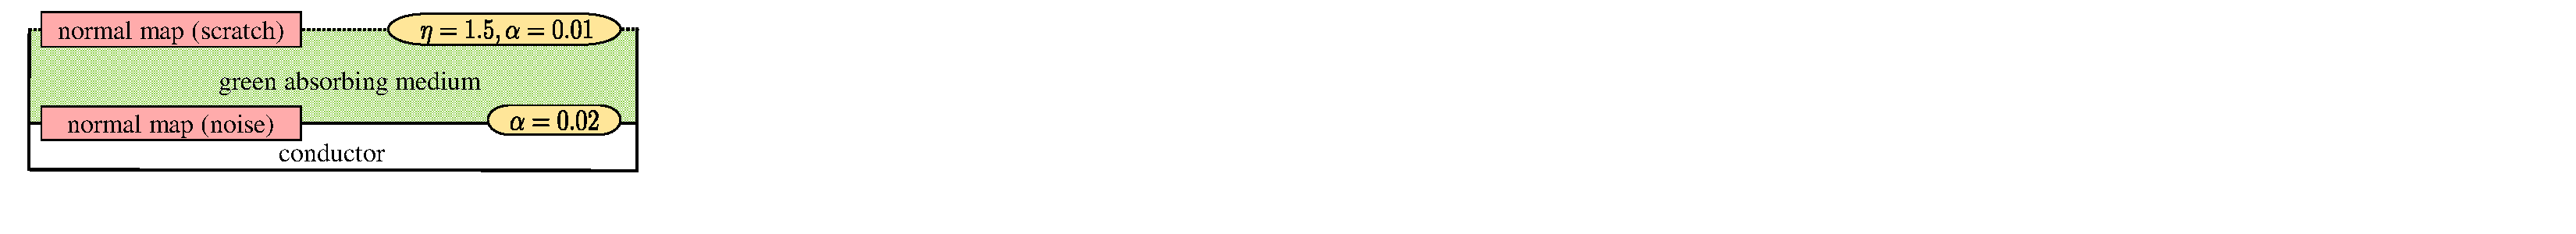
\includegraphics[width=\resLen]{layeredbsdf/teaser/green.pdf} &
		
\includegraphics[width=\resLen]{layeredbsdf/teaser/yellow.pdf} \\
		\textbf{(b2)} & \textbf{(c2)} \\
		
\includegraphics[width=\resLen]{layeredbsdf/teaser/blue.pdf} &
		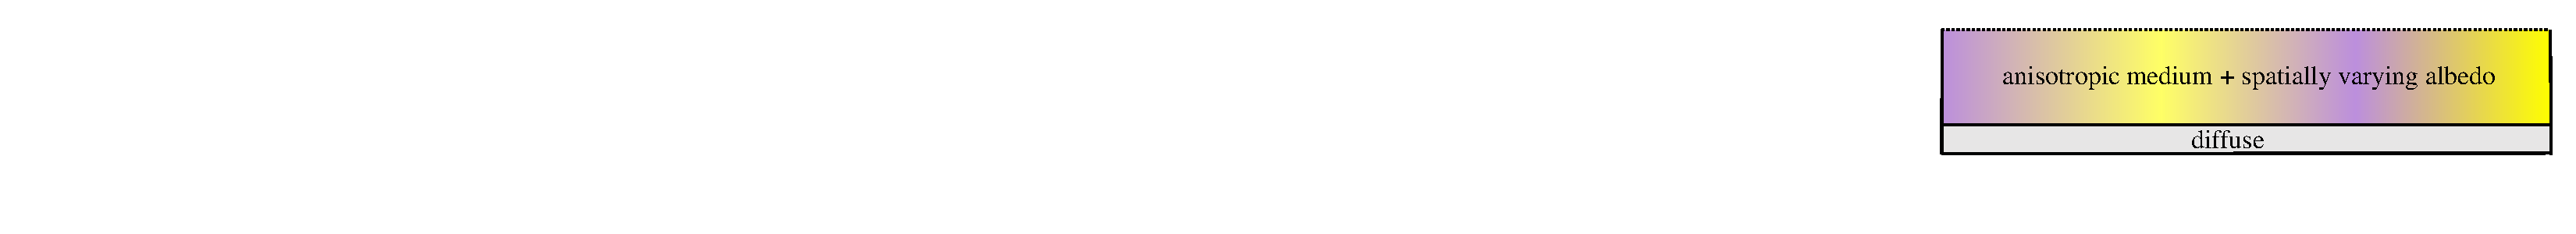
\includegraphics[width=\resLen]{layeredbsdf/teaser/magenta.pdf} \\
		\textbf{(d2)} & \textbf{(e2)}
	\end{tabular}
	\caption[Teaser of LayeredBSDF]{\label{fig:layeredbsdf:teaser}
		We introduce a new BSDF model leveraging an efficient Monte Carlo simulation algorithm applied locally to layered geometries.
		Our model enjoys the flexibility of using arbitrary layer interfaces and internal media and is capable of reproducing a wide variety of appearances.
		This example contains three vases on a tablecloth, all described using our BSDF model (see the insets for layer configurations).
	}
\end{figure}

\section{Introduction}
\label{sec:layeredbsdf:intro}

Physically-based shading models have become mature and commonplace in recent years across a number of rendering applications, within entertainment, architecture, and industrial design. 
However, we are seeing constant progress in the area of material reflection and scattering models, aiming to achieve higher physical realism and to enable more effective material content creation.

Many real world materials are comprised of thin layers with varying compositions. For example, metallic paint is a dielectric coating covering a metallic substrate composed of randomly oriented aluminum flakes; the absorption and scattering properties of the dielectric layer give the material its color and modify its directional scattering properties as well.
Many biological materials (e.g. plant leaves) are also layered, and their appearance is a complex combination of the absorption properties, scattering phase function, air-material interface roughness, and thickness variation.
Different characteristics of such interfaces and volumetric scattering properties can produce richly diverse material appearances from anisotropic highlights to complex textures. Furthermore, detailed layer thickness variations, scratches and bumps on the layer interfaces give these materials additional richness. Accurately understanding and simulating these interactions is therefore key to further progress in the rendering of materials.

\input{tex/layeredbsdf/fig/teaser}

However, explicitly simulating light-layer interactions by modeling the full geometry of these layers would be very expensive and cumbersome. 
The complex and spatially varying interface and internal microgeometries are much too costly to describe and simulate using standard 3D scene modeling tools such as triangle meshes and volumetric grids.
Furthermore, due to the presence of multiple refractive interfaces, it can be very challenging to correctly construct light transport paths that connect light scattering locations to light sources, a key operation in most practical Monte Carlo rendering systems. Cheap approximations to these light transport problems (e.g. ignoring refraction, or composing layers using simple blending) are not sufficient to achieve true realism.

A few techniques have been developed to address this problem. Weidlich and Wilkie \cite{weidlich2007arbitrarily} construct a simple and flexible analytical model. However, significant approximations are necessary; interface roughness is not fully handled for transmission, and no volumetric scattering is supported. The work of Belcour \cite{belcour2018efficient} recently introduced a more advanced approach based on tracking low-order moments of the BSDF lobes; however, it still introduces some approximations and limitations. On the other hand, Jakob et al. \cite{jakob2014comprehensive} (with a recent follow-up \cite{zeltner2018layer}) introduce a solution that is very accurate, but expensive: it represents BSDFs as discretized datasets and relies on expensive Fourier-domain operations on these to implement layer composition and thickness adjustment. This makes free spatial variation of the layer properties prohibitively expensive: a significant limitation in practice.

In this paper, we introduce a new layered BSDF model without the above limitations. Our model provides an accurate, unbiased solution; to our knowledge, it is the only such model.
Unlike previous work, we do not attempt to derive an analytic model for the BSDF lobe shapes. Instead, inside the evaluation and sampling routines of the layered BSDF, we run a Monte Carlo simulation of light transport within flat slabs.
This is substantially faster than explicitly constructing the layer geometry, because no expensive scene ray tracing is required.
Our model computes an accurate solution of the layered light transport problem.
It is based on physical interface and volume scattering models, conserves energy and is reciprocal when possible. It can also be easily integrated into standard Monte Carlo rendering systems.
This requires no precomputation and thus can efficiently handle spatially varying appearances. It also supports the full range of editability of the layer properties, both interface and volumetric, and allows anisotropy in both interface BSDFs and phase functions. In fact, the only limiting assumption of our model is the layer assumption itself.

Our solution is fundamentally more powerful at constructing light transport paths than generic transport algorithms (e.g standard path tracing, bidirectional or Metropolis transport); see Figure \ref{fig:layeredbsdf:equal_time_compare}. We introduce a modified path integral framework for light transport in flat slabs, superior to the standard path formulation in this setting. Because it is based on a product of solid angle instead of area measures, it does not contain the high-variance geometry terms needed in standard algorithms. We introduce two simulation techniques within this formulation: the first is analogous to a forward path tracer with next event estimation through layer boundaries and multiple importance sampling; the second is a fully bidirectional estimator. We show the capabilities of this solution on a number of examples, featuring multiple layers with surface and volumetric scattering. Our examples show spatial variation in all parameters: surface BSDF, volume and phase function parameters, layer thickness and surface normal. See Figure \ref{fig:layeredbsdf:teaser}.


\section{Related Work}
\label{sec:layeredbsdf:related}

\input{tex/layeredbsdf/fig/equal_time_compare}

\subsection{Discretized layered BSDFs}
Previously, a number of BSDF models have been proposed to describe layers with various assumptions on the interface and subsurface scattering.

An early analytical model by Hanrahan and Krueger \cite{hanrahan1993reflection} already supported multiple layers, but only single scattering, and without supporting arbitrary BSDFs at interfaces. They also proposed to add multiple scattering by Monte Carlo simulation, but their simulation approach only considers volume scattering events (as opposed to a combination of volume and rough interface events). Furthermore, it uses binning on the outgoing direction, as opposed to an efficient BSDF evaluation method for a given outgoing direction, which is provided by our approach.
%
%A model by Stam \shortcite{Stam2001} introduces a solution for rendering skin as a layered material consisting of rough dielectric interfaces bounding a volumetric scattering slab. The solution is based on discretization of the BSDF into a directional basis, on which the light transport problem is solved. The model introduced by Jakob~et~al.~\shortcite{Jakob:2014:CFR} can be seen as a significant extension of Stam's discretization approach, working in the Fourier domain. It handles arbitrary layer stacks, supporting subsurface scattering within thin layers using the adding-doubling method, in addition to microfacet rough interfaces. The work of Zeltner extends this approach to anisotropic surface reflectance \shortcite{Zeltner2018}. These models are highly accurate and efficient to render with, once the discretized BSDF has been constructed. However, as the BSDF construction in the discretized basis is relatively expensive, they are best suited for homogeneous BSDFs. A small number of such BSDFs can be spatially blended with varying weights, but this has strict limitations, compared to our support for arbitrary spatial texturing of all parameters.
%
%\subsection{Analytic layered BSDFs}
%The model by Weidlich and Wilkie \shortcite{Weidlich:2007:ALM} takes a different approach. They focus on layers where subsurface scattering is absent (though absorption is allowed), by analytically combining microfacet BSDFs from the interfaces into a single, potentially multi-lobe, microfacet-like BSDF. There are significant approximations in this approach, carefully chosen so that integration (Monte Carlo or otherwise) is never required within a single BSDF query. This makes the model fast and flexible. Another recent model \cite{guo2017rendering} also takes the approach of avoiding Monte Carlo integration during queries, by introducing extended normal distribution functions (ENDFs), analogous to microfacet NDFs but capturing multiple reflection or scattering events. In the most recent work, Belcour \shortcite{Belcour2018} introduced an approach based on tracking low-order moments of the BSDF lobes. This is a very fast and practical solution, but still introduces some approximations and limitations (e.g. no surface or volume anisotropy). In contrast, our method offers unbiased accuracy and even more flexibility, at the cost of some additional computation and variance. \sz{Several previous techniques model light scattering in layered materials like human skin~\cite{Donner:2008:LHR}, but these are focused on lateral light spreading in BSSRDFs, and are orthogonal to our focus on the directional properties of BSDF models.}
%
%\subsection{Microfacet models for interfaces}
%BSDF models based on the microfacet theory are commonly used in computer graphics to capture how light reflects and refracts when interacting with specular surfaces with rough microstructure. The model by Walter~et~al.~\shortcite{Walter:2007:MMR} extends the microfacet model of Cook and Torrance~\shortcite{Cook:1982:RMC} to handle light reflection and transmittance through rough dielectric interfaces, and is currently seen as standard in physically-based rendering. We use this model to describe our layer interfaces.
%
%The microfacet model recently developed by Heitz~et~al.~\shortcite{Heitz:2016:MMB} is capable of capturing interreflections between the facets and better conserves energy. Sch\"ussler \shortcite{Schussler2017} introduced a solution to the energy loss common in normal mapping techniques, caused by a mismatch between the shading and geometric normal. These models (or any future improved microfacet models) could be combined with our approach.
%
%\subsection{Capability comparison}
%In Figure \ref{fig:compare-previous}, we compare the capabilities of our approach to recent work \cite{Zeltner2018,Belcour2018}. We consider three features supported by our approach: surface anisotropy, spatial variation, and volumetric medium anisotropy. Only one of these is supported in the compared systems: spatial variation in Belcour's approach and surface anisotropy in Zeltner's.

%\input{tex/fig/compare_previous}



%\section{Background and overview}
%\label{sec:background}
%
%\input{tex/fig/lobes}
%
%\input{tex/fig/assumption}
%
%In this section, we explicitly state the assumptions of our method, provide background on the standard path formulation of light transport, and provide a quick overview of the rest of the paper.
%
%\subsection{Assumptions}
%
%Although light generally enters and leaves the layer from different locations, we note that when the layers are thin and the lighting is comparably distant, the entrance and departure locations will be close enough to each other. We assume it is acceptable to ignore this displacement, allowing us to describe the light transport in the layers using BSDFs, rather than BSSRDFs (Figure~\ref{fig:thin_layer}).
%
%Furthermore, we assume that the spatial variation of layer properties is slow enough that a BSDF evaluation at a single surface point can locally approximate them as spatially uniform. This is related to the above in assuming that the horizontal spreading of light is small enough to be negligible.
%
%In fact, these are the \emph{only} approximating assumptions of our approach, which otherwise offers unbiased accuracy and full flexibility in setting the layer properties and varying them spatially.
%
%\subsection{Review of Veach's path integral formulation}
%\label{subsec:path_int}
%
%In the Veach formulation of light transport~\shortcite{VeachThesis}, light paths are defined as sequences of vertices connected by segments.
%The value of a light transport integral (for example, but not necessarily limited to, a pixel value) is written as
%%
%\begin{equation}
%I = \int_\Omega f(\bar x) \intd \mu(\bar x),
%\end{equation}
%%
%where $\bar x = (\bx_0, \dots, \bx_k)$ is a path with $k$ segments and $k + 1$ vertices on the surfaces or within the participating media of a scene.
%$\Omega$ is the space of all paths and is defined as the union of $\Omega_k$ for $k \geq 0$, where $\Omega_k$ indicates the set of paths of length $k$.
%Furthermore, $f(\bar x)$ is the path contribution to the integral, and $\mu(\bar x)$ is a special measure on the path space, defined as the product of area measures on the vertices $\bx_i$. The contribution $f(\bar x)$ is a product of vertex terms (normally BSDFs and phase functions) and geometry terms corresponding to path segments. The geometry terms contain the squared distance between the two vertices in the denominator; this is a significant source of variance when trying to connect independently sampled vertices on thin layer configurations.
%
%
%\subsection{Paper overview}
%
%In Section \ref{sec:path-formulation}, we describe our path formulation of layered light transport. Our path integral differs from Veach's formulation in that it is \emph{position-free}. The key idea is that on an infinite flat slab, the horizontal positions of vertices do not matter: it is only the vertical position (depth) of a vertex, and the \emph{directions} between vertices, that are relevant to a light transport integral. The vertices are defined by their depth in the layer, as opposed to a full 3D position, and the segments have variable unit directions.
%
%It is important to note that our position-free formulation is not just a simplified specialization of the standard formulation to the flat slab setting, but in fact a new approach that achieves much superior variance to the standard formulation. The key benefit of this new formulation is that it does not contain the inverse square distance falloff terms that are required between any two vertices with full positional information. The leads to high variance, even in advanced estimators such as bidirectional and Metropolis transport, which in fact perform even worse in this setting than unidirectional; see Figure \ref{fig:validation1} for examples.
%
%In contrast, our approach leads to an efficient estimator based on unidirectional sampling with next event estimation, and an even more efficient bidirectional estimator. The unidirectional performs similarly (though usually not better) in simpler cases, but in challenging cases with sharp and/or anisotropic BSDFs and phase functions, the bidirectional version is clearly more efficient (Figure~\ref{fig:validation1}, bottom). Figure \ref{fig:hemispheres} demonstrates the performance of the estimators through BSDF lobe visualization, also showing a close match to ground truth. In Section \ref{sec:ours}, we describe these two estimators in detail, and also focus on the two additional operations critical for integrating a BSDF into a practical renderer: importance sampling and pdf evaluation.
%
%Finally, we present results in Section \ref{sec:results}, and summarize in Section \ref{sec:conclusion}.
%
%% \subsection{Applying a Monte Carlo estimator}
%% \label{sec:applymc}
%
%% To evaluate the BSDF value $f_l(\omegain, \omegaout)$ for given query directions $\omegain$ and $\omegaout$, we need to evaluate the path integral of Eq.~\eqref{eq:pathintegral} by sampling paths $\bar x$ from some distribution, and weighting the paths by their contribution, divided by their probability densities in the measure $\mu(\bar x)$, i.e. the product of solid angle measures at the internal directions of the path.
%
%% Consider the specific example of $\Omega_3(\omegain, \omegaout)$, i.e. the subspace of paths with three vertices, corresponding to a transmit-reflect-transmit (TRT) configuration.
%% For paths in this subspace, only the directions $\bd_1$ and $\bd_2$ are ``free parameters'' participating in the integration, and the measure is simply the product of solid angle measures at $\bd_1$ and $\bd_2$.
%% This suggests a simple and effective approach for choosing $\bd_1$ and $\bd_2$ (and thus $\bar x$): to importance-sample the top interface BSDF $f_\uparrow$ twice, by using $\omegain$ and $\omegaout$ as the incoming directions, respectively (Figure~\ref{fig:mis_local}-a).
%% Alternatively, one can sample $\bd_1$ and $\bd_2$ by first drawing $\bd_1$ using $f_\uparrow$ (given $\omegain$) and then $\bd_2$ (given $\bd_1$) using $f_\downarrow$ (Figure~\ref{fig:mis_local}-b).
%% This method is more efficient when the bottom interface is close to specular.
%% Both strategies can be combined using MIS to provide a robust sampling scheme for light transport paths $\bar{x} \in \Omega_3(\omegain, \omegaout)$.
%
%% In standard rendering systems, a BSDF sampling procedure commonly returns a ``weight'', defined as the BSDF value in the sampled direction $\bom$, times the cosine term, divided by the probability density (pdf) of picking the direction in the solid angle measure.
%% %\szrem{Need a figure to make this part clearer.}
%% This makes it particularly convenient to compute the path contribution divided by the pdf: simply multiply the two weights returned by importance-sampling $\bd_1$ and $\bd_2$, additionally multiplied by the BSDF at the bottom interface, $f_s(x_2, \bd_1, -\bd_2)$.
%
%% Furthermore, it is clear that there is nothing specific about the TRT mode here, and a minor modification of this approach works for camera and light subpaths of any length. In our concrete implementation, the light subpath has up to one vertex, while the camera subpath can have any length.

\section{Position-Free Path Formulation}
\label{sec:layeredbsdf:pathformulation}

In this section, we theoretically define the value of a layered BSDF due to a given layer stacking, for given query directions $\omegain$ and $\omegaout$, as a path integral. Given such a definition, any Monte Carlo method can be used to evaluate the BSDF by randomly sampling paths, evaluating their contributions and dividing by the corresponding probability density values.

\subsection{Notation}

We will use the notation $\cos \bom$ to denote the $z$-component of the unit vector $\bom$. We will also use $\ind(x)$ to denote an indicator function, returning 1 if the boolean condition $x$ is true and 0 if false. A bold font is used to denote unit vectors (directions) on $\Sph$. Please refer to Table \ref{tab:layeredbsdf:notation} for the notation used in this section.

\input{tex/layeredbsdf/tab/notation}

\subsection{Position-free path integral}

To develop the theory, we will first assume a single infinite flat slab with a BSDF $f_\uparrow$ on the top interface and a BSDF $f_\downarrow$ on the bottom interface, combined with a homogeneous scattering volume inside the slab to produce a resulting layered BSDF. The volumetric medium is defined by a phase function $f_p$, scattering coefficient $\sigma_s$ and extinction coefficient $\sigma_t$; we will use the notation $\hat f_p = \sigma_s f_p$.

For simplicity, we will drop the depth dependence of the volume parameters (though they could vary) and we will assume constant scattering / extinction coefficients, though they can vary with direction for fully anisotropic phase functions, which we also support. We will further assume that the slab has unit thickness; the formulation can be easily adjusted for any thickness.

A {\bf vertex} $z_i \in [0, 1]$ is a single real number indicating the depth within the layer. A value of 0 or 1 indicates a surface reflection or refraction event on the bottom or top interface, respectively. Fractional values indicate volume scattering events at the specified depth. Note again that the horizontal positions of vertices on the infinite flat interfaces are not needed.

A {\bf direction} $\bd_i$ is a unit vector on $\Sph$ denoting the light flow between vertices. In our convention (inherited from Veach), 
the vectors point in the direction of light flow (i.e. from light source to camera), and the vertex/direction indexing follows this as well.

A {\bf light path} $\bar x$ is a sequence of directions and vertices: $\bar x = (\bd_0,\ z_1,\ \bd_1,\ \dots,\ z_k,\ \bd_k)$.
The first and last directions are aligned with the input and output directions of the layered BSDF query, i.e. $\bd_0 = -\omegain$ and $\bd_k = \omegaout$. In contrast to Veach's formulation, the path interleaves directions with vertices, and the two ends of the path are defined by directions (not vertices). See Figure \ref{fig:layeredbsdf:paths} for some example paths.

\input{tex/layeredbsdf/fig/paths}

The {\bf path contribution} $f(\bar x)$ of a light path is the product of vertex terms $v_i$ (on each vertex) and segment terms $s_i$ (on all internal segments):
\begin{equation}
	f(\bar x) = v_1 s_1 v_2 s_2 \dots s_{k-1} v_k.
\end{equation}
The vertex term consists of the BSDF or phase function value:
\begin{equation}
\label{eqn:vtx_contrib}
v_i = v(z_i, -\bd_{i - 1}, \bd_i)
= \begin{cases}
	f_\uparrow(-\bd_{i-1}, \bd_i)   & \mbox{  if  } z_i = 0,\\
	f_\downarrow(-\bd_{i-1}, \bd_i) & \mbox{  if  } z_i = 1,\\
  	\hat{f}_p(-\bd_{i-1}, \bd_i)    & \mbox{  if  } 0 < z_i < 1.
\end{cases}
\end{equation}
Define the transfer term $\tau(z_1, z_2, \bom)$ as follows:
\begin{equation}
\tau(z, z', \bom) := \exp \left( \frac{-\sigma_t |z' - z|}{|\cos \bom|} \right) \cdot \ind \left( \frac{z' - z}{\cos \bom} > 0 \right).
\end{equation}
The purpose of the exponential term is to compute the transmittance when going from depth $z$ to $z'$ following direction $\bom$.
The indicator term checks the validity of the configuration (i.e. if the direction points up, then $z'$ should be greater than $z$, and vice versa). The segment term for internal segments can now be defined as:
\begin{equation}
\label{eqn:seg_contrib}
s_i = s(z_i, z_{i + 1}, \bd_i) := \tau(z_i, z_{i+1}, \bd_i) \cdot |\cos \bd_i|^{\alpha_i},
\end{equation}
where
\begin{equation}
\label{eqn:seg_contrib_cosine}
\alpha_i = \ind(z_i \in \{0,1\}) + \ind(z_{i + 1} \in \{0,1\}) - 1.
\end{equation}
This definition encapsulates the subtle behavior of cosine terms along the path segments.
For a detailed derivation, please refer to Appendix \ref{sec:layeredbsdf:derivation}.

The {\bf path space} $\Omega(\omegain, \omegaout)$ is the set of all paths of one or more vertices, such that the first direction of the path is equal to $-\omegain$ and the last to $\omegaout$. It can be seen as the union of the spaces of such paths of all lengths $k \geq 1$, that is, $\Omega = \cup_{k \geq 1} \Omega_k$.

The {\bf path space measure} $\mu(\bar x)$ is a product of solid angle measures $\sigma$ on the internal directions of the path, times the product of line measures $\lambda$ on volumetric scattering vertices.
That is, for a $k$-vertex path,
\begin{equation}
\mu(\bar x) = \prod_{i=1}^{k-1} \sigma(\bd_i) \cdot \prod_{i \in V(\bar x)} \lambda(z_i).
\end{equation}
Here $V(\bar x)$ is the set of indices of volumetric vertices on $\bar x$, and $\lambda$ is the line measure (i.e. standard Lebesgue measure on the real numbers).

Finally, we can define the {\bf layered BSDF value} $f_l(\omegain, \omegaout)$ as an integral over the set of paths $\Omega(\omegain, \omegaout)$:
\begin{equation}
\label{eq:pathintegral}
	f_l(\omegain, \omegaout) = \int_{\Omega(\omegain, \omegaout)} f(\bar x) \intd \mu(\bar x).
\end{equation}
As usual, any Monte Carlo method can be used to compute this integral. As long as the probability density $p(\bar x)$ with respect to measure $\mu(\bar x)$ of generated sample paths is known, we simply average a number of samples of the form $f(\bar x) / p(\bar x)$.


\subsection{Derivation}

Here we sketch the derivation of the path formulation.
Like in Veach's version (and its volumetric extension), the derivation proceeds by recursively expanding the surface and volume rendering equation (the latter also commonly known as the radiative transfer equation). Denote the surface radiance by $L_s(z, \bom)$ (for $z \in \{0, 1\}$) and the volume radiance $L_v(z, \bom)$ (for $z \in [0,1]$).

The volume radiance will satisfy the standard radiative transfer equation, specialized to our position-free setting:
\begin{equation}
\label{eq:IRTE}
L_v(z, \bom) = S(z, \bom) + 
\int_0^1 \frac{\tau(z', z, \bom)}{|\cos\bom|} \, \, \int_{\Sph} \hat f_p(\bom', \bom) \, L_v(z', \bom') \,\intd \bom' \intd z',
\end{equation}
where the source term $S(z, \bom)$ gives illumination from the boundary of the slab:
\begin{equation}
S(z, \bom) = \tau(0, z, \bom) L_s(0, \bom) \ + \ \tau(1, z, \bom) L_s(1, \bom).
\end{equation}
Notice that, although the source term has two components, only one of them will be non-zero for any given query.
This formulation is valid even with no scattering within the layer, in which case $\hat f_p = 0$ and the second term of Eq. \eqref{eq:IRTE} vanishes.
Further, the $1/|\cos\bom|$ factor is due to a change of variable (from free-flight distance to depth). For more details, please refer to Appendix \ref{sec:layeredbsdf:derivation}.

The surface radiance $L_s(z, \bom)$ satisfies the standard rendering equation:
\begin{equation}
\label{eq:RE}
L_s(z, \bom) = \int_{\Sph} f_s(z, \bom, \bom') \ |\cos \bom'| \ L_s^i(z, \bom') \intd \sigma(\bom'),
\end{equation}
where $L_s^i(z, \bom')$ is the incoming surface radiance. In case the incoming radiance query points back into the layer, we have
\begin{equation}
\label{eq:incoming}
L_s^i(z, \bom) = L_v(z, -\bom).
\end{equation}
The BSDF value is defined as the radiance leaving the surface in direction $\omegaout$, under unit irradiance from a directional light in direction $\omegain$. This is equivalent to evaluating $L_s(1, \omegaout)$ under the boundary condition
\begin{equation}
	\label{eq:bound}
	L_s^i(z, \bom) = \frac{\delta(\bom - \omegain)}{|\cos \omegain|}.
\end{equation}
One can easily check that the irradiance under this illumination is unit. Thus the incoming surface radiance $L^i_s$ is given by Eq. \eqref{eq:bound} when $\bom$ points out of the layer and Eq. \eqref{eq:incoming} when it points back into the layer.

The path formulation can now be obtained by recursively expanding the desired value $L_s(1, \omegaout)$ using the above equations for $L_s$ and $L_v$, terminating the paths using the boundary condition. Note that:
\begin{itemize}
	\item Each recursive expansion of Eqs. \eqref{eq:IRTE} or \eqref{eq:RE} will contribute an $\hat f_p$ or $f_s$ term, respectively, to the path vertex.
	\item Each volumetric segment will introduce a $\tau(z, z', \bom)$ term, whether the first or second term in Eq. \eqref{eq:IRTE} is taken.
	\item{Expanding the rendering equation contributes a cosine term to the \emph{next} segment, while expanding the radiative transfer equation contributes a 1/cosine term to the \emph{previous} segment. A combination of these contributions explains the $\alpha_i$ term above.}
	\item The last surface cosine is canceled out when using the boundary condition, due to the denominator cosine in Eq. \eqref{eq:bound}.
\end{itemize}


\subsection{Normal mapping}

An important feature of our method is the mapping of normals of the layer interfaces, introducing mismatches between geometric (flat) normals and shading (mapped) normals. The definition of the segment term (Eq. \eqref{eqn:seg_contrib}) changes with the presence of shading normals. Precisely, it becomes
\begin{equation}
s_i = \tau(z_i, z_{i+1}, \bd_i) \ \frac{|\langle \bn(z_i), \bd_i \rangle| \ |\langle \bn(z_{i + 1}), \bd_i \rangle|}{|\cos \bd_i|},
\end{equation}
where $\bn(z)$ denotes the local shading normal at $z$ (for $z \in \{0, 1\}$). This term is no longer symmetric, which implies that BSDFs with mapped normals will in general not be reciprocal. When sampling paths from the light, it is important to handle such BSDF using the correction term introduced by Veach \cite{veach1997robust} (Eq. 5.19).


\subsection{Note about reciprocity}

Our layered BSDF will be reciprocal whenever the path contribution $f(\bar x)$ is symmetric with respect to the reversal of the path. Assuming normal mapping is not used, the segment term $s_i$ will be symmetric, so the reciprocity boils down to the symmetry of the vertex terms $v_i$. This will certainly hold if all phase functions and BSDFs are reciprocal.

Note, however, that crossing an interface between regions of different index of refraction (whether smooth or rough) is not reciprocal in the usual sense. Instead, a physical refractive BSDF should obey a modified reciprocity relation $f_s(\omegain, \omegaout) = \eta_o^2 / \eta_i^2 \cdot f_s(\omegaout, \omegain)$ \cite{walter2007microfacet}, where $\eta_i$ and $\eta_o$ are the refractive indices of the corresponding media. In the common case where the layered BSDF's incoming and outgoing directions are both assumed to be in air, the final layered BSDF will still be reciprocal, because there will be an equal number of $\eta^2$ and $1/\eta^2$ terms along the path for each medium with index $\eta$.


\subsection{Multiple slabs}
\label{subsec:multi_layer}

Finally, we support extending the framework to multiple slabs. This is relatively straightforward theoretically, and simply requires explicitly keeping track of the interface or volume that a vertex/segment belongs to. We also need to modify the transfer term $\tau(z,z'\bom)$ to return zero in cases when the segment crosses an internal interface.

Another option to obtain a multi-layer BSDF is by recursively nesting the BSDFs. To construct the layered BSDF due to a layer stacking of $n$ slabs, we define the layered BSDF due to the stacking of the bottom $n-1$ slabs, and use this BSDF as the bottom interface's BSDF in adding the top layer according to the above theory. We have found that this approach works in practice, but its performance is worse than the explicit implementation above.



\section{Our Estimators}
\label{sec:layeredbsdf:ours}

We now describe our specific layered BSDF method,
by presenting our Monte-Carlo solutions to enable the three key operations needed to fully define a BSDF model:
sampling (\S\ref{subsec:ours_sample}), evaluation (\S\ref{subsec:ours_eval}) and pdf computation (\S\ref{subsec:ours_pdf}).
Sampling produces the outgoing direction $\omegaout$ given the incoming one $\omegain$ (or the reverse), while evaluation answers the BSDF query for given $\omegain$ and $\omegaout$. Note that the values returned from sampling, evaluation and pdf procedures are themselves stochastic, and are equal to the true BSDF value, pdf value or sampling weight only in expectation. Stochastic evaluation was also used in some recent BSDF models \cite{heitz2016multiple}. 

Multiple importance sampling (MIS) is commonly used to combine multiple techniques to produce a given path, and key to obtaining low-noise results under complex lighting conditions. This technique typically uses the sampling pdfs of the techniques being combined to derive the weights, which requires the pdf values of the layered BSDFs. We introduce two solutions: an unbiased solution for estimating the exact pdf values in expectation, as well as a fast and approximate version which we demonstrate is sufficient for MIS (\S\ref{subsec:ours_pdf}). In a supplementary document, we show that the estimators are still unbiased in the presence of approximate pdfs for MIS weighting and stochastic evaluation of both weights and function values.

\subsection{BSDF sampling}
\label{subsec:ours_sample}

Sampling a BSDF is the problem of drawing the outgoing direction $\omegaout$ given the incoming one $\omegain$ (or the reverse), with a pdf proportional, exactly or approximately, to the value $f_l(\omegain, \omegaout)$ (times the cosine term, if possible).
This is straightforward: we draw $\omegaout$ simply by following the stochastic process given by light interacting with the layered configuration.
That is, we utilize a pure forward path tracing process that starts with a ray with direction $-\omegain$ and explicitly simulates interactions between the ray and the layer's interfaces and internal media by sampling the corresponding BSDFs and phase functions, accumulating a throughput value along the way.
When the ray eventually leaves the layer, its direction gives $\omegaout$ and the throughput of the full light transport path gives the stochastic sample weight. Formally, this weight is an estimate of the BSDF value, times the exitant cosine direction, divided by the sampling pdf in solid angle measure.

Although this simulation is analogous to standard Monte Carlo path tracing, it is usually much more efficient than tracing paths in the global scene thanks to the simplicity of the flat slab configuration (under which ray tracing becomes simple numerical computation, not requiring any acceleration structures).

\subsection{BSDF evaluation}
\label{subsec:ours_eval}

To evaluate our BSDF $f_l$ at given incoming and outgoing directions $\omegain$ and $\omegaout$, we introduce two Monte Carlo based methods to evaluate the path integral from Eq. \eqref{eq:pathintegral}.
The first one (\S\ref{sssec:ours_unidir}) is analogous to a unidirectional path tracer with next-event estimation (NEE), while the second (\S\ref{sssec:ours_bidir}) uses a bidirectional scheme.

\subsubsection{Unidirectional simulation}
\label{sssec:ours_unidir}

In standard path tracing, a shading point would be directly connected to a light source in a process often called \emph{direct illumination} or \emph{next event estimation} (NEE), which is crucial for low-variance rendering. In an analogy to this technique, consider a shading point inside a single layer slab (whether on the bottom interface or a scattering point within the medium). We would like to create a path ending with $\omegain$, intuitively connecting it to an external directional light source with direction $\omegain$. However, direct connection between the shading point and the desired external direction is usually invalid due to the layer's top refractive interface.

To address this problem, we introduce our NEE scheme that directly connects scattering events across potentially rough refractive interfaces.
Assume without loss of generality that our path tracing starts with direction $\omegaout$.
At each scattering event, we need to find a direction $\omegain'$ so that $\omegain \to \omegain'$ follows the BSDF at the interface.
To this end, we draw $\omegain'$ by sampling the interface BSDF backwards, given $\omegain$.
Finally, we simply multiply the accumulated throughput by the weight returned from the sampling routine, and the BSDF (or phase function) value at the scattering event.

Furthermore, this NEE connection can be combined with a path continuation (by sampling the phase function or interface BSDF), using MIS for the weighting. This is analogous to the MIS direct illumination used in many practical path tracers, with the difference that the path can cross a refractive boundary. Note the distinction between this \emph{local} MIS, and the \emph{global} MIS used by the scene-level transport algorithm (a standard path tracer in our results). An illustration of these two techniques, applied to a transmit-reflect-transmit (TRT) configuration, can be found in Figure \ref{fig:layeredbsdf:mc_estimators}-ab.

\input{tex/layeredbsdf/fig/mc_estimators}

Previous work on next-event estimation in scattering volumes through refractive interfaces \cite{walter2009single,koerner2016subdivision} is related to our scheme, but focuses on arbitrary geometries, which is not necessary in the flat layer setting.

Extending this NEE scheme to cross multiple layer interfaces is somewhat tedious to implement, as care must be taken not to double-count light paths. We instead use the recursive nesting approach to multiple layers (\S\ref{subsec:multi_layer}) when using the unidirectional estimator, which handles these issues automatically.


\subsubsection{Bidirectional simulation}
\label{sssec:ours_bidir}

Although our unidirectional solution works well in many cases, we introduce a new bidirectional approach that performs even better.
Our approach is conceptually similar to bidirectional path tracing (BDPT) but is technically different in several ways due to our position-free path formulation.

Given the incoming and outgoing directions $\omegain$ and $\omegaout$, consider two light transport paths, generated from the light and camera, respectively.
\begin{equation}
\begin{aligned}
\bar{x}_i &= (\bd_0, z_1, \bd_1, \ldots, z_s) \\
\bar{x}_o &= (\bd'_0, z'_1, \bd'_1, \ldots, z_t'),
\end{aligned}
\end{equation}
where $\bd_0 = -\omegain$ and $\bd'_0 = -\omegaout$ (Figure \ref{fig:layeredbsdf:mc_estimators}-c).
Now we can construct a full light path $\bar{y}_{s, t}$ connecting the $s$-th vertex in $\bar{x}_i$ and the $t$-th vertex in $\bar{x}_o$ (assuming the connection between $z_s$ and $z'_t$ does not cross any layer boundary):
\begin{equation}
\bar{y}_{s, t} = (\bd_0, \ldots, z_{s - 1}, \bd_{s - 1}, z_s, \tilde{\bd}, z'_t, -\bd'_{t - 1}, z'_{t - 1}, \ldots, -\bd'_0).
\end{equation}
Unlike traditional BDPT, where the connection term between two given subpaths endpoints is fixed, there exists infinitely many valid directions $\tilde{\bd}$ connecting $z_s$ and $z'_t$ in our case, which gives us freedom to importance-sample the direction. In practice, we choose $\tilde{\bd}$ in two ways by sampling additional directions $\bd_s$ and $\bd'_t$ by extending the two subpaths with an extra importance sampling step. We set $\tilde{\bd}$ to $\bd_s$ and $-\bd'_t$ respectively. This yields two light paths $\bar{y}^{(0)}_{s, t}$ and $\bar{y}^{(1)}_{s, t}$ (Figure \ref{fig:layeredbsdf:mc_estimators}-de), thus providing two samples of the path integral.
Denote the extended subpaths by
\begin{align}
\bar{x}_i^+ &:= (\bd_0, z_1, \bd_1, \ldots, z_s, \bd_s),\\
\bar{x}_o^+ &:= (\bd'_0, z'_1, \bd'_1, \ldots, z'_t, \bd'_t),
\end{align}
and let $\bar{x}^*$ denote the adjoint (reversed) version of a light path $\bar{x}$, e.g., \\$\bar{x}_o^{+*} = (-\bd'_t, z'_t, -\bd'_{t - 1}, \ldots, z'_1, -\bd'_0)$.

Let $v(z, \bom, \bom')$ and $s(z, z', \bom)$ be the vertex and segment contributions defined in eqs. \eqref{eqn:vtx_contrib} and \eqref{eqn:seg_contrib}.
We can easily verify that
\begin{align}
f(\bar{y}_{s,t}^{(0)}) &= f(\bar{x}_i^+) \, f(\bar{x}_o^*) \, s(z_s, z'_t, \bd_s) \, v(z'_t, -\bd_s, -\bd'_{t - 1}),\\
f(\bar{y}_{s,t}^{(1)}) &= f(\bar{x}_i) \, f(\bar{x}_o^{+*}) \, v(z_s, -\bd_{s - 1}, -\bd'_t) \, s(z_s, z'_t, -\bd'_t).
\end{align}
It follows that the two Monte Carlo estimates will be:
\begin{align}
\label{eqn:bidir_estimate_i}
\frac{f(\bar{y}^{(0)}_{s, t})}{p(\bar{y}^{(0)}_{s, t})} &=
\frac{f(\bar{x}_i^+)}{p(\bar{x}_i^+)}
\frac{f(\bar{x}_o^*)}{p(\bar{x}_o)}
\, s(z_s, z'_t, \bd_s) \, v(z'_t, -\bd_s, -\bd'_{t - 1})\\
%
\label{eqn:bidir_estimate_j}
\frac{f(\bar{y}^{(1)}_{s, t})}{p(\bar{y}^{(1)}_{s, t})} &=
\frac{f(\bar{x}_i)}{p(\bar{x}_i)}
\frac{f(\bar{x}_o^{+*})}{p(\bar{x}_o^+)}
\, v(z_s, \bd_{s - 1}, \bd'_t) \, s(z_s, z'_t, -\bd'_t),
\end{align}
Note that in general $f(\bar x_o) \neq f(\bar x_o^*)$ and $f(\bar x_o^+) \neq f(\bar x_o^{+*})$ due to non-reciprocal operations such as shading normals; care must be taken to compute correct throughputs of light subpaths, as detailed in Chapter 5 of Veach \cite{veach1997robust}.

The above discussion assumed a single light and single camera subpath. In practice, we combine all prefixes of the sampled subpaths. In particular, we sample subpaths of length $n_i$ and $n_o$ from the light and camera respectively (the lengths are chosen through Russian roulette):
\begin{equation}
\begin{aligned}
\bar{x}_i &= (\bd_0, z_1, \bd_1, \ldots, z_{n_i}, \bd_{n_i}),\\
\bar{x}_o &= (\bd'_0, z'_1, \bd'_1, \ldots, z'_{n_o}, \bd'_{n_o}).
\end{aligned}
\end{equation}
For all $s$ and $t$ combinations, Eqs. \eqref{eqn:bidir_estimate_i} and \eqref{eqn:bidir_estimate_j} provide $2 n_i n_o$ estimators of $f_l(\omegain, \omegaout)$.
Combining them using MIS gives us our bidirectional estimator for paths of length 2 or more vertices. We handle single vertex paths separately. The details of MIS weighting are discussed in the supplementary document.


\subsection{Pdf estimation}
\label{subsec:ours_pdf}

Another important operation for practical BSDF models is to evaluate the probability density for sampling provided incoming and outgoing directions.
That is, to evaluate $p(\omegaout \;|\; \omegain)$, the probability density of $\omegaout$ given $\omegain$ (assuming that the sampling process draws $\omegaout$ and fixes $\omegain$).
This operator is used for weight computation in multiple importance sampling (using balance or power heuristics), a crucial technique for generating low-noise results using scene-level Monte Carlo rendering techniques. Note that this pdf is in the solid angle measure; it is a marginal pdf distinct from the path pdf $p(\bar x)$.

Although $p(\omegaout \;|\; \omegain)$ is usually easily available for traditional analytical BSDFs, no closed-form pdf exists in our case. Instead, the pdf evaluation has comparable form to the BSDF evaluation itself. It can be expressed using another position-free path integral:
\begin{equation}
\label{eqn:ours_pdf}
p(\omegaout \;|\; \omegain) = \int_{\Omega(\omegain, \omegaout)} \mathcal{P}(\bar{x}) \intd\mu(\bar{x}),
\end{equation}
where
\begin{equation}
\mathcal{P}(\bar{x}) := \left(\prod_{j = 1}^k p(\bd_j \;|\; z_j, \bd_{j - 1})\right) \left(\prod_{j = 1}^{k - 1} p(z_{j + 1} \;|\; z_j, \bd_{j - 1})\right),
\end{equation}
with $k$ denoting the number of vertices in $\bar{x}$. Note that $\bd_k = \omegaout$.

We introduce two nondeterministic methods, an unbiased and a fast approximate approach, to estimate $p(\omegaout \;|\; \omegain)$.
These operations are not used in standard Monte Carlo light transport and are new, to our knowledge.
In practice, the approximate approach can be used when exact estimations are unnecessary (as is the case for a global path tracer with MIS, which we use for our results).
Note that the estimated $p(\omegaout \;|\; \omegain)$ is only ever used for MIS weight computation.
We never use approximate path pdfs for Monte Carlo estimates, as this would introduce bias.
Our BSDF value estimators directly return path throughput with accurate pdf factored in.

\subsubsection{Unbiased pdf estimation}
\label{sssec:ours_pdf_unbiased}

Both our unidirectional and bidirectional Monte Carlo estimators introduced in \S\ref{subsec:ours_eval} can be adapted to estimate the path integral in Eq. \eqref{eqn:ours_pdf} in an unbiased manner.
For instance, the estimators given by Eqs. \eqref{eqn:bidir_estimate_i} and \eqref{eqn:bidir_estimate_j} simply require a replacement of $f$ by $\mathcal P$, and become:
\begin{align}
	\label{eqn:bidir_pdf_i}
	\frac{\mathcal{P}(\bar{y}^{(0)}_{s, t})}{p(\bar{y}^{(0)}_{s, t})} &= \frac{\mathcal{P}(\bar{x}_o^*)}{p(\bar{x}_o)}
	 p( \bd_s \;|\; z'_t, -\bd'_{t - 1}) \, p(z'_t \;|\; z_s, \bd_s),\\
	\label{eqn:bidir_pdf_j}
	\frac{\mathcal{P}(\bar{y}^{(1)}_{s, t})}{p(\bar{y}^{(1)}_{s, t})} &= \frac{\mathcal{P}(\bar{x}_o^{+*})}{p(\bar{x}_o^+)}
	 p( \bd'_t \;|\; z_s, \bd_{s - 1}) \, p(z_s \;|\; z'_t, \bd'_t ).
\end{align}
Note that some cancellation occurs because $p(x_i) = \mathcal P(x_i)$, but in general $p(x_o) \neq \mathcal P(x_o^*)$.

When jointly estimating the path integrals for the BSDF value \eqref{eq:pathintegral} and the conditional probability \eqref{eqn:ours_pdf}, the light transport paths $\bar{x}$ need to be sampled \emph{independently} to ensure unbiasedness.
Please refer to the supplemental document for a proof.

\subsubsection{Approximate pdf estimation}
\label{sssec:ours_pdf_approx}
%
Although the adapted estimators defined in \ref{sssec:ours_pdf_unbiased} provide unbiased pdf estimations, they introduce computational overhead comparable to the BSDF evaluation itself.
Thus, for applications where unbiased pdfs are unnecessary, we introduce an approximation to accelerate the pdf estimation process. The key idea is to only consider short paths reflecting/refracting from interfaces, as these events have the largest effect on the pdf lobe shape, and add a constant (Lambertian) term to approximate the effect of volume scattering and longer paths.

In practice, we run Monte Carlo simulation on a simplified layer configuration where all volumetric media are removed.
We further limit the maximal number of vertices on the light paths to $(2L + 1)$ when $\omegain \cdot \omegaout > 0$ (i.e., $f_l(\omegain, \omegaout)$ captures reflection) and $(L + 1)$ when $\omegain \cdot \omegaout < 0$ (i.e., $f_l(\omegain, \omegaout)$ captures transmission) where $L$ denotes the number of layers.
Lastly, we add a small constant term to the estimation result. The exact scaling of this term is not important for MIS weighting (as it will be overwhelmed by the pdfs of sharply peaked lobes) and we found setting it to 0.1 works well.

\input{tex/layeredbsdf/fig/validate_pdf}

See Figure \ref{fig:layeredbsdf:validate_pdf} for validation of the above pdf approaches against ground truth, and Figure \ref{fig:layeredbsdf:mis} for a comparison between renderings using the unbiased and approximated pdf estimation results. 
All the other results in our paper are using approximated PDF for MIS. Unbiased PDF is much slower, because it requires long light paths, and has to be computed twice per shading event.

\input{tex/layeredbsdf/fig/mis}




\section{Applications and Results}
\label{sec:results}

In this section, we first provide experimental validations (\S\ref{subsec:res_validation}) and then showcase our method on a number of applications and demonstrate its effectiveness (\S\ref{subsec:res_main}).
All the renderings are generated using the Mitsuba physically based renderer \cite{jakob2010mitsuba} with our layered model implemented as a BSDF plugin.
Please see the accompanying video for animated versions of several results.

All the multi-layer results in the paper use our bidirectional estimator with the explicit implementation (although our BSDF plugin also supports nesting BSDFs).
This is because the former runs faster, as seen in Figure \ref{fig:layeredbsdf:result_multilayer}-(c).

\subsection{Validations}
\label{subsec:res_validation}

\subsubsection{Cross validation}
In Figures \ref{fig:layeredbsdf:lobes} and \ref{fig:layeredbsdf:validate_pdf} as well as the supplemental material, we cross-validate our Monte Carlo estimators depicted in \S\ref{subsec:ours_eval} by comparing our estimated BSDFs/pdfs to references generated using forward sampling (\S\ref{subsec:ours_sample}) and binning. Notice that the sampling procedure is a straightforward process that requires none of the complexity introduced by our path formulation and estimators.

\subsubsection{White furnace tests}
We conducted a few ``white furnace tests'' to demonstrate the energy conservation of our layered BSDFs (Figure \ref{fig:layeredbsdf:white_test}).
For all these examples, the BSDFs are constructed such that no energy is lost due to light-layer interactions.
Under constant lighting (where identical amount of light comes from all directions), the object becomes invisible, demonstrating that our layered BSDFs indeed conserve energy properly.

\input{tex/layeredbsdf/fig/white_test}


\subsection{Main Results}
\label{subsec:res_main}

\subsubsection{Application: Coating thickness/normal variation}

Figure \ref{fig:layeredbsdf:globe} shows renderings of a globe with a dielectric coating on top of a metallic substrate.
In this example, both interfaces are colorless and the layer medium has a blue tint.
In Figure \ref{fig:layeredbsdf:globe}-(a), both interfaces are smooth, creating two overlapped reflections of the environment map with different amounts of blur.
In Figure \ref{fig:layeredbsdf:globe}-(b), the top interface of the globe is smooth, leading to one clear reflection.
On the bottom (metallic) interface, we use a detailed height field to drive the normal variation as well as the medium thickness.
The high-frequency variation of normal direction has resulted in detailed highlights on the bottom surface.
Further, due to varying amounts of attenuation at different thickness, these highlights exhibit different colors: reflections from greater depths become darker and more saturated. 
In Figure \ref{fig:layeredbsdf:globe}-(c), the height variation is instead applied to the top dielectric interface, causing the clear reflection of the environment to be replaced by a blurred one.
Further, since the areas under the continents now have larger thickness, their colors become more saturated.
Our layered BSDF model is capable of producing all these appearances using a simple set of parameters (thickness, roughness and medium absorption) in conjunction with spatial variation.

\input{tex/layeredbsdf/fig/globe} 

\subsubsection{Application: Complex thin sheet transmission}

Our physically based BSDF is capable of accurately modeling not only reflection but also transmission.
Figure \ref{fig:layeredbsdf:zhaoyun} contains an example flat surface rendered with our layered BSDF under varying illuminations.
This model involves dielectric interfaces with spatially varying roughnesses and a normal map applied to the front surface.
The optical thickness at each location is obtained by multiplying a base density, which varies across the color channels, by the geometric height field matching the normal map.
In other words, the optical densities (mean free paths) are spectrally varying, which results in subtle color variations across the surface (especially for transmitted light), a phenomenon that would be challenging to model accurately using existing BSDF models. Note again that all of these effects come from the BSDF model, as the scene geometry is a simple flat polygon.

\input{tex/layeredbsdf/fig/zhaoyun}
\input{tex/layeredbsdf/fig/magnifier}

Figure \ref{fig:layeredbsdf:magnifier} shows renderings of a magnifying lens filled with scattering media with spatially varying thickness (which captures the shape of real convex lens). Note that the scene geometry is still just a flat surface.
When coupled with different phase functions (Henyey-Greenstein and von-Mises-Fisher, with different forward scattering parameters), a range of spatially varying and physically plausible blurring effects can be achieved.

Please see the supplemental images and video for more variations with similar configurations.

\subsubsection{Application: Anisotropic layer media for fabrics}

Our layered BSDF allows any phase functions within volumetric scattering layers, including anisotropic microflake phase functions \cite{jakob2010radiative,zhao2011building,heitz2015sggx} capable of representing fabrics.
Figure \ref{fig:layeredbsdf:cloth} shows three fabrics modeled using our model with ``null'' top and bottom interfaces (ones that allows light to travel through without reflecting or refracting it) and anisotropic layer media with spatially varying albedo and flake orientations (the optical density does not vary in these examples, though it could).
The satin weave shows well aligned yarns have created smooth and strongly anisotropic highlights. The twill pattern has warp and weft yarns in different colors, leading to dual colored highlights. The velvet exhibits strong grazing-angle highlights, an effect that is challenging to model using traditional BSDF models. Our model successfully captures all the diverse appearances from all three fabrics and produces convincing impressions of these materials.

\input{tex/layeredbsdf/fig/cloth}

Figure~\ref{fig:layeredbsdf:cloth_compare} shows a fabric rendered using fiber orientation data acquired by micro-CT imaging \cite{zhao2011building}. Our rendering uses a fiber orientation map derived from the full data, and matches the full volumetric simulation fairly closely, while being 40 times faster. The speedup is because ours is still a flat BSDF model with parameter mapping, as opposed to full volumetric tracing that requires expensive ray marching through massive data.

\input{tex/layeredbsdf/fig/cloth_compare}

\subsubsection{Application: Multiple layers}

Lastly, in Figure \ref{fig:layeredbsdf:kettle}, we show rendered results of a kettle with varying layer configurations.
In column (a), the material has a single transparent water layer with a dielectric interface on the top and a metallic surface on the bottom.
Both interfaces are normal mapped to capture the water drops and the scratches, respectively.
In column (b), the material shares the same bottom surface as in (a) but has a smooth top interface and a translucent coating layer with spatially varying optical thickness and albedo, making only part of the bottom surface directly visible.
Lastly, in column (c), the material has a dual-layer configuration by stacking the layers from (a) on top of that from (b).
Our method offers the flexibility to conveniently model all three cases with the last one described using the explicit implementation depicted in \S\ref{subsec:multi_layer}.

\input{tex/layeredbsdf/fig/kettle}

\subsection{Performance}

The Monte Carlo processes for sampling and evaluating our BSDFs do introduce computational overhead.
Table \ref{tab:layeredbsdf:performance} lists the performance numbers of all our results.
Further, we provide baseline timings using ``trivial'' BSDFs (that require no stochastic evaluation) to the same scene geometries.
Our performance does degrade with the presence of optically thick and highly scattering media.
However, as already demonstrated in Figure~\ref{fig:layeredbsdf:equal_time_compare}, rendering using our model is still significantly faster than explicitly simulating light transport in layered geometries.

\input{tex/layeredbsdf/tab/performance}

\subsection{Limitations and future work}
\label{subsec:limitation}

Our model relies on the assumption of thin flat layers (Figure \ref{fig:layeredbsdf:zhaoyun}) and cannot capture effects caused by geometric or optical variations at the global scale.
Examples include internal caustics and shadowing arising from major normal variations and color bleeding caused by light scattering though media with varying colors.
Generalizing our technique to include bidirectional subsurface scattering distribution functions (BSSRDFs) is an interesting further topic.
In addition, as our model simulates subsurface scattering using Monte Carlo path tracing, the performance may degrade with the presence of optically thick layers with many scattering events.
Using fast approximated solutions such as~\cite{jensen2001practical,frisvad2014directional} to capture multiple scattering may be a useful extension.
Lastly, since we model light transport using traditional radiative transfer, wave effects such as thin film interference are not handled.
An interesting challenge is to integrate wave optics into our model to accurately and efficiently handle light interference and phase shifts.



\section{Conclusion}
\label{sec:layeredbsdf:conclusion}

In this chapter, we introduced a new BSDF model to capture the appearance of layered materials. Inside the evaluation and sampling routines of the layered BSDF, we run a Monte Carlo simulation of light transport within flat slabs. This is substantially faster than explicitly constructing the layer geometry, but also allows constructing light transport paths that would not easily be available to a generic light transport algorithm, due to our new position-free path formulation.

Within this framework, we introduced unbiased Monte Carlo techniques analogous to a forward path tracer with next event estimation (NEE) and a fully bidirectional estimator. We demonstrated the capabilities of our solution on a number of examples, featuring multiple layers with surface and volumetric scattering, surface and phase function anisotropy, and spatial variation in all parameters. This leads to the first BSDF layering solution that offers unbiased accuracy and full flexibility in setting the layer properties.


\chapter{Microscale Based Volumetric Rendering}
\label{cpt:waveoptics}

\begin{figure}[h]
    \centering
    \setlength{\resLen}{1.in}
    \addtolength{\tabcolsep}{-3pt}
    \small
    \begin{tabular}{cccccc}
        
\includegraphics[height=\resLen]{waveoptics/slab/N1_300nm.jpg} &
        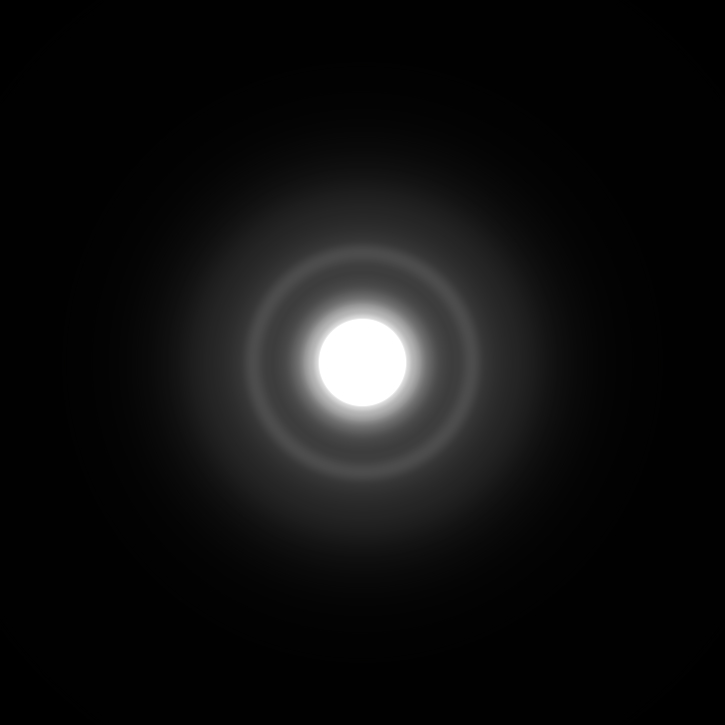
\includegraphics[height=\resLen]{waveoptics/slab/N100_300nm.jpg} &
        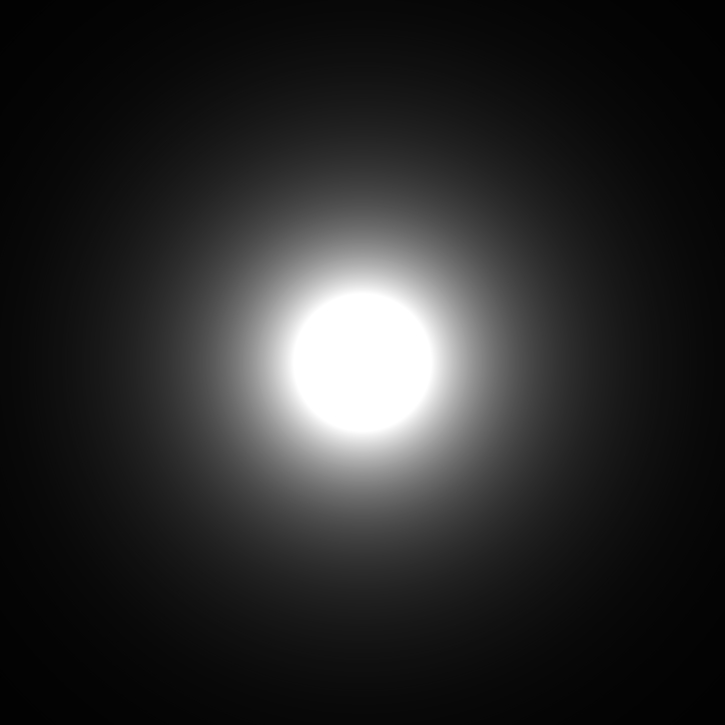
\includegraphics[height=\resLen]{waveoptics/slab/N100_500nm.jpg} &
        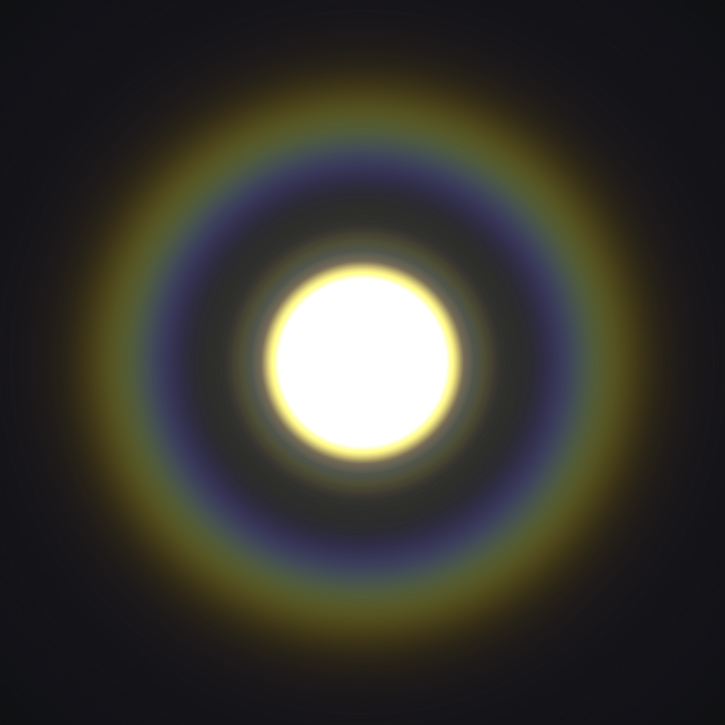
\includegraphics[height=\resLen]{waveoptics/slab/color.jpg} & 
        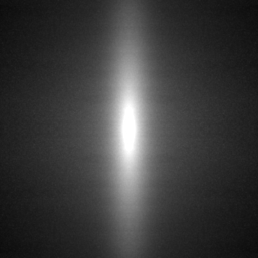
\includegraphics[height=\resLen]{waveoptics/slab/aniso_y.jpg} &
        
\includegraphics[height=\resLen]{waveoptics/slab/pos.jpg}
        \\
        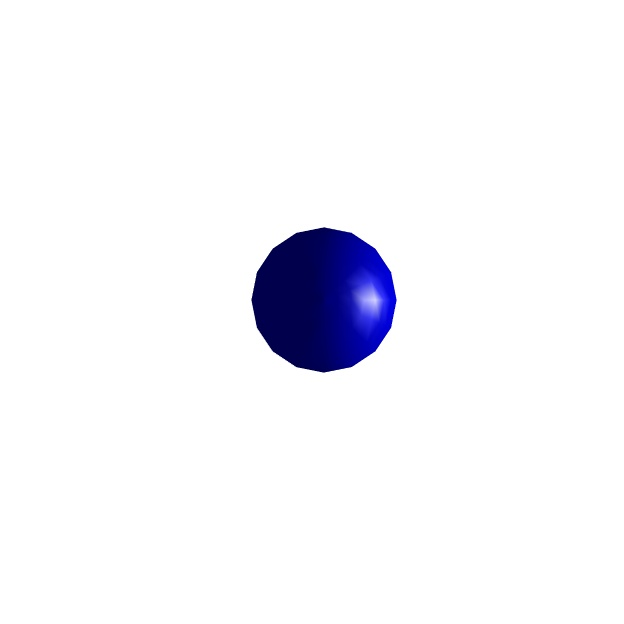
\includegraphics[height=\resLen]{waveoptics/particle/300nm_N1.jpg} &
        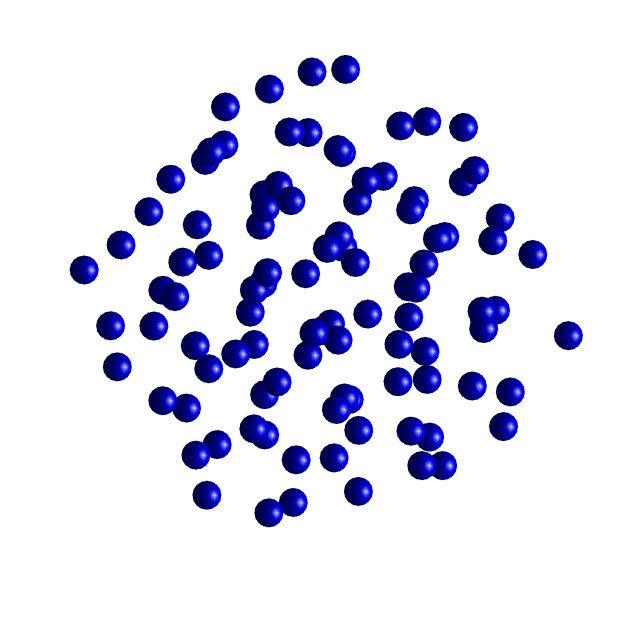
\includegraphics[height=\resLen]{waveoptics/particle/300nm_N100.jpg} &
        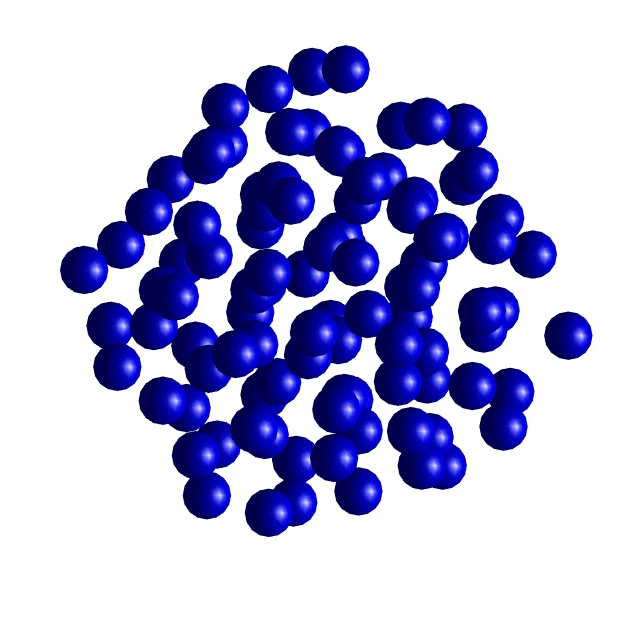
\includegraphics[height=\resLen]{waveoptics/particle/500nm_N100.jpg} &
        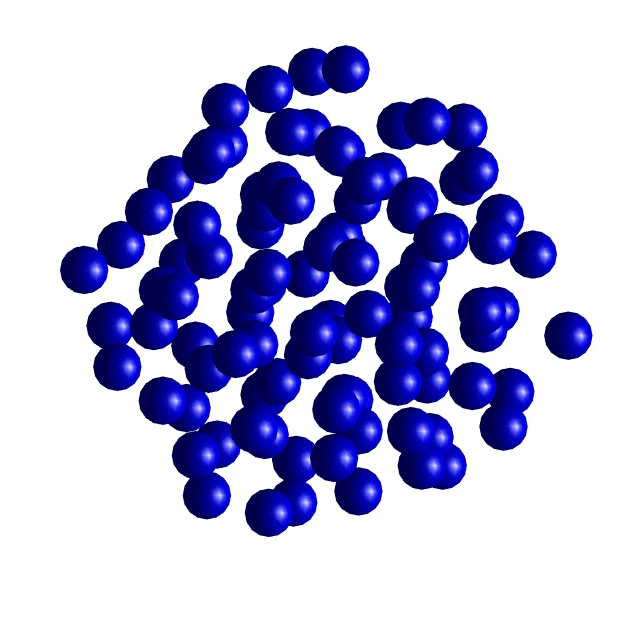
\includegraphics[height=\resLen]{waveoptics/particle/500nm_N100.jpg} &
        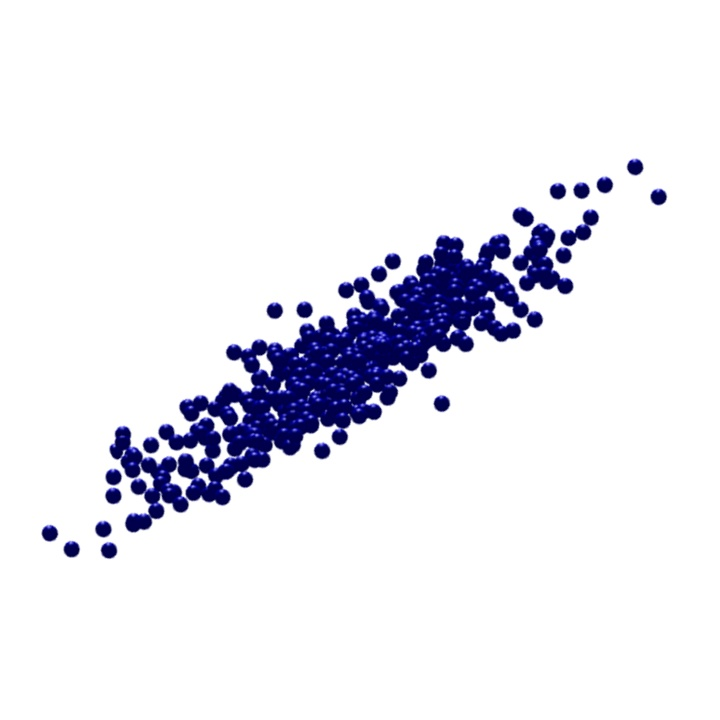
\includegraphics[height=\resLen]{waveoptics/particle/aniso.jpg} &
        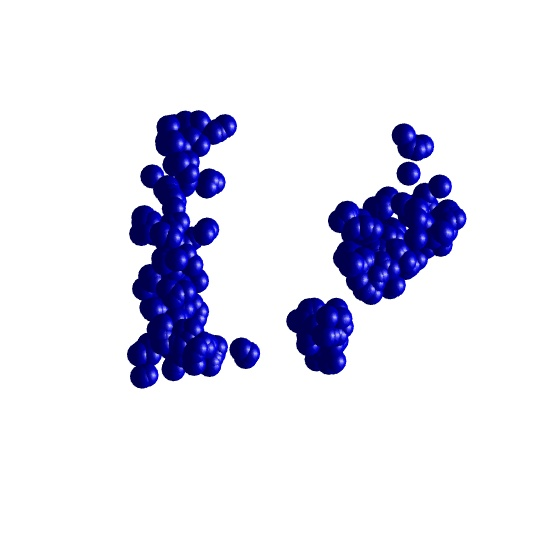
\includegraphics[height=\resLen]{waveoptics/particle/pos.jpg}
        \\
        $\Ncls=1$   &
        $\Ncls=100$ &
        $\Ncls=100$ &
        $\Ncls=100$ & 
        $\Ncls=100$ &
        $\Ncls=100$
        \\
        $a_i=300\text{nm}$ &
		$a_i=300\text{nm}$ &
		$a_i=500\text{nm}$ &
		$a_i=500\text{nm}$ & 
		$a_i=500\text{nm}$ &
		$a_i=500\text{nm}$
		\\
        Isotropic & Isotropic & Isotropic & Isotropic & Anisotropic & Pos. correlated
        \\
        $\lambda=700\text{nm}$ &
        $\lambda=700\text{nm}$ &
        $\lambda=700\text{nm}$ &
        Multi-spectral &
        $\lambda=700\text{nm}$ &
        $\lambda=400\text{nm}$
    \end{tabular}
    \caption[Teaser]{\label{fig:waveoptics:teaser}
        We introduce a new technique to compute bulk scattering parameters (i.e., the extinction and scattering coefficients as well as the single-scattering phase function) in a systematic fashion. By considering wave optical effects and particle (scatterer) interactions at the microscopic level, our technique enjoys the generality of supporting a wide range of media (e.g., isotropic, anisotropic, and correlated).
        In this figure, we show renderings of thin slabs lit with a small area light from behind (top).
        Additionally, we show visualizations of the corresponding particle distributions (middle) as well as per-cluster particle counts~$\Ncls$ radii $a_i$ (bottom).
    }
\end{figure}

\section{Introduction}
\label{sec:waveoptics:intro}

Participating media and translucent materials---such as marble, milk, wax, and human skin---are ubiquitous in the real world. These materials allow light to penetrate their surfaces and scatter in the interior. 

In computational optics and computer graphics, how light interacts with participating media and translucent materials is typically modeled using the radiative transfer theory (RTT). Under this formulation, a participating medium consists of microscopic particles (\emph{scatterers}) randomly dispersed in some homogeneous embedding medium. After entering a translucent material, light travels in straight lines in the embedding medium and occasionally collides with a particle and gets redirected into a new direction. To capture the macroscopic behavior of light, the RTT uses a statistical description of the particles (the medium bulk parameters), namely the extinction coefficient $\sigT$ (aka. optical density), the scattering coefficient $\sigS$, and the phase function $\phase$.

While purely phenomenological in origin, the RTT has been demonstrated a corollary of Maxwell equations, under the assumption of far-field or independent scattering \cite{mishchenko2002vector}. Therefore, these optical bulk parameters can be obtained from first principles, using e.g. Lorenz-Mie theory \cite{hulst1981light,frisvad2007computing}. However, although very successful in practice, this theory neglects the interactions occurring between particles in their near-field, including wave-optics effects such as diffraction and interference with neighbor particles. Consequently, Lorenz-Mie theory is largely limited to isotropic media with relatively low packing rates.


Previously, the classical radiative transfer theory has been generalized to handle materials with (statistically) organized microstructures. 
Anisotropic media \cite{jakob2010radiative}, for instance, have bulk scattering parameters with stronger directional dependency compared to isotropic media.
Additionally, media comprised of particles with correlated locations can exhibit non-exponential transmittance and characteristic scattering profiles \cite{bitterli2018radiative,jarabo2018radiative}.
Although several empirical models have been proposed to model these media, these still base on the very same far-field assumption of Lorenz-Mie scattering. Therefore, techniques capable of computing the bulk optical parameters of a material, based its microscopic properties, have been lacking.

In this chapter, we bridge this gap by introducing a new technique to systematically and rigorously compute the bulk scattering parameters.
The elementary building block of our technique is \emph{particle clusters} in which individual particles follow user-specified distributions.
Within a cluster, we consider full near-field light transport effects; Between clusters, on the contrary, we use a far-field approximation to allow efficient modeling of macroscopic level light transport.

Our formulation is derived from first principles of light transport (i.e., Maxwell electromagnetism) and reduces to the Lorenz-Mie theory in the special case of single-particle scatterers. Based on this formulation, we demonstrate how the bulk parameters can be computed numerically. Using our technique, we systematically generate radiative transfer optical parameters capturing multi-spectral, anisotropic, and correlated scattering effects for particles with arbitrary distributions (Figure \ref{fig:waveoptics:teaser}).

Concretely, our contributions include:
\begin{itemize}
    \item Establishing a computational framework for modeling light scattering from clusters of particles (\S\ref{sec:waveoptics:ours_theory}).
    %
    \item Showing how radiatve transfer parameters can be computed numerically based on our formulation (\S\ref{sec:waveoptics:ours_numerical}).
    %
    \item Demonstrating how our technique can be applied to systematically compute scattering parameters for a variety of participating media (\S\ref{sec:waveoptics:results}).
\end{itemize}

\section{Related Work}
\label{sec:waveoptics:related}

\paragraph{Radiative Transfer. } 
Simulating the propagation of light in participating media has been widely studied in graphics \cite{novak2018monte}, building upon the radiative transfer equation (RTE), introduced 125 years ago by von Lommel \cite{lommel1889photometrie} (see \cite{mishchenko2013125} for a historical perspective). 

This escalar radiative formulation has been extended in graphics accounting for anisotropic \cite{jakob2010radiative}, refractive \cite{ament2014refractive}, bispectral \cite{gutierrez2008visualizing}, or spatially-correlated media \cite{jarabo2018radiative,bitterli2018radiative}. All these works assume a radiometric light transport model, establishing no connections with the electromagnetic behaviour governing light transport. 

From a wave optics perspective, a few works have generalized light transport in media to account for wave-based properties, including polarized light transport \cite{wilkie2001combined,Jarabo2018bidirectional}, or coherence \cite{bar2019monte}. This last work is of special relevance, given that it was able to simulate purely wave-based phenomena such as speckle or coherent back-scattering on top of a radiative model. 

All these works build on the assumption of the far-field approximation and independent scattering, which largely simplifies computations. A notable exception is the near-field model proposed by Bar et al.\cite{bar2020rendering}, that renders speckle statistics in the near-field zone of the camera, although it still considers independent far-field scattering between particles. In contrast, in this work we explicitly relate the radiometric light transport modeled by the RTE with physics-based optics based on electromagnetism, and generalize the independent scattering approximation to account clusters of particles in the near field. 


\paragraph{Modeling scattering in media}

The phase function models the average scattering distribution at an interaction with the medium. A common approach is to use simple phenomenological models, such as the Henyey-Greenstein phase function \cite{henyey1941diffuse} or mixtures of von Mishes-Fisher distributions \cite{gkioulekas2013understanding}, as well as other functions modeling the scattering of idealized anistropic particles \cite{zhao2011building,heitz2015sggx}; however, these methods lack an explicit relationship with the underlying microscopic material properties. Under the assumption of geometric optics, several works have proposed to precompute the phase functions of more complex particles for granular materials \cite{meng2015multi,muller2016efficient} or cloth fibers \cite{aliaga2017appearance} using explicit path tracing, by neglecting wave effects. 

A more rigorous phase function is based on the Lorenz-Mie theory \cite{hulst1981light}, which provides closed-form solutions for the Maxwell's equations for spherical particles \cite{jackel1997modeling,frisvad2007computing}. Sadeghi et al. \cite{sadeghi2012physically} generalized the Lorenz-Mie theory to larger non-spherical particles in the context of accurately modeling rainbows. To avoid the expensive sum series of the Lorenz-Mie theory, Guo et al. \cite{guo2021rendering} proposed to use the geometric optics approximation \cite{glantschnig1981light}, which give a good approximation to Lorenz-Mie theory for larger particles at significantly lower cost. 

All these approaches provide accurate rigorous solutions to the far-field scattering of disperse particles. 

Beyond Lorenz-Mie, several exact rigorous solutions have been proposed for computing  electromagnetic scattering of particles in media, including the finite elements method (FEM), the finite difference time domain (FDTD) method, or the boundary elements method (BEM) \cite{wu1977scattering}, which solve the Maxwell's equations for arbitrary shapes. Xia et al. \cite{xia2020wave} proposed using BEM for accurately precomputing the far-field scattering of individual fibers. Unfortunately these methods are very slow as the number of particles increase, limiting its applicability to individual elements in problems with reduced dimensionality. 

The T-matrix method \cite{waterman1965matrix} generalizes the Lorentz-Mie theory to particles of arbitrary shape in both the near- and far-fields, with the only assumption of the computed field being outside a sphere surrounding the particles. This method was later extended to clusters of multiple particles \cite{peterson1973t,mackowski2011multiple}. We leverage the T-matrix method for computing the scattering of groups of particles. 

\paragraph{Wave optics in surface scattering} 
Inspired on the vast background on electromagnetic surface scattering in optics (see \cite{frisvad2020survey} for a general survey), several works in graphics have taken into account relevant wave effects including diffraction-aware BSDFs \cite{he1991comprehensive,stam1999diffraction,cuypers2012reflectance,dong2015predicting,holzschuch2017two, toisoul2017practical, werner2017scratch,yan2018rendering},  goniochromatic patterns due to thin-layer interference \cite{smits1992newton,gondek1994wavelength,belcour2017practical,guillen2020general} or birefringence \cite{steinberg2019analytic}. These works assume single scattering, with no interaction between different particles with a few exceptions that assume full incoherence after single scattering \cite{falster2020computing,guillen2020general}. Notably, Moravec \cite{moravec19813d} and Musbach et al. \cite{musbach2013full} computed the full electromagnetic surface scattering by solving the full wave propagation using the FDTD. 


\section{Preliminaries}
\label{sec:waveoptics:prelim}

We now briefly revisit the basics on first principles of (classical) light transport theory based on Maxwell electromagnetism. Table \ref{tab:waveoptics:notation} summarize the symbols using along the paper.

\input{tex/waveoptics/tab/notation}

\subsection{Electromagnetic Scattering}
\label{ssec:prelim_maxwells}

The propagation of a time-harmonic monochromatic electromagnetic field with frequency $\sFreq$ is defined by the Maxwell curl equations as
\begin{equation}
    \begin{aligned}
        \Curl\EField(\px) &= \img\,\sFreq\,\sPermeability(\px)\,\MField(\px),\\
        \Curl\MField(\px) &= \img\,\sFreq\,\sPermittivity(\px)\,\EField(\px),
    \end{aligned}
    \label{eq:maxwell}
\end{equation}
where $\Curl\cdot$ is the curl operator; $\EField(\px)$ and $\MField(\px)$ indicate, respectively, the (vector-valued) electric and magnetic fields at $\px$; $\sPermeability(\px)$ and $\sPermittivity(\px)$ denote the (scalar-valued) magnetic permeability and electric permittivity at $\px$, respectively; and $\img := \sqrt{-1}$ is the imaginary unit.

Assuming a non-magnetic medium satisfying $\sPermeability(\px) = \sPermeability_0$ with $\sPermeability_0$ being the magnetic permeability of a vacuum, \Eq{eq:maxwell} reduces to the electric field wave equation
\begin{equation}
    \nabla^2\times\EField(\px) - k^2\,\EField(\px) = 0,
    \label{eq:efieldwave}
\end{equation}
where $k(\px) = \sFreq\sqrt{\sPermittivity(\px)\sPermeability_0}$ is the medium's wave number at $\px$. 

We now assume an infinite homogeneous isotropic medium with permittivity $\sPermittivity_1$, filled with scatterers bounded by a finite disjoint region $V$, with potentially inhomogeneous permittivity $\sPermittivity_2(\px)$. Under this assumption, we can solve \Eq{eq:efieldwave} by expressing it as the \emph{volume integral equation} (see \S 3.1 of Mishchenko's work \cite{mishchenko2006multiple} for a step-by-step derivation) as the sum of the incident field $\IncEField(\px)$ and the scattered field $\ScaEField(\px)$ due to inhomogeneities in the medium in the form of scatterers:
\begin{align}
    \EField(\px) & = \IncEField(\px) + \ScaEField(\px) \\
    & =\IncEField(\px) + k_1^2\,\int_V [\sIOR^2(\px')-1] \,\sGreen(\px,\px') \,\EField(\px') \diff{\px'},
    \label{eq:vri}
\end{align}
with $k_1$ the wave number at the hosting medium, $\sIOR(\px) = k_2(\px)/k_1$ the index of refraction of the interior regions $V$ with respect to the hosting medium, and $\sGreen(\px,\px')$ the free-space dyadic Green's function defined as:
\begin{equation}
    \sGreen(\px,\px') = \left(\sIdDyad + k_1^{-2}\,\nabla\otimes\nabla\right) \frac{\exp(\img\,k_1 \,|\px-\px'|)}{4\pi\,|\px-\px'|},
    \label{eq:greenfunc}
\end{equation}
where $\sIdDyad$ is the identity dyad, and $. \otimes .$ denotes the dyadic product of two vectors. Intuitively, \Eq{eq:vri} models the scattering field as the superposition of the spherical wavelets resulting from a change of permitivitty (i.e. with $\sIOR(\px')\neq1$). Note also the recursive nature of \Eq{eq:vri}; we will deal with this recursivity in the following section, computing $\ScaEField(\px)$ as a function of the incident field $\IncEField(\px)$. 

\subsection{Foldy-Lax Equations}
\label{ssec:foldy-lax}

We now consider a medium filled with $N$ finite discrete particles with volume $V_i$ and index of refraction $\sIOR_i(\px)$. Considering an incident E-field $\IncEField(\px)$, we can rewrite \Eq{eq:vri} as
\begin{equation}
    \EField(\px) = \IncEField(\px) + \int_{\Real^3} U(\px')\,\sGreen(\px,\px') \cdot \EField(\px') \diff{\px'},
    \label{eq:EfieldParticles}
\end{equation}
where $\sGreen(\px,\px')$ is the dyadic Green's function~\eqref{eq:greenfunc}, and $U(\px)$ the potential function given by
\begin{equation}
    U(\px) = \sum_{i=1}^{N} U_i(\px) \quad \text{with} \quad U_i(\px) = \begin{cases} 
    0, & (\px \notin V_i)\\ 
    k_1^2[\sIOR_i^2(\px)-1]. & (\px \in V_i)
    \end{cases}
    \label{eq:potential}
\end{equation}
By combining \Eqs{eq:EfieldParticles}{eq:potential}, we can express the field at any position $\px\in\Real^3$ following the so-called \emph{Foldy-Lax equation} \cite{foldy1945multiple,lax1951multiple} as
\begin{equation}
\EField(\px) = \IncEField(\px) + \sum_{i=1}^N \overbrace{\int_{V_i} \sGreen(\px,\px')\cdot \int_{V_i} \dyad{T}_i(\px',\px'') \cdot  \EField_i(\px'') \diff{\px''}\,\diff{\px'}}^{\eqdef \,\ScaEField_i(\px)}    \label{eq:foldylax}
\end{equation}
with $\ScaEField_i(\px)$ and $\EField_i(\px)$ the scattered and partial field of particle $i$, and $\dyad{T}_j(\px,\px')$ $\dyad{T}_i(\px,\px')$ the dyad transition operator for particle $i$ defined as \cite{tsang1985theory} 
\begin{equation}
\label{eq:dyadtransition}
    \begin{split}
        \dyad{T}_i(\px,\px') =\;& U_i(\px) \,\delta(\px-\px')\,\sIdDyad + U_i(\px) \int_{V_i} \sGreen(\px,\px'') \cdot \dyad{T}(\px'',\px') \diff{\px''},
    \end{split}
\end{equation}
with $\delta(x)$ the Dirac delta. 
The partial field at particle $i$ is defined as $\EField_i(\px)=\IncEField(\px) + \sum_{j(\neq i)=1}^N \ExcEField_{ij}(\px)$, where the partial exciting field $\ExcEField_{ij}(\px)$ from particles $j$ to $i$ is 
\begin{equation}
\ExcEField_{ij}(\px) = \int_{V_j} \sGreen(\px,\px')\int_{V_j} \dyad{T}_j(\px',\px'') \EField_j(\px'') \diff{\px''}\,\diff{\px'},
\label{eq:excfield}
\end{equation}
with $\px\in V_i$. Note that the scattered and exciting fields for particle $j$ have essentially the same form. 
As shown by Mishchenko \cite{mishchenko2002vector}, the Foldy-Lax equation~\eqref{eq:foldylax} solves exactly the volume integral equation~\eqref{eq:vri} for multiple arbitrary particles in the medium, without any assumptions on their composition or packing rate, beyond the assumption of a homogeneous hosting medium.

\input{tex/waveoptics/fig/diagram}

\paragraph{Far-field Foldy-Lax Equations}
\Eq{eq:excfield} defines the exact exciting field resulting from the scattering by particle~$j$ on particle~$i$.
However, if the distance $\tPx_{ij} \defeq \| \Px_i - \Px_j \|$ between particles (with $\Px_i$ denoting the center of particle $i$) is large, we can approximate the propagation distance between any point $\px \in V_i$ and $\px' \in V_j$ as
\begin{equation}
    \| \px - \px' \| \approx \tPx_{ij} + (\dPx_{ij} \cdot {\Delta}\px) -  (\dPx_{ij} \cdot {\Delta}\px'),
\end{equation}
with $\dPx_{ij} \defeq (\Px_i - \Px_j)/\tPx_{ij}$, ${\Delta}\px \defeq \px - \Px_i$ and ${\Delta}\px' \defeq \px' - \Px_j$ (see Figure \ref{fig:waveoptics:diagram}, left).
With this approximation, we can now express $\ExcEField_{ij}(\px)$ for a point $\px \in V_i$ using its \emph{far-field} approximation, as:%
\footnote{We note that, accordingly to Mishchenko \cite{mishchenko2006multiple}, the product would require to multiply the integrand by the dyad $(\sIdDyad - \dPx_{ij}\otimes\dPx_{ij})$ to ensure a transverse planar field; we remove it for clarity.}
\begin{equation}
    \begin{split}
        & \ExcEField_{ij}(\px)\\
        \approx\;& \frac{\E^{\img k_1 (\tPx_{ij}+\dPx_{ij}\cdot{\Delta}\px)}}{4\pi\tPx_{ij}} \int_{V_j} \sGreenProp(\dPx_{ij},{\Delta}\px') \int_{V_j} \dyad{T}_j(\px',\px'')\cdot \EField_j(\px'') \diff{\px''}\,\diff{\px'} \\
        =\;& \frac{\exp(\img k_1 \,\tPx_{ij})}{\tPx_{ij}} 
        \sGreenProp(\dPx_{ij}, \Delta \px) \,\ExcEField_{1ij}(\dPx_{ij}),
    \end{split}
    \label{eq:excfieldfar}
    \raisetag{17pt}
\end{equation}
where: $\px \in V_i$ is a point in particle $i$; $\sGreenProp(\dw, \Delta \px)=\exp(\img k_1 \,\dPx_{ij}\cdot{\Delta}\px)$; and $\ExcEField_{1ij}$ is the far-field exciting field from particle $j$ to particle $i$ that is solely characterized by the propagation direction $\dPx_{ij}$. In order for \Eq{eq:excfieldfar} to be valid, the distance $\tPx_{ij}$ needs to hold the far-field criteria, which relates the $\tPx_{ij}$ with the radius of the particle $\radius_j$ following the inequality~\cite{mishchenko2006multiple}:
\begin{equation}
    k_1 \tPx_{ij} \gg \max\left(1, \frac{k_1^2\radius_j^2}{2}\right).
    \label{eq:farfield}
\end{equation}
This far-field assumption is both the basis for the Lorenz-Mie theory \cite{hulst1981light} (to model electromagnetic scattering from small spherical particles) and, as shown by Mishchenko \cite{mishchenko2002vector}, at the core of the radiative transfer theory.

In the following, we relax the assumption of near field scattering and compute the Foldy-Lax equations for clusters of particles for both the near- and far-field regions. Then, we use them to compute the scattering matrix to be used in the RTE to efficiently approximate light transport between clusters of particles. 

\section{Scattering from Clusters of Particles}
\label{sec:waveoptics:ours_theory}

In this section, we present our main theoretical result: the far-field approximated scattering dyad relating a field incoming at a particle, which will be shown in \Eq{eq:farscatdyad}.
This dyad can then be used to compute a medium's bulk scattering parameters, which we will discuss in \S\ref{ssec:ours_RTT}.

The two forms of computing the exciting field from particle $j$ to $i$ [\Eqs{eq:excfield}{eq:excfieldfar}] suggest that we can consider two subsets of particles $j$ depending on their distance with respect to the point of interest $\bfr$: One set of $\Nnear$ particles in the near field and another set of $\Nfar$ particles in the far field. With that, we can now calculate the exciting field in particle $i$ as:
\begin{equation}
    \bfE_i(\bfr)= \bfEi(\bfr) + \sum_{j(\neq i)=1}^\Nnear \bfEe_{ij}(\bfr) + \sum_{k=1}^{\Nfar} \bfEe_{ik}(\bfr).
    \label{eq:foldylaxtwo}
\end{equation}

In what follows, we derive the far-field Foldy-Lax equations for groups of particles where a cluster of these particles are in their respective near-field region, while the other elements in the system are in the far field. For the simplicity of our derivations, we consider a single far-field incident field in the cluster, and assume that the far-field particles $k$ do not have neighbor particles in their respective near field region.

More formally, we now consider a cluster $\Cls$ of $N_\Cls$ particles, where all particles $i\in\Cls$ are in their respective near-field region, and that the particles of the cluster have a bounding sphere centered at $\bfR_\Cls$ with radius $a_\Cls$ (see Figure \ref{fig:waveoptics:diagram}, middle). 

Since both the incident field $\bfEi(\bfr)$ and the exciting field $\bfEe_{\Cls k}(\bfr)$ from particle $k$ are in the far-field region, we can assume both fields to be planar waves defined as
\begin{align}
    \label{eq:farincfieldcluster}
    \bfEi(\bfr) &= \bfEi_0 \,\exp(\Img k_1 \hatbfn \cdot \Delta \bfr) = \bfEi_0\,g(\hatbfn, \Delta \bfr) , \\
    \bfEe_{\Cls k}(\bfr) &= \bfEe_{0\Cls k}\,\exp(\Img k_1 \hatbfR_{\Cls k} \cdot \Delta \bfr) =  \bfEe_{0\Cls k}\,g(\hatbfR_{\Cls k}, \Delta \bfr), 
    \label{eq:farexcfieldcluster} 
\end{align}
with $\bfEi_0$ the amplitude of the planar incident field, $\hatbfn$ its direction, and $\Delta \bfr=\bfr-\bfR_\Cls$. Equivalently, $\bfEe_{0\Cls k}=\frac{\exp(\Img k_1 \,R_{\Cls k})}{R_{\Cls k}}\,\bfEe_{1\Cls k}(\hatbfR_{\Cls k})$  is the amplitude of the exciting field at $\Cls$ from particle $k$, and $\hatbfR_{\Cls k}$ its direction. 

Now, let us slightly abuse the dot product notation, remove the dependency on the spatial dependency on each term, and use $(\varphi_1 \cdot \varphi_2) = \int \varphi_1(x)\,\varphi_2(x) \intd x$ for scalar-valued functions $\varphi_1$ and $\varphi_2$. From the far-field assumptions, plugging \Eq{eq:foldylaxtwo} into the definition of the scattered field from particle $i\in\Cls$ in Equation~\eqref{eq:foldylax} (with $\Nnear=\Ncls$) yields
\begin{equation}
    \label{eq:scafieldcluster1}
    \begin{split}
        \bfEs_i(\bfr) &= \dyad{G} \cdot \dyad{T}_i\cdot \bfE_i\\
        & = \dyad{G} \cdot \dyad{T}_i \cdot \left[\bfEi + \sum_{k=1}^{\Nfar} \bfEe_{\Cls k}+ \sum_{j(\neq i)=1}^{\Ncls} \bfEe_{ij} \right].
    \end{split}        
\end{equation}
By recursively expanding $\bfEe_{ij}$ and some algebraic operations (see the supplemental for the full derivation), this results into 
\begin{align}
    \label{eq:scafieldcluster5}
    \bfEs_i(\bfr) &= \bfE_0 \, \dyad{G} \cdot \dyad{T}_i \cdot \Bigg[ g(\hatbfn) + \sum_{j(\neq i)=1}^{\Ncls} \left[...\right]_j^{g(\hatbfn)} \Bigg] \\
    & + \sum_{k=1}^{\Nfar} \bfEe_{0\Cls j}\,\left[ \dyad{G} \cdot \dyad{T}_i \cdot \Bigg[ g(\hatbfR_{\Cls k}) + \sum_{j(\neq i)=1}^{\Ncls} \left[...\right]_j^{g(\hatbfR_{\Cls k})}\Bigg]\right]. \nonumber 
\end{align}
where the "$[...]_l^\varphi$" term represents the recursivity as
\begin{equation}
    [...]_j^\varphi= \dyad{G} \cdot \dyad{T}_j \cdot \left[\varphi + \sum_{l(\neq j)=1}^{\Ncls} \left[...\right]_l^\varphi\right] \,.
\end{equation}
Note that each element in the sum in \Eq{eq:scafieldcluster5} above is the result of the amplitude of the far-field incident or exciting fields, and a series that encode all the near-field scattering in the cluster $\Cls$. We can thus define the scattering dyad $\dyad{A}_i^\text{near}(\hatbfni,\bfr)$ relating a unit-amplitude planar incident field at particle $i$ from direction $\hatbfni$ with the scattered field at point $\bfr$ as
\begin{equation}
    \dyad{A}_i^\text{near}(\hatbfni,\bfr) = \dyad{G} \cdot \dyad{T}_i\cdot \Bigg[ g(\hatbfni) + \sum_{j(\neq i)=1}^{\Ncls} \left[...\right]_j^{g(\hatbfni)} \Bigg].
    \label{eq:scatdyad_near}
\end{equation}
By considering constant $\bfEi_0$ and $\bfEe_{0\Cls k}$ for the whole cluster $\Cls$, we can compute the cluster's scattering dyad as:
\begin{equation}
    \dyad{A}_\Cls^\text{near}(\hatbfni,\bfr) = \sum_{i=1}^{N_\Cls} \dyad{A}_i(\hatbfni,\bfr),
    \label{eq:scatdyadcluster_near}
\end{equation}
which defines the scattered field for a unit-amplitude incoming planar field in a scene consisting of the particles forming cluster $\Cls$.
In practice, the scattering dyad $\dyad{A}_\Cls^\text{near}(\hatbfni,\bfr)$ can be computed numerically using standard methods from computational electromagnetics \cite{mishchenko2014electromagnetic}.


\paragraph{Far-field approximation}
\Eq{eq:scatdyad_near} represents the general form of the scattering dyad for particle $i$, which results into a five-dimensional function. Assuming that $\bfr$ is in the far-field region of a particle $i\in\Cls$, by using the far-field approximation of the scattered or exciting field~\eqref{eq:excfieldfar} (we refer to the supplemental document for the derivation), we get the scattered field by particle $i$ as
\begin{align}
    \bfEs_i(\bfr) \approx \frac{\Exp^{\Img k_1 R_i}}{R_i} \Big(\bfE_0 \,  \dyad{A}_i(\hatbfn,\hatbfR_i) 
    + \sum_{k=1}^{\Nfar} \bfEe_{0\Cls k} \, \dyad{A}_i(\hatbfR_{\Cls k},\hatbfR_i) \Big),
    \label{eq:farscatfield}
\end{align}
with $R_i=|\bfr-\bfR_i|$ and $\hatbfR_i=\frac{\bfr-\bfR_i}{R_i}$, and
\begin{equation}
    \label{eq:farscatdyad}
    \boxed{%
        \dyad{A}_i(\hatbfnis) = \frac{g(\hatbfns)\cdot \dyad{T}_i}{4\pi} \cdot\Bigg[ g(\hatbfni) + \sum_{j(\neq i)=1}^{\Ncls} \left[...\right]_j^{g(\hatbfni)} \Bigg].
    }
\end{equation}
Finally, since $\hatbfR_i\approx\hatbfR_\Cls$ for all particles $i\in\Cls$, we can approximate the far-field scattered field of cluster $\Cls$ as
\begin{equation}
    \bfEs_\Cls(\bfr) = \frac{\Exp^{\Img k_1 R_\Cls}}{R_\Cls}\Big( \bfE_0 \,  \dyad{A}_\Cls(\hatbfn,\hatbfR_\Cls) + \sum_{k=1}^{\Nfar} \bfEe_{0\Cls k} \, \dyad{A}_\Cls(\hatbfR_{\Cls k},\hatbfR_\Cls) \Big),
    \label{eq:farscatfieldcluster}
\end{equation}
where
\begin{equation}
   \dyad{A}_\Cls(\hatbfnis) = \sum_{i=1}^{N_\Cls}\dyad{A}_i(\hatbfnis),
   \label{eq:farscatdyadC}
\end{equation}
is the far-field scattering dyad of cluster $\Cls$.

Thus, by grouping the individual particles into $\Ncls$ near-field clusters, and assuming that all clusters and observation point $\bfr$ lay in their respective far field, we can approximate the Foldy-Lax equation~\eqref{eq:foldylax} as
\begin{equation}
    \bfE(\bfr) = \bfEi(\bfr) + \sum_{\Cls_j=1}^{\Ncls} \bfEs_{\Cls_j}(\bfr),
    \label{eq:foldylaxcluster}
\end{equation}
with $\bfEs_{\Cls_j}(\bfr)$ the scattered field at cluster $\Cls_j$. 


\subsection{Relationship with the Radiative Transfer Theory}
\label{ssec:ours_RTT}

The scattering dyad $\dyad{A}_\Cls(\hatbfnis)$ given by \Eq{eq:farscatdyadC} models how a particle cluster $\Cls$ scatters a planar unit-amplitude incident field in the far field region. However, for rendering we are generally interested on the average field intensity (i.e. radiance). 

As shown by Mishchenko \cite{mishchenko2002vector}, the radiative transfer equation (RTE) directly derives from the far-field Foldy-Lax equations under three additional assumptions: (i)~The amount of coherent backscattering is negligible; (ii)~The particles are randomly distributed according to some distribution $p(R_i,\xi_i)$, with $R_i$ and $\xi$ denoting, respectively, the position and properties of a particle $i$; and (iii) We are interested on the average field $\EV{\bfE(\bfr)}$. 

Following these assumptions, and after a lengthy derivation, Mishchenko demonstrates that the bulk scattering properties can be obtained from the far-field Foldy-Lax form, and in particular from the scattering dyad $\dyad{A}(\hatbfnis)$. Let us first assume that the distribution of particle properties $\xi$ are independent of the particles position, and compute the average scattering dyad $\EV{\dyad{A}(\hatbfnis)} = \int_\Omega \dyad{A}_i(\hatbfnis) p(\xi_i) \intd \xi_i$. 

Then, note that the Foldy-Lax equation for clusters of particles~\eqref{eq:foldylaxcluster}, we derived above has the same form as the original Foldy-Lax equation~\eqref{eq:foldylax}. Thus, by the same derivation followed by Mishchenko we get to an equivalent RTE based on the scattering dyad of clusters. 

\paragraph{Computing the scattering parameters}
By taking the vectors of the parallel and perpendicular polarization $\hatbmthetai$ and $\hatbmphii$ of the incident field as shown in Figure \ref{fig:waveoptics:diagram} (right), and equivalently for the scattered field $\hatbmthetas$ and $\hatbmphis$, we can compute the polarized scattering components $\bmStheta$ and $\bmSphi$ from the cluster's scattering dyad $\dyad{A}_\Cls(\hatbfnis)$ as
\begin{align}
  \bmStheta(\hatbfnis) &= \hatbmthetas \cdot \EV{\dyad{A}_\Cls(\hatbfnis)} \cdot \hatbmthetai, \nonumber \\
  \bmSphi(\hatbfnis) &= \hatbmphis \cdot \EV{\dyad{A}_\Cls(\hatbfnis)} \cdot \hatbmphii.
\end{align}
Then, based on the two scattering components $\bmStheta$ and $\bmSphi$, we can obtain the optical parameters of the medium as
\begin{align}
    \label{eq:crosstcluster}
    \Ct(\hatbfni) &= 4\pi \Re\left[\frac{\bmS(\hatbfni,\hatbfni)}{k_i^2}\right], \\
    \label{eq:crossscluster}
    \Cs(\hatbfni) &=\int_\bbSS \frac{|\bmStheta(\hatbfnis)|^2+|\bmSphi(\hatbfnis)|^2}{2k_1^2} \intd \hatbfns, \\
    \label{eq:phasecluster}
    \fp(\hatbfnis) &= \frac{|\bmStheta(\hatbfnis)|^2+|\bmSphi(\hatbfnis)|^2}{2k_1^2\Cs},
\end{align}
with $\bmS(\hatbfni,\hatbfni)=\bmSphi(\hatbfni,\hatbfni)=\bmStheta(\hatbfni,\hatbfni)$, and $\Re[x]$ returning the real part of a complex number $x$. Lastly, assuming a uniform distribution of clusters, we can compute the extinction and scattering coefficients as
\begin{align}
    \label{eq:sigmatcluster}
    \sigmat(\hatbfni) &= \Ct(\hatbfni) \frac{\rho}{\EV{\Ncls}}, \\
    \label{eq:sigmascluster}
    \sigmas(\hatbfni) &= \Cs(\hatbfni) \frac{\rho}{\EV{\Ncls}},
\end{align}
with $\rho$ the number of particles per differential volume, and $\EV{\Ncls}$ the average number of particles per cluster. Note that the optical properties defined in Equations~\eqref{eq:crosstcluster}--\eqref{eq:sigmascluster} are directionally dependent, so they are general and can represent both isotropic and anisotropic media. 


\subsection{Relationship with Independent Scattering}
\label{ssec:ours_indep_scat}

Most previous works rendering light transport in media \cite{novak2018monte} build on the assumption of independent scattering---that is, particles are in their respective far-field region.
It is easy to verify that this is a special case of \Eq{eq:foldylaxtwo} with $\Ncls=1$, causing 
the scattering dyad $\dyad{A}_\Cls$ of \Eq{eq:farscatdyadC} to reduce to
\begin{equation}
    \label{eq:farscatmie}
    \dyad{A}_\Cls(\hatbfnis) = \dyad{A}_i(\hatbfnis) = \frac{g(\hatbfns)\cdot \dyad{T}_i \cdot g(\hatbfni)}{4\pi},
\end{equation}
which encodes the scattered field in the far-field region of a particle when excited by an incident unit-amplitude planar field. 

The Lorenz-Mie theory \cite{hulst1981light} provides closed-form expressions for $\dyad{A}_i(\hatbfnis)$ for spheres and cylinders, while numerical solutions of $\dyad{A}_i(\hatbfnis)$ have been proposed for scatterers of arbitrary shapes via, for example, the T-matrix method \cite{waterman1965matrix}, or more recently based on the BEM for cylindrical fibers~\cite{xia2020wave}. Our work is therefore a generalization of these works to particles in the near field. 

\section{Computing the Bulk Scattering Parameters}
\label{sec:waveoptics:ours_numerical}

We now detail our numerical computations of the scattering dyad $\dyad{A}_\Cls(\hatbfnis)$ of \Eq{eq:farscatdyadC}, which in turn determines the bulk scattering parameters that can be directly used in any renderer supporting participating media. 

Computing $\dyad{A}_\Cls(\hatbfnis)$ essentially boils down to solving the time-harmonic Maxwell equations for an incident unit-amplitude planar field with direction $\hatbfni$. While several different methods exist for that purpose (see \S 16 of \cite{mishchenko2014electromagnetic} for an overview), we opt for the superposition T-matrix method \cite{mackowski1996calculation} that has been demonstrated efficient for moderately large $\Ncls$, can handle scatterers with arbitrary geometry, and is based on the principles of the Foldy-Lax equations, making it particularly appealing for our work. 

In practice, we use the open-source CUDA-based \texttt{CELES} solver \cite{egel2017celes}, which implements the T-matrix method proposed by Mackowski and Mishchenko \cite{mackowski2011multiple} for spherical or randomly rotated particles.
In our implementation, we focus on clusters of spherical particles.
Since the Lorenz-Mie theory also assumes spherical particles, this allows us to directly compare our results with those computed using the Lorenz-Mie theory. 

To compute the average scattering dyad $\EV{\dyad{A}_\Cls(\hatbfnis)}$, we average the scattered field of several random realizations of the clusters (each of which obtained by randomly sampling the position of the particles inside the cluster's bounding sphere).
As we will demonstrate in \S\ref{sec:waveoptics:results}, we use a wide array of distributions including particles uniformly distributed over the volume of the cluster, positively-correlated particles following Shaw et al. \cite{shaw2002super}, negatively-correlated particles using Poisson sampling of the sphere, and anisotropic distributions by uniformly sampling the particles on a oriented 2D disk.

Lastly, we represent the resulting phase function as well as the extinction and scattering cross sections as tabulated (i.e., piecewise constant) functions that can be used for rendering.

\section{Experiments}
\label{sec:waveoptics:results}

In this section, we first validate our technique by comparing bulk scattering parameters computed with our method and the Lorenz-Mie theory (\S\ref{ssec:result_validation}).
Then, we apply our technique described in \S\ref{sec:waveoptics:ours_theory} and \S\ref{sec:waveoptics:ours_numerical} to compute bulk scattering parameters for a wide range of participating media (\S\ref{ssec:result_main}).


\subsection{Validation}
\label{ssec:result_validation}

To validate our technique, we compare computed bulk scattering parameters provided by our implementation and \texttt{MiePlot} \cite{laven2011mieplot}, a free software based on the Lorenz-Mie theory.
We focus on the configuration where a cluster contains only one (spherical) particle as this is a fundamental assumption of the Lorenz-Mie theory.

\input{tex/waveoptics/fig/mie}

In Figure \ref{fig:waveoptics:mie}, we visualize computed single-scattering phase functions at the wavelength 600~nm with three particle radii (300, 600, and 900~nm).
We set the refractive index of the embedding medium to $(1.5 + 0.1\img)$.

Additionally, we show in Figure \ref{fig:waveoptics:mie2} the corresponding extinction and scattering cross sections $\cT$ and $\cS$ given by Equations~\eqref{eq:crosstcluster} and \eqref{eq:crossscluster}, respectively.
In all these examples, our computed scattering parameters match those predicted by the Lorenz-Mie theory perfectly.

\input{tex/waveoptics/fig/mie2}


\subsection{Main Results}
\label{ssec:result_main}
%
We now demonstrate the versatility of our technique by computing bulk scattering parameters for a range of participating media.
Please see Table~\ref{fig:waveoptics:time} for the performance statistics of our experiments.

\input{tex/waveoptics/tab/time}

\paragraph{Isotropic media}

In computer graphics, volumetric light transport effects are typically simulated using \emph{isotropic media} where the extinction and scattering coefficients $\sigT$, $\sigS$ are directionally independent, and the single-scattering phase function $\phase$ is formulated as a 1D function on the angle between the incident and scattered directions.

Our technique can produce bulk scattering parameters for isotropic media using particles distributed in radically symmetric densities.
We conduct a few ablation studies to demonstrate how different particle arrangements in a cluster affects the resulting parameters.
We use a wavelength of 600~nm for all these studies and represent the 1D phase functions as tabulated (i.e., piecewise constant) functions using 180 equal-sized bins.

\input{tex/waveoptics/fig/ablation}

\input{tex/waveoptics/fig/lucycompare}

In our first study, we use a cluster of 100 particles with radii 500~nm. Then, we vary the distances between particles (by using bounding spheres with different sizes and distributing particles uniformly in these spheres).
As shown in Figure \ref{fig:waveoptics:ablation} (a), the closer the particles are to each other, the more forward the resulting phase function is.
This is expected: With sparsely distributed particles, it is simpler for light to pass straightly through.

Our second ablation study examines the effect of particle size. With 100 uniformly distributed particles, we apply our technique to three particle sizes ($\radius_i$= 400, 500, and 600 nm).
As shown in Figure \ref{fig:waveoptics:ablation} (b), as we increase the particles radius, the phase function becomes more forward and increases its frequency. This agrees with the behaviour of single particles predicted by Lorenz-Mie theory. 

In our third study, we vary the number of particles in a cluster while keeping the particle size fixed to $\radius_i$=500 nm.
Figure \ref{fig:waveoptics:ablation} (c) shows that as we increase the number of particles, the phase function gets more forward and of higher-frequency, in a behaviour somewhat correlated with the particles size. This is the result of the increasing number of diffractive elements on the cluster, that instead of making scattering more diffuse (as predicted by geometric optics) increases its forward frequency. 

Lastly, we show in Figure \ref{fig:waveoptics:lucycompare} monochrome renderings using bulk scattering parameters obtained with varying combinations of particle count and radius.


\paragraph{Multi-spectral results}

Since our technique is derived using microphysical wave optics, it allows systematic generation of multi-spectral parameters based on a single (monochrome) configuration of particle cluster.

To demonstrate this, we use a configuration of 100 uniformly distributed particles (per cluster) with radius 500~nm and compute bulk scattering parameters at 50 wavelengths ranging from 400~nm to 700~nm.

\input{tex/waveoptics/fig/multiwave1}

\input{tex/waveoptics/fig/multiwave2}

In Figure \ref{fig:waveoptics:multiwave1}, we visualize the computed phase functions at three wavelengths as well as multi-spectral renderings of a backlit thin slab.
The smooth changes in scattering parameters across wavelength have resulted in a characteristic rainbow-like effect.
When using the single-particle configuration (with identical overall particle density per unit volume), the rainbow effect is missing.

Figure \ref{fig:waveoptics:multiwave2} shows renderings of the Lucy model using these scattering parameters.


\paragraph{Anisotropic media}

Anisotropic media allow the extinction and scattering coefficients $\sigT$, $\sigS$ to be directionally dependent, and have full 4D phase functions $\phase$.
Previously, although the scattering parameters of anisotropic media can be devised based on the microflake models \cite{jakob2010radiative,heitz2015sggx}, equivalences of the Lorenz-Mie theory, to our knowledge, have been lacking. 

\input{tex/waveoptics/fig/aniso1}

By using anisotropic particle distributions, our technique can generate bulk scattering parameters for anisotropic media.
To demonstrate this, we use a configuration where the cluster contains $\Ncls = 100$ particles following an anisotropic Gaussian distribution, as illustrated in Figure \ref{fig:waveoptics:aniso1}(a).
We tabulate the extinction and scattering cross sections using the latitude-longitude parameterization with a resolution of $180 \times 360$.
Due to the symmetry of the disc, the resulting phase function $\phase$ is three-dimensional, and we tabulated it with the resolution $90 \times 180 \times360$.

In Figure \ref{fig:waveoptics:aniso1}(b), we visualize slices of the computed single-scattering phase function $\phase$ with two incident directions $\dwi$.
In Figure \ref{fig:waveoptics:aniso2}, we show renderings of the Lucy model with three (spatially invariant) orientations.

\input{tex/waveoptics/fig/aniso2}


\paragraph{Correlated particles}

Finally, in Figure \ref{fig:waveoptics:correlated} we demonstrate the effect of particles correlation within the cluster, by analyzing particles distributed using both negative (Poisson sampled) and positive correlation \cite{jarabo2018radiative}. We compare the effect of introducing microscopic correlation on media where the clusters position is itself correlated, compared with uniformly distributed particles inside the clusters. These two levels of correlation have significant effect on the final appearance of the translucent materials. 

\input{tex/waveoptics/fig/correlated}

\section{Conclusion}
\label{sec:waveoptics:conclusion}

In this chapter, we introduce a new technique to systematically compute bulk scattering parameters for participating media. Built upon first principles of light transport (i.e., Maxwell electromagnetism), our technique models a translucent material as clusters of particles randomly distributed in embedding media. Our work generalizes the widely-used Lorenz-Mie theory for rigorously deriving optical properties of scattering media, and can be readily used in any radiative-based light transport simulator. 

We have demonstrated the significant effects of departing from the underlying assumptions of Lorenz-Mie theory, and the versatility for modeling a wide range of participating media by modifying the arrangement of particles within each cluster, including isotropic, anisotropic, and correlated media.


\chapter{Inverse Rendering for Macroscale Material Parameters}
\label{cpt:svbrdf}

\begin{figure}[h]
	\centering
	\setlength{\resLen}{6.25in}
	\setlength{\raiseLen}{0.35in}
	\addtolength{\tabcolsep}{-4pt}
	\begin{tabular}{cc}
		\raisebox{0.5\raiseLen}{\rotatebox[origin=c]{90}{\small Input}} &
		
\includegraphics[width=\resLen]{svbrdf/teaser/refs.jpg}
		\\[-2pt]
		\raisebox{\raiseLen}{\rotatebox[origin=c]{90}{\small Rendering}} &
		\animategraphics[width=\resLen,loop,alttext=]{5}{svbrdf/teaser/teaser_}{001}{024}
		\\[-2pt]
		\raisebox{\raiseLen}{\rotatebox[origin=c]{90}{\small Est. maps}} &
		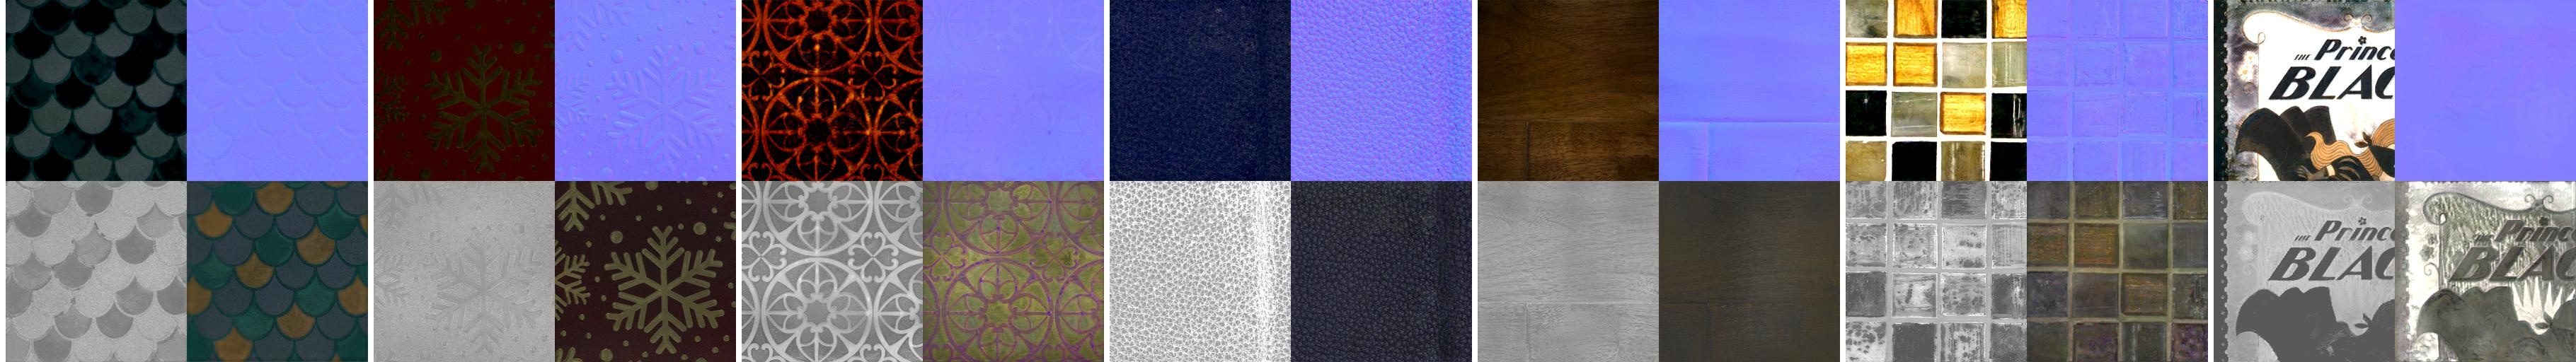
\includegraphics[width=\resLen]{svbrdf/teaser/maps.jpg}
	\end{tabular}
	\caption[Teaser]{\label{fig:svbrdf:teaser}
		We introduce a method to capture SVBRDF material maps from a small number of mobile flash photographs, achieving high quality results both on original and novel views. Our key innovation is optimization in the latent space of MaterialGAN, a generative model trained to produce plausible material maps; MaterialGAN thus serves as a powerful implicit prior for result realism. Here we show re-rendered views for several different materials under environment illumination. We use 7 inputs for these results (with 2 of them shown).
		(Please use Adobe Acrobat and click the renderings to see them animated.)
	}
\end{figure}

%\section{Introduction}
\label{sec:intro}
%
Despite a few decades of effort in computer graphics and vision, capturing spatially-varying reflectance of real-world materials remains a challenging and actively researched task.
Measurement methods have traditionally used custom hardware systems to densely sample illumination and viewing directions \cite{Marschner1999,Matusik2003}, followed by post-processing such as fitting parametric BRDF models \cite{Ngan2005}. However, such approaches are restricted to laboratory conditions.

Recent work has explored methods for casual capture of spatially-varying BRDFs (SVBRDFs) using commodity hardware and in less constrained environments \cite{Francken2009,Ren2011,Aittala2013,Aittala2015,Hui2017}.
These methods usually follow an \emph{inverse-rendering} approach: they define a forward rendering model and optimize reflectance parameters so that the simulated appearance matches physical measurements under certain image metrics.
With a small number of measured images, this approach is fundamentally under-constrained: there usually exist many material estimates capable of producing renderings that match the measurements, but
 many of these estimates can be unrealistic and may not generalize to novel illumination and viewing conditions.
The solution to this problem has been to \emph{regularize} the optimization using pre-determined \emph{material priors} such as linear low-dimensional BRDF models \cite{Ren2011,Hui2017} or stationary stochastic textures \cite{Aittala2015,Aittala2016}.
However, such hand-crafted priors do not generalize to a wide range of real-world materials.

More recently, learning-based approaches have demonstrated remarkable results for reconstructing SVBRDFs from one \cite{Deschaintre2018,Li2018} or more images \cite{Deschaintre2019}.
While these methods use rendering-based losses (similar to the inverse rendering approaches) during training, at test time they predict SVBRDFs from images using a single feed-forward pass through a deep network.
As a result, the reconstructed material parameters may not accurately reproduce the measured appearance.
In contrast, Gao et al. \shortcite{Gao2019} propose using an optimization-based approach in conjunction with a learned material prior.
Specifically, they train a fully-convolutional auto-encoder on a large material dataset and optimize in the latent space of this auto-encoder. This ensures that the reconstructed SVBRDF parameters both reproduce the measurements and are plausible real-world materials.
However, while this learned material prior is a significant improvement over hand-crafted priors, it still produces a relatively localized and highly flexible latent space that requires a good initialization (for example, from single image methods \cite{Deschaintre2018,Li2018}) and even then can fail to produce good results.

In this paper, we propose a different material prior that builds on the remarkable progress in image synthesis using deep Generative Adversarial Networks (GANs) \cite{Goodfellow2014,Karras2018,StyleGAN}.
We train \emph{MaterialGAN}---a StyleGAN2-based deep convolutional neural network \cite{StyleGAN2}---to generate plausible materials from a large-scale, spatially-varying material dataset \cite{Deschaintre2018}.
MaterialGAN learns \emph{global} correlations in material parameters, both spatially (thus encoding texture patterns) as well as across parameters (for example, relationships between diffuse and specular parameters).
As illustrated in Figure~\ref{fig:material_gan_samples}, sampling from the MaterialGAN latent space produces plausible, realistic materials with complex variations and diverse appearance.

While GANs have traditionally been used to synthesize images, we demonstrate a very different application, using MaterialGAN as a powerful prior in an inverse rendering-based material capture framework.
We append a rendering layer to MaterialGAN, setting up a differentiable pipeline from the learned latent space, through generating material maps, to rendering images under specified views and lighting.
This allows us to optimize the MaterialGAN latent vector(s) to minimize the error between the rendered and measured images and reconstruct the corresponding material maps.
Doing so ensures that the reconstructed SVBRDFs lie on the ``manifold of realistic materials'', while at the same time accurately reproducing the captured images.

%Additionally, we augment a standard per-pixel loss with a multi-resolution loss and a perceptual feature loss \cite{Johnson2016} based on a pre-trained VGG network \cite{VGG}.

We demonstrate that our GAN-based optimization framework produces high-quality SVBRDF reconstructions from a small number (3-7) images captured under flash illumination using hand-held mobile phones, and improves upon previous state-of-the-art methods \cite{Gao2019,Deschaintre2019}.
In particular, it produces cleaner, more realistic material maps that better reproduce the appearance of the captured material under both input \emph{and novel} lighting.
Moreover, as illustrated in Figure~\ref{fig:real}, MaterialGAN adapts to a wide range of SVBRDF samples ranging from diffuse to specular materials and near-stochastic textures to structured patterns with multiple distinct, complex materials.
%Finally, since our material prior does not make assumptions on the acquisition process, we can handle any arbitrary capture setup (for example different view or lighting conditions) without requiring any re-training. \KS{probably drop this since we are not actually showing this and this applies to Gao also.}

Furthermore, our GAN-based latent space offers the ability to edit the latent vector in semantically meaningful ways (via operations like interpolation in the latent space) and generate realistic materials that go beyond the captured images.
This is not possible with current material capture methods that do not afford any control over their per-pixel BRDF estimates.




%We optimize for an embedding of the unknown SVBRDF in several of the intermediate latent spaces of StyleGAN \cite{Abdal19a,Abdal19b}. Using a generative model to define the latent space may seem unnatural at first, as our goal is the capture of real data, not the generation of fake data. However, it turns out that a model trained to generate plausible SVBRDF map data can serve as a powerful implicit prior, keeping the optimization on the manifold of realistic results. Another important improvement is achieved by augmenting standard per-pixel image comparison with a multi-resolution comparison and with loss functions based on the feature maps of the VGG network \cite{VGG}. \milos{List of contributions?}

%For multi-image capture with co-located camera and light source (achieved in practice by multiple mobile phone flash photographs), we demonstrate results that succeed in the combined goals of matching the target images and producing plausible material maps, improving upon previous techniques \cite{Gao2019,Deschaintre2019}. Furthermore, our GAN-based latent space offers the additional ability to edit the latent vector to achieve semantically meaningful operations such as morphing.



%In this paper, we further explore the design of such a general framework for SVBRDF acquisition.
%Instead of end-to-end learning, we focus on an optimization-based \emph{analysis-by-synthesis} (also known as \emph{inverse-rendering}) approach that involves (i)~defining a forward appearance model; and (ii)~optimizing model parameters so that simulated appearances match physical measurements (under certain image metrics).
%In fact, analysis by synthesis is the foundation of many imaging techniques, and there has been a long history of previous methods taking this path \cite{Gardner2003,Aittala2013,Aittala2016,Gao2019}.

%Unfortunately, in the context of SVBRDF acquisition, no previous methods have been able to offer a sufficiently powerful prior on the manifold of realistic material maps, resorting instead to requiring many more measurements with very specific illumination patterns \cite{Gardner2003,Francken2009,Aittala2013}, restrictive assumptions on stationarity of textures \cite{Aittala2016} or initialization with a different method \cite{Gao2019}.

%More recently, a family of deep-learning-based methods have been introduced and are capable of significantly reducing the number of input images required, sometimes down to as low as one.
%These methods leverage neural networks to define loss functions, latent spaces, or to learn parameter inference pipelines end-to-end.

%Prior works have shown that a single image generally carries insufficient information for accurately recovering SVBRDFs, regardless of the algorithm used.
%On the other hand, a few recent works~\cite{Gao2019,Deschaintre2019} have demonstrated the possibility for further progress (that offers a good balance between acquisition cost and reconstruction quality) by instead capturing a small number of images followed by a robust reconstruction leveraging neural priors.
%However, within this space, there are still a large number of design options, such as acquisition configurations (e.g., illumination patterns) and reconstruction techniques, that remain to be explored.

%A main challenge for solving analysis-by-synthesis optimizations is the under-constrained nature of these problems.
%With a small number of measured images, there usually exist many material model parameters capable of producing renderings that match the measurements.
%Most of these solutions, unfortunately, have unrealistic parameter textures and cannot generalize to novel illumination and viewing conditions.
%To address this problem, the general solution is to \emph{regularize} the optimization using pre-determined \emph{priors}.
%Unfortunately, in the context of SVBRDF acquisition, no previous methods have been able to offer a sufficiently powerful prior on the manifold of realistic material maps, resorting instead to requiring many more measurements with very specific illumination patterns \cite{Gardner2003,Francken2009,Aittala2013}, restrictive assumptions on stationarity of textures \cite{Aittala2016} or initialization with a different method \cite{Gao2019}.

%In this paper, we take a step forward by solving the analysis-by-synthesis optimization in the latent space of a generative model, specifically StyleGAN \cite{StyleGAN}, trained to generate plausible SVBRDF maps.
%We optimize for an embedding of the unknown SVBRDF in several of the intermediate latent spaces of StyleGAN \cite{Abdal19a,Abdal19b}. Using a generative model to define the latent space may seem unnatural at first, as our goal is the capture of real data, not the generation of fake data. However, it turns out that a model trained to generate plausible SVBRDF map data can serve as a powerful implicit prior, keeping the optimization on the manifold of realistic results. Another important improvement is achieved by augmenting standard per-pixel image comparison with a multi-resolution comparison and with loss functions based on the feature maps of the VGG network \cite{VGG}. \milos{List of contributions?}

%For multi-image capture with co-located camera and light source (achieved in practice by multiple mobile phone flash photographs), we demonstrate results that succeed in the combined goals of matching the target images and producing plausible material maps, improving upon previous techniques \cite{Gao2019,Deschaintre2019}. Furthermore, our GAN-based latent space offers the additional ability to edit the latent vector to achieve semantically meaningful operations such as morphing.

% On synthetic data, we also show that our latent space optimization applies to other illumination configurations, such as pattern projection with an LCD screen. \gy{TODO:}

%\section{Related work}
\label{sec:related}

\paragraph{Reflectance capture.}
\revision{Acquiring} material data from physical measurements is the goal of a broad range of methods.
\revision{Please refer to surveys~\cite{weyrich09,Guarnera2016,dong19} for more comprehensive introduction to the related works.}

Most \revision{reflectance capture} approaches %generally
observe a material sample under \revision{varying viewing} and lighting configurations. They differ in the number of light patterns required and their \revision{types such as} moving linear light \cite{Gardner2003,Ren2011}, Gray code patterns \cite{Francken2009}, spherical harmonic illumination \cite{Ghosh2009}, and Fourier patterns \cite{Aittala2013}.

Methods have also been proposed for material capture ``in the wild'', i.e., under uncontrolled environment conditions with commodity hardware, typically captured with a hand-held mobile phone with flash illumination. Some of these methods impose strong priors on the materials, such as linear combinations of basis BRDFs \cite{Hui2017,Xu2016} (where the basis BRDFs can come from the measured data \cite{Matusik2003}). Later work by Aittala et al. \shortcite{Aittala2015,Aittala2016} estimated per-pixel parameters of stationary spatially-varying SVBRDFs from two-shot and one-shot photographs.
In the latter case, the approach used a neural Gram-matrix texture descriptor based on the texture synthesis and feature transfer work of Gatys \shortcite{Gatys2015,Gatys2016} to compare renderings with similar texture patterns but without pixel alignment.

More recently, deep learning-based approaches have demonstrated remarkable progress in the quality of SVBRDF estimates from single images (usually captured under flash illumination) \cite{Li2017,Deschaintre2018,Li2018}. These methods train deep convolutional neural networks with large datasets of artistically created SVBRDFs, and with a combination of losses that evaluate the difference in material maps and renderings from the dataset ground truth.

Deschaintre \shortcite{Deschaintre2019} extended the single-shot approach to multiple images. The key idea is to extract features from the input images with a shared encoder, max-pooling the features and decoding the final maps from the pooled features. This architecture has the benefit of being independent of the number of inputs, while also not requiring explicit light position information. In our experience, this approach produces smooth, plausible maps with low artifacts; however, re-rendering the maps tends to be not as close to the target measurements because the network cannot ``check'' its results at runtime. Moreover, we find that especially on real data, this method also has strong biases such as dark diffuse albedo maps and exaggerating surface normals (especially along strong image gradients that might be caused by albedo variations). We believe this is not due to any technical flaw; the method may be reaching the limit of what is possible using current feed-forward convolutional architectures and currently available datasets.

Gao et al. \shortcite{Gao2019} introduced an inverse rendering-based material capture approach that optimizes for material maps to minimize error with respect to the captured images. Since this is an under-constrained problem, they propose optimizing over the latent space of a learned material auto-encoder network to minimize rendering error. This approach has the benefit of explicitly matching the appearance of the captured image measurements, while also using the auto-encoder as a material ``prior''. Moreover, the encoder and decoder are fully convolutional, which has the advantage of resolution independence.
However, we find that the convolutional nature of this model also has the disadvantage of only providing local regularization and not capturing global patterns in the material, such as the long-range spatial patterns and correlations between the different material parameter maps. As a result, this method relies on previous methods (for example, Deschaintre et al.~\shortcite{Deschaintre2018}) to provide a good initialization, without which it can converge to poor results.
%Thus this approach provides only local regularization (even though it is an improvement compared to conventional optimization directly in pixel space), and generally needs to be initialized with the result of another method, providing further cleanup.
In contrast, our MaterialGAN is a more globally robust latent space and produces higher quality reconstructions without requiring accurate initializations, though it is no longer resolution-independent.

\paragraph{Generative adversarial networks.}
GANs~\cite{GAN} have become extremely successful in the past few years in various domains, including images~\cite{DCGAN}, video~\cite{Tulyakov18}, audio~\cite{Donahue18}, \revision{and 3D shapes~\cite{Li19}}. A GAN typically consists of two competing networks; a generator, whose goal is to produce results that are indistinguishable from the real data distribution, and a discriminator, whose job is to learn to identify generated results from real ones. For generating realistic images (especially of human faces), there has been a sequence of improved models and training strategies, including ProgressiveGAN~\cite{Karras2018}, StyleGAN~\shortcite{StyleGAN} and StyleGAN2~\shortcite{StyleGAN2}. StyleGAN2 in particular is the state-of-the-art GAN model and our work is based on its architecture, modified to output more channels.

\revision{Recently, GANs have also been used to solve inverse problems \cite{Bora17,Asim19,Malley19}.}
%Recent research in the GAN space has also focused
\revision{In computer graphics and vision, this work has focused} on embedding images into the latent space, with the goal of editing the images in semantically meaningful ways via latent vector manipulations \cite{Zhu2016}. This embedding requires solving an optimization problem to find the latent vector.
%Among the first papers to consider embedding images into a GAN latent space, for the purposes of editing them while staying on the learned manifold, was the approach by Zhu et al. \shortcite{Zhu2016}.
%Furthermore, the embedding needs to be ``soft'', and robust to the fact that the model may not be able generate pixel-aligned results. These considerations make the link between generative modeling and our material capture application more clear.
More recent work such as Image2StyleGAN~\cite{Abdal19a} and Image2StyleGAN++~\cite{Abdal19b} has looked at problem of embedding images specifically into the the StyleGAN latent space. While these methods focus on projecting portrait images into face-specific StyleGAN models, we find their analysis can be adapted to our problem.
We build on this to propose a GAN embedding-based inverse rendering approach.
%To our knowledge, none of the previous work on GANs has used them to solve the problem of under-constrained optimization within an analysis-by-synthesis framework.



% We instead train a generator model for SVBRDF maps $\albedo$, $\normal$ and $\rough$, by training on a large dataset of such maps. Then, instead of embedding given SVBRDF maps into the space (which we can also do, but is less useful), we use the learned generator as the decoder in eq. \ref{eq:opt2}. We find the loss function design is also a key component of the problem: a weighted combination of pixel losses at different resolutions, combined with several VGG feature maps losses, leads to a massively improved result over using a simple per-pixel loss.



%\section{MaterialGAN: A Generative SVBRDF Model}
\label{sec:svbrdf:gan}

Generative Adversarial Networks \cite{goodfellow2014generative} are trained to map an input from a latent space (often randomly sampled from a multi-variate normal distribution) to a plausible instance of the target distribution.
In recent years, GANs have made remarkable progress in synthesizing high-resolution, photo-realistic images. Inspired by this progress, we propose MaterialGAN, a GAN that is trained to generate plausible materials, thus implicitly learning an SVBRDF manifold. MaterialGAN is based on the architecture of StyleGAN2 \cite{karras2020analyzing}.


\subsection{Overview of StyleGAN and its latent spaces}
\label{ssec:latent_space}

StyleGAN2 \cite{karras2020analyzing} is an improvement of StyleGAN \cite{karras2019style} and is the state-of-the-art generative adversarial network (GAN) for image synthesis, especially for human faces.
The architecture has several advantages over previous models like ProgressiveGAN \cite{karras2018progressive} and DCGAN \cite{radford2015unsupervised}. For our purposes, the main advantage is that the model is not simply a black-box stack of convolution and upsampling layers, but has additional, more specific structure, allowing for much easier inversion (latent space optimization).
The StyleGAN2 architecture starts with a learned constant $4 \times 4 \times 512$ tensor and progressively upsamples it to the final output target resolution via a sequence of convolutional and upsampling layers (7 in total to end with a final image resolution of $256 \times 256$).
Given an input latent code vector $\bmz \in \calZ \subset \bbR^{512}$, StyleGAN2 transforms it through a non-linear mapping network of fully-connected layers into an intermediate latent vector $\bmw \in \calW \subset \bbR^{512}$.
The rationale for the introduction of the space of~$\calW$ is that while $\calZ$ requires (almost) every latent $\bmz \in \calZ$ to correspond to a realistic output, vectors $\bmw \in \calW$ are free from this overly stringent constraint, which leads to a less ``entangled'' mapping, with more meaningful dimensions (see \cite{karras2019style,karras2020analyzing} for more discussion).
In the original StyleGAN, the vector $\bmw \in \calW$ is mapped via a learned affine transformation to mean and variance ``style'' vectors that control adaptive instance normalizations (AdaIN) \cite{huang2017arbitrary} that are applied before and after every convolution in the generation process (thus $7 \times 2 = 14$ times for a model of resolution $256 \times 256$). The statistics of the AdaIN normalizations caused the feature maps and output images of StyleGAN to suffer from droplet artifacts. StyleGAN2 removes the droplet artifacts entirely by replacing the AdaIn normalization layers with a demodulation operation which bakes the entire style block into a single layer while maintaining the same scale-specific control as StyleGAN.
We construct a matrix $\bmw^+ \in \calW^+ \subset \bbR^{512 \times 14}$ by replicating $\bmw$ 14 times.
During training and standard synthesis, the columns of $\bmw^+$ are identical, and correspond to $\bmw$.
However, as we will discuss later (and similar to Abdal et al. \cite{abdal2019image2stylegan}), we relax this constraint when optimizing for an embedding; $\calW^+$ thus becomes an extended latent space, more powerful than $\calW$ or $\calZ$.
Additionally, StyleGAN2 injects Gaussian noise, $\bmxi$, into each of the 14 layers of the generator.
This noise gives StyleGAN2 the ability to synthesize stochastic details at multiple resolutions.
Abdal et al. \cite{abdal2020image2stylegan++} make the observation that one can also treat these noise inputs $\bmxi$ as a latent space $\calN$. Thus, combining these two spaces defines yet another latent space $\calWN$.


\subsection{MaterialGAN training}
\label{ssec:training}

MaterialGAN was trained with the dataset provided by Deschaintre et al. \cite{deschaintre2018single} (and also used in Gao et al. \cite{gao2019deep}). They generated this dataset by sampling the parameters of procedural material graphs from Allegorithmic Substance Share to create an initial set of 155 high-quality SVBRDFs at resolution $4096 \times 4096$. The dataset was augmented by blending multiple SVBRDFs and generating $256 \times 256$ resolution crops at random positions, scales and rotations. The final dataset consists of around 200,000 SVBRDFs. For detailed information about the curation of dataset we refer the reader to \cite{deschaintre2018single}. Since pairs of SVBRDFs in the dataset were the same with only a slight variation, we selected 100,000 SVBRDFs.
The maps for each SVBRDF are stacked in 9 channels (3 for albedo, 2 for normals, 1 for roughness, and 3 for specular albedo). We account for this by adapting the MaterialGAN architecture to output 9-channel outputs. MaterialGAN is trained in TensorFlow (version 1.15) with the same loss functions and similar hyper-parameters from StyleGAN2 \cite{karras2020analyzing}. StyleGAN2 configuration F was used for all experiments. The generator and discriminator were trained using Adam optimizers. The learning rate was increased per resolution from 0.001 to 0.0025 for both the generator and the discriminator. The discriminator was shown 25 million images. Training on 8$\times$ Nvidia Tesla V100 takes about 5 days.
Figure \ref{fig:svbrdf:matgan} shows materials generated by randomly sampling the MaterialGAN latent space and images rendered from them. As can be seen here, MaterialGAN generates a wide variety of nearly photorealistic materials ranging from structured to stochastic, diffuse to specular, and with large-scale variations to fine detail. Furthermore, Figure \ref{fig:svbrdf:morph_fake} and the accompanying video show example interpolations between pairs of generated materials in the latent space, producing plausible non-linear morphing results.

\input{tex/svbrdf/fig/morph_fake}

%\section{SVBRDF Capture using MaterialGAN}
\label{sec:svbrdf:framework}

\input{tex/svbrdf/fig/framework}

We utilize MaterialGAN, the powerful generative model described in the previous section, in a fundamentally new fashion: to \emph{capture} SVBRDF maps.
Specifically, we use MaterialGAN as a \emph{material prior} for SVBRDF acquisition via an inverse rendering framework (See Figure. \ref{fig:svbrdf:framework}).
Our goal is to estimate the SVBRDF parameter maps from one or a small number of photographs of a near-planar material sample.
We utilize a common BRDF model that involves a diffuse and a specular component using the microfacet BRDF with the GGX normal distributions \cite{Walter07}.
Our unknown parameter vectors $\params := (\albedo,\normal,\rough,\spec)$ encode the four per-pixel parameter maps: diffuse albedo $\albedo$, surface normal $\normal$, roughness $\rough$, and specular albedo $\spec$.
To recover the unknown parameter maps, we capture $k$ images $\image_1, \cdots, \image_k$.
We assume known viewing and lighting configurations for each image, which we denote as $(\light_i, \camera_i)$.
Further, we assume that the material is lit by a single point source, collocated with the camera.
\footnote{
	In theory, non-collocated lights, area lights or projection patterns (e.g. on an LCD or similar screen) can be used as well, and would require a straightforward modification to our forward rendering process.
}
The images can be reprojected into a common frontal view (which is straightforward with a known viewing configuration).

We introduce a differentiable rendering operator $\render$ that takes as input the parameter maps as well as the viewing and lighting configurations, and synthesizes corresponding images of the material.
Under this setup, our goal is to find values of the unknown parameters $\params$ so that renderings with these parameters match the measurements $\image_i$.
In other words, we focus on solving the following optimization problem:
\begin{equation}
	\label{eq:opt1}
	\paramsopt = \textstyle\argmin_{\albedo, \normal, \rough} \sum_{i=1}^k \loss(\render(\params; \,\light_i, \camera_i), \image_i),
\end{equation}
where $\loss$ is a loss function that measures the difference between the captured images, $\image_i$ and the renderings generated from the estimated SVBRDF parameters, $\render(\params; \,\light_i, \camera_i)$.


\subsection{Incorporating the MaterialGAN prior}

Eq. \eqref{eq:opt1} is, in general, a challenging optimization to solve due to its under-constrained nature.
Given a small number of input measurements, the optimization can overfit to the input, producing implausible maps that do not generalize to novel views and lighting.
To overcome this challenge, we leverage the MaterialGAN prior: instead of directly optimizing for the parameter maps $\params$,  we can optimize for a vector $\latent$ in the MaterialGAN \emph{latent space} and map (decode) this latent vector back into material maps $\params$.
The optimization problem then becomes:
\begin{equation}
	\label{eq:opt_gan}
	\latentopt = \textstyle\argmin_{\latent} \sum_{i=1}^k \loss(\render(\generator(\latent); \,\light_i, \camera_i), \image_i),
\end{equation}
where $\generator$ is the learned MaterialGAN generator.
Given that both $\generator$ and $\render$ are differentiable operations, Eq. \eqref{eq:opt_gan} can be optimized via gradient-based methods to estimate $\latentopt$ and the corresponding SVBRDF maps $\generator(\latentopt)$.

The above operation is similar to recent work on embedding images in the StyleGAN latent space \cite{Abdal19a,Abdal19b}.
The key difference is that we do not match material parameters directly, but evaluate their error through the rendering operator $\render(\cdot)$.
To our knowledge, ours is the first approach to use a GAN latent space in combination with a rendering operator.


\paragraph{Loss function.}
We optimize Eq. \ref{eq:opt_gan} using a combination of a standard per-pixel L2 loss and a ``perceptual loss'' \cite{Johnson2016} that has been shown to produce sharper results in image synthesis tasks:
\begin{equation}
	\label{eq:loss}
	\loss(\image, \image') = \lambda_1 \lossPix + \lambda_2 \lossPercp,
\end{equation}
The perceptual loss is defined as:
\begin{equation}
	\lossPercp(\image, \image') = \textstyle\sum_{j=1}^4 w^\mathrm{percept}_j \left\|F_j(\image) - F_j(\image')\right\|_2^2,
\end{equation}
where $F_1, \cdots, F_4$ are the flattened feature maps corresponding to the outputs of VGG-19 layers  \texttt{conv1\_1}, \texttt{conv1\_2}, \texttt{conv3\_2}, and \texttt{conv4\_2} from a pre-trained VGG network \cite{VGG}. See section \ref{ssec:optim} for more details.


\paragraph{Optimization details.}
We convert the TensorFlow-trained MaterialGAN model to PyTorch, in which our optimization framework is implemented. We optimize Eq. \ref{eq:opt_gan} using the Adam optimizer in PyTorch, with a learning rate of $0.01$. We set all other hyper-parameters to default values.
Now that our basic optimization framework is set up, there remain two key ingredients to implement our GAN-based optimization framework (Eq. \eqref{eq:opt_gan}): (i)~the choice of \emph{latent space} that we optimize $\latent$ over, and (ii)~our optimization strategy to minimize the objective function. In the following sections, we describe our approach, along with an empirical analysis of these design choices.


\subsection{Latent space}
\label{ssec:latent}

As discussed in Sec. \ref{ssec:latent_space}, StyleGAN2 (and consequently, MaterialGAN) has a number of potential latent spaces.
In particular, MaterialGAN uses three different \emph{style} latent spaces: the input latent code $\bz \in \calZ$ , the intermediate latent code $\bw \in \calW$ and per-layer styles $\bw^+ \in \calW^+$.
StyleGAN2 also injects noise $\noise \in \calN$ into every layer of the network to generate stochastic variations.
The typical forward generation process of the GAN only uses $\bz$, with $\bw$ being generated from $\bz$ via a mapping network, and $\bw^+$ being generated from $\bw$ via affine transformations.
However, Abdal~et~al. \cite{Abdal19a} note that the space of $\calZ$ is too restrictive for accurate embedding of faces or other content into the GAN space.
In other words, given the image of a human face, it is generally impossible to find a single $\bz \in \calZ$ such that the generated image closely matches the target.
This remains the case even when extending the space to $\calW$, i.e., when searching for a $\bw$ instead of a $\bz$.
The space $\calW^+$, on the other hand, offers much stronger representative power.
Our experiments on embedding material maps into MaterialGAN demonstrate that optimizing for $\calW^+$ is also needed for MaterialGAN to accurately reproduce input maps.
We demonstrate this in Figure \ref{fig:svbrdf:embed}, via an experiment where we embed a given material (with known material maps) into MaterialGAN.
As shown in rows (2) and (3), maps generated by optimizing $\bw^+ \in \calW^+$ contain more detail compared to those using $\bw \in \calW$.

\input{tex/svbrdf/fig/embed}

On the other hand, some small-scale details are still missing.
In fact, according to our experiments, only colors and large-scale features can be captured by the $\calW^+$ space.
For depicting high-frequency patterns, as demonstrated in rows (4) and (5) of Figure \ref{fig:svbrdf:embed}, we need to go even further and optimize the noise vector $\noise$ (instead of drawing it from multi-variate normal distributions).
We note that optimizing for the noise component is even more important in MaterialGAN, compared to embedding faces in StyleGAN or StyleGAN2.
We suspect that this is because with human faces, the distinction between large-scale features (e.g., eyes, noise, and mouth) and small-scale features (e.g., winkles) is very prominent, allowing the $\calW^+$ space to focus mostly on the large-scale features while leaving the small-scale ones to the noise vector $\noise \in \calN$.
In our case, the boundary between large-scale and small-scale material features is much less distinct.
The physical scales of real-world materials varies in a continuous fashion, making it virtually impossible to assign them to only one of the $\calW^+$ and $\calN$ spaces.
We hypothesize that for this reason, we need to focus on both $\calW^+$ and $\calN$ to achieve high-quality reconstruction of SVBRDF maps.
Based on these empirical observations, estimating SVBRDF parameter maps from photographs using our pre-trained MaterialGAN boils down to solving the following optimization:
\begin{equation}
	\latentopt = \argmin_{\bw^+ \in \calW^+,\, \noise \in \calN} \sum_{i=1}^k \loss(\render(\generator(\bw^+, \noise); \,\light_i, \camera_i), \image_i).
\end{equation}
Since there are two variables $\bw^+$ and $\noise$ that behave in a correlated fashion, a proper optimization strategy is crucial to achieve high-quality results. We now discuss our alternating two-step optimization method.

\subsection{Optimization strategy}
\label{ssec:optim}

Abdal~et~al. \cite{Abdal19a,Abdal19b} recommended using a two-stage setting by first optimizing $\bw^+$ (with $\noise$ fixed) and then $\noise$ (with $\bw^+$ fixed).
In our case, this approach does work in some cases but is not always the top-performing option.
In addition to this strategy, we propose two alternatives, leading to three different optimization schemes:
\begin{enumerate}
	\item \textbf{Strategy 1}: Optimize $\bw^+$ first, then optimize $\noise$;
	\item \textbf{Strategy 2}: Jointly optimize both $\bw^+$ and $\noise$;
	\item \textbf{Strategy 3}: Alternatively optimize $\bw^+$ and $\noise$ for a small number (for example, 10) of iterations each.
\end{enumerate}

\input{tex/svbrdf/fig/strategy}

Figure \ref{fig:svbrdf:strategy} shows a comparison of these strategies.
All of them give reasonable results, but Strategy 1 is better suited for materials with strong large-scale features.
Strategy 2 provides the fastest convergence because it allows the noise vector $\noise$ to be modified from the very beginning.
This, however, generally causes the optimization to use $\noise$ for encoding higher-level features and is prone to overfitting.
Finally, Strategy 3---a hybrid of Strategies 1 and 2---behaves in a more robust fashion than either of the previous strategies in most cases.
We use Strategy 3 for all the results in our paper.
Additionally, our experiments indicate that it is desirable to use different VGG layer weights for the optimization of $\bw^+$ and $\noise$. The weights we are using are, for $\bw^+$: [1/512,1/512,1/128,1/64]; for $\noise$: [1/64,1/64,1/256,1/512].


\input{tex/svbrdf/fig/noise_vs_refine}

\paragraph{Noise optimization vs. post-refinement.}
\label{ssec:post-refine}
Instead of optimizing latent space $\bw^+$ with noise $\noise$, another option is to apply post-refinement (that is, pixel-space optimization without any latent space) after optimizing $\bw^+$ only. However, the space $\bw^+$ is too small to realistically match per-pixel detail: if optimizing $\bw^+$ only, the resulting maps have significant artifacts. Adding post-refinement to such a result essentially becomes per-pixel optimization (with little regularization), which tends to to work poorly with a small number of inputs. Optimizing $\noise$ offers more powerful regularization, as the noise is inserted into all layers of the generator, rather than just appended at the end (like post-refinement). We show two failure examples in Figure \ref{fig:svbrdf:noise_vs_refine}, where optimizing $\bw^+$ leads to unsatisfactory texture maps.


\subsection{Initialization}
\label{ssec:init}

\input{tex/svbrdf/fig/init}

We find that our method is robust to the initialization of the latent vectors. We experimented with using the same initial configuration---represented by the material produced by the mean $\bw$ of our GAN training data (see Figure \ref{fig:svbrdf:init}(a))---and found that is works well for most of the materials we tried (both synthetic and real).
However, this initialization represents a material with a high roughness (reflecting a bias in our training data) and sometimes leads to errors when fitting highly specular / low roughness materials.
Therefore, we add an additional low roughness initialization (see Figure \ref{fig:svbrdf:init}(b)).
In practice, given the captured images, we run our MaterialGAN optimization starting from both initializations and retain the result with the lowest optimization error of Eq. \eqref{eq:loss}.
All of our results in this paper followed this scheme.


%\section{Results}
\label{sec:svbrdf:results}

\textbf{(Only a small subset of our results fits into the thesis. Please see our supplemental material and video for more results.
[\href{https://www.ics.uci.edu/~yug10/webpage/suppl/2020TOG/index.html}{Click here}])}

\paragraph{Test data.}
For synthetic tests, we use several examples from the test set of Deschaintre \cite{deschaintre2018single}, as well as some from the Adobe Stock dataset \cite{li2018materials}. This gives a total of 30 synthetic results.
For our real results, we use a hand-held mobile phone to capture images with flash, resulting in a collocated camera and point light illumination.
Similar to previous work \cite{hui2017reflectance,deschaintre2019flexible}, we use a paper frame to register the multiple images.
We add markers to the frame to improve camera pose estimation.
Using this process, we capture 40 physical samples with nine images per material, roughly covering the sample with $3 \times 3$ specular highlights. 
Unless otherwise specified, all our results use seven images for inverse-rendering optimizations and the remaining two (under novel lighting) for evaluating the results.

\paragraph{Inverse-rendering performance.}
Our optimization takes about 2 minutes to complete 2000 iterations on a Titan RTX GPU. In many cases, the results converge after ~500 iterations, but we use 2000 everywhere for simplicity.

\input{tex/svbrdf/fig/synthetic}

\paragraph{Testing on synthetic data.}
Figure \ref{fig:svbrdf:synthetic} contains two synthetic results using our method, showing a close match both in maps and in novel view renderings. For more results, please refer to supplemental materials. We note that all methods perform better on synthetic data than on real data, possibly because of the exact BRDF model match and perfect calibration, and also
because the synthetic test set, while distinct from the training set, is relatively similar in style.

\input{tex/svbrdf/fig/real}

\subsection{Comparison with prior work on real data}
\label{ssec:real}

\input{tex/svbrdf/tab/accuracy}

Here we compare our method and Gao et al. \cite{gao2019deep}. For more results and comparisons, including with Deschaintre et al. \cite{deschaintre2019flexible}, and including with and without initialization for ours and Gao's method, please refer to supplemental materials.
We show 10 real examples from our cell phone capture pipeline in Figure \ref{fig:svbrdf:real}. Note that Gao's method is significantly dependent on initialization, while the same is not true for our method. Therefore, in this figure, we show Gao's result \emph{with initialization} by Deschaintre et al. \cite{deschaintre2019flexible}, while our result is shown \emph{without initialization}.
Furthermore, note that we are initializing Gao's method with the 2019 multi-input method by Deschaintre, which is a better initialization than the 2018 single-input method. Thus the baseline we are comparing against is, strictly speaking, even higher than what is published in Gao et al., and combines the two best methods published at this time.
Generally, we find that our method produces cleaner maps and is less prone to overfitting (burn-in) than Gao's, while producing more accurate re-renderings under original and novel lighting. Table \ref{tab:svbrdf:accuracy} shows a quantitative evaluation of the re-rendering quality on novel lighting. As these novel views would be hard to match pixel-wise using any method, as they have never been observed, we use a perceptual method, specifically the Learned Perceptual Image Patch Similarity (LPIPS) metric \cite{zhang2018unreasonable} (lower is better). Note that our method (without initialization by Deschaintre's method) produces better scores for novel views than Gao's method (with initialization) for most images; even in the case where our LPIPS score is worse, our maps still look more plausible overall.
We also report quantitative evaluations (histograms) for our entire set of results (see Figure \ref{fig:svbrdf:rmse}). For synthetic data, we compare the RMSE of all predicted maps (diffuse albedo, normal, roughness, specular albedo), as we do know the ground truth for them. For both synthetic and real data, we compare the LPIPS scores on novel lighting. We use a + sign to indicate initialization by Deschaintre et al. In the top row, we compare both methods without initialization by Deschaintre's method, while in the middle row, both methods are initialized, and in the bottom row, we compare our method without initialization to Gao's with initialization. Generally, we find that if both methods are initialized the same way, our method outperforms Gao's. Even in the last row, our performance is comparable on synthetic data (worse on normal map and better on diffuse/specular maps) and still better on real data overall.

\input{tex/svbrdf/fig/rmse}

\paragraph{Note about Deschaintre et al.}
We find that the results from \cite{deschaintre2019flexible} have much less accurate re-rendering than either ours or Gao's method, as they are not doing any optimization to precisely fit the target images. The mismatches we observe are definitely not due to simple scaling or gamma correction issues, as that would be consistent across examples; rather, we find that the method performs much better on synthetic examples that match the visual style of its training set. On the other hand, their method is fast and results tend to be clean and artifact-free, so they are very suitable for initialization of optimization methods.


\subsection{Additional comparisons}

\input{tex/svbrdf/fig/diff_init}

\paragraph{Optimization with different initializations.}
In Figure \ref{fig:svbrdf:diff_init}, we compare our method to Gao's with and without initialization by Deschaintre's method in all 4 combinations, on a synthetic and a real example. This shows that Gao's method more significantly dependent on good initialization that ours (even though our method can still occasionally benefit).

\input{tex/svbrdf/fig/refine}

\paragraph{Post-refinement.}
In general, the quality of our maps is sufficient after using our MaterialGAN based optimization. However, Gao's method introduced a post-refinement step, where the maps are further optimized without any latent space, and with at most minor regularization. Therefore, we also implement a similar post-refinement step. However, like good initialization, this post-refinement makes less of a difference in our method, and Gao's method is more dependent on it, as it produces significantly blurry maps without it. This is shown in Figure \ref{fig:svbrdf:refine}; note the difference in sharpness of the maps.

\input{tex/svbrdf/fig/multi_fake}

\paragraph{Optimization with different numbers of input images.} While most of our results are shown with 7 inputs, using two additional inputs for novel lighting evaluation, our method does work with various numbers of input images. We show 3 synthetic examples in Figure \ref{fig:svbrdf:multi_fake}, with different numbers of inputs from 1 to 25. All the three examples are the same as used in Gao's work. The errors of both reconstructed SVBRDF maps and novel-view renderings generally decrease with more input images, as is expected for an inverse-rendering method. In Figure \ref{fig:svbrdf:multi_real}, we compare real capture results with 1, 3, and 7 inputs, with and without initialization by Deschaintre's method, and also include Gao's results for 3 and 7 inputs (with initialization). Our result remains plausible with 3 inputs, though artifacts do get reduced with more inputs. For all numbers of inputs, our result (with or without initialization) tends to be cleaner than Gao's.

\input{tex/svbrdf/fig/multi_real}

\paragraph{Editing operations.} An additional advantage of the StyleGAN-based latent space is the ability to achieve semantically meaningful operations such as morphing, by interpolating two or more parent latent codes to create a hybrid offspring material. Morphing in latent space often preserves semantic features qualitatively better than naive interpolation in pixel space. Figure \ref{fig:svbrdf:morph_real} and the supplemental video show morphing of a few real materials using linear interpolation in latent space, compared to the corresponding naive interpolation (linear in pixel space).

\input{tex/svbrdf/fig/morph_real}

%\section{Conclusion and Future Work}
\label{sec:conclusion}
%
\paragraph{Discussion and limitations.}
While we believe our framework improves upon the state of the art, there are also some limitations. Our current BRDF model is shared by previous work, but certain common effects (layering on book covers, subsurface fiber scattering in woods, anisotropy in fabrics) are not correctly captured by it. An extension of our generative model and rendering operator would be possible, though the key challenge is finding high-quality  training data for these effects.

Our assumption of almost flat samples will fail for materials with strong relief patterns, and will produce blurring or ghosting if there are obvious parallax effects in the aligned captured images. Strong self-shadowing or inter-reflections are also not currently handled. Solving for height instead of normal, with a more advanced rendering operator, may be able to resolve parallax effects \revision{and to} correctly predict (and undo) shadowing effects from strong height variations.

Furthermore, more precise calibration may improve our accuracycd. This would likely require knowledge of the cell phone hardware, and/or pre-calibration of its properties (e.g. flash light falloff, lens vignetting, and color processing properties).

%\revision{The resolution of our result can be increased with a coarse-to-fine post-process, since we have a fairly good result as the initialization of next level of resolution.}

\paragraph{Conclusion.}
We propose a novel method for acquiring SVBRDFs from a small number of input images, typically 3 to 7, captured using a hand-held mobile phone.
We use an optimization framework that leverages a powerful material prior, based on a generative network, MaterialGAN, trained to synthesize plausible SVBRDFs.
MaterialGAN learns correlations in SVBRDF parameters and provides local and global regularization to our optimization.
This produces high-quality SVBRDFs that accurately reconstruct the input images, and because of our MaterialGAN prior, lie on a plausible material manifold.
As a result, our reconstructions generalize better to novel views and lighting than previous state-of-the-art methods.

We believe that our work is only a first step toward GAN-based material analysis and synthesis and our experiments suggest many avenues for further exploration including improving material latent spaces and optimization techniques using novel architectures and losses, learning disentangled and editable latent spaces, and expanding beyond our current isotropic BRDF model.





\chapter{Inverse Rendering for Microscale Material Parameters}
\label{cpt:bayesian}

\begin{figure}[h!]
	\centering
	\setlength{\resLen}{.875in}
	\setlength{\raiseLen}{.1in}
	\addtolength{\tabcolsep}{-5pt}
	\vspace{-30pt}
	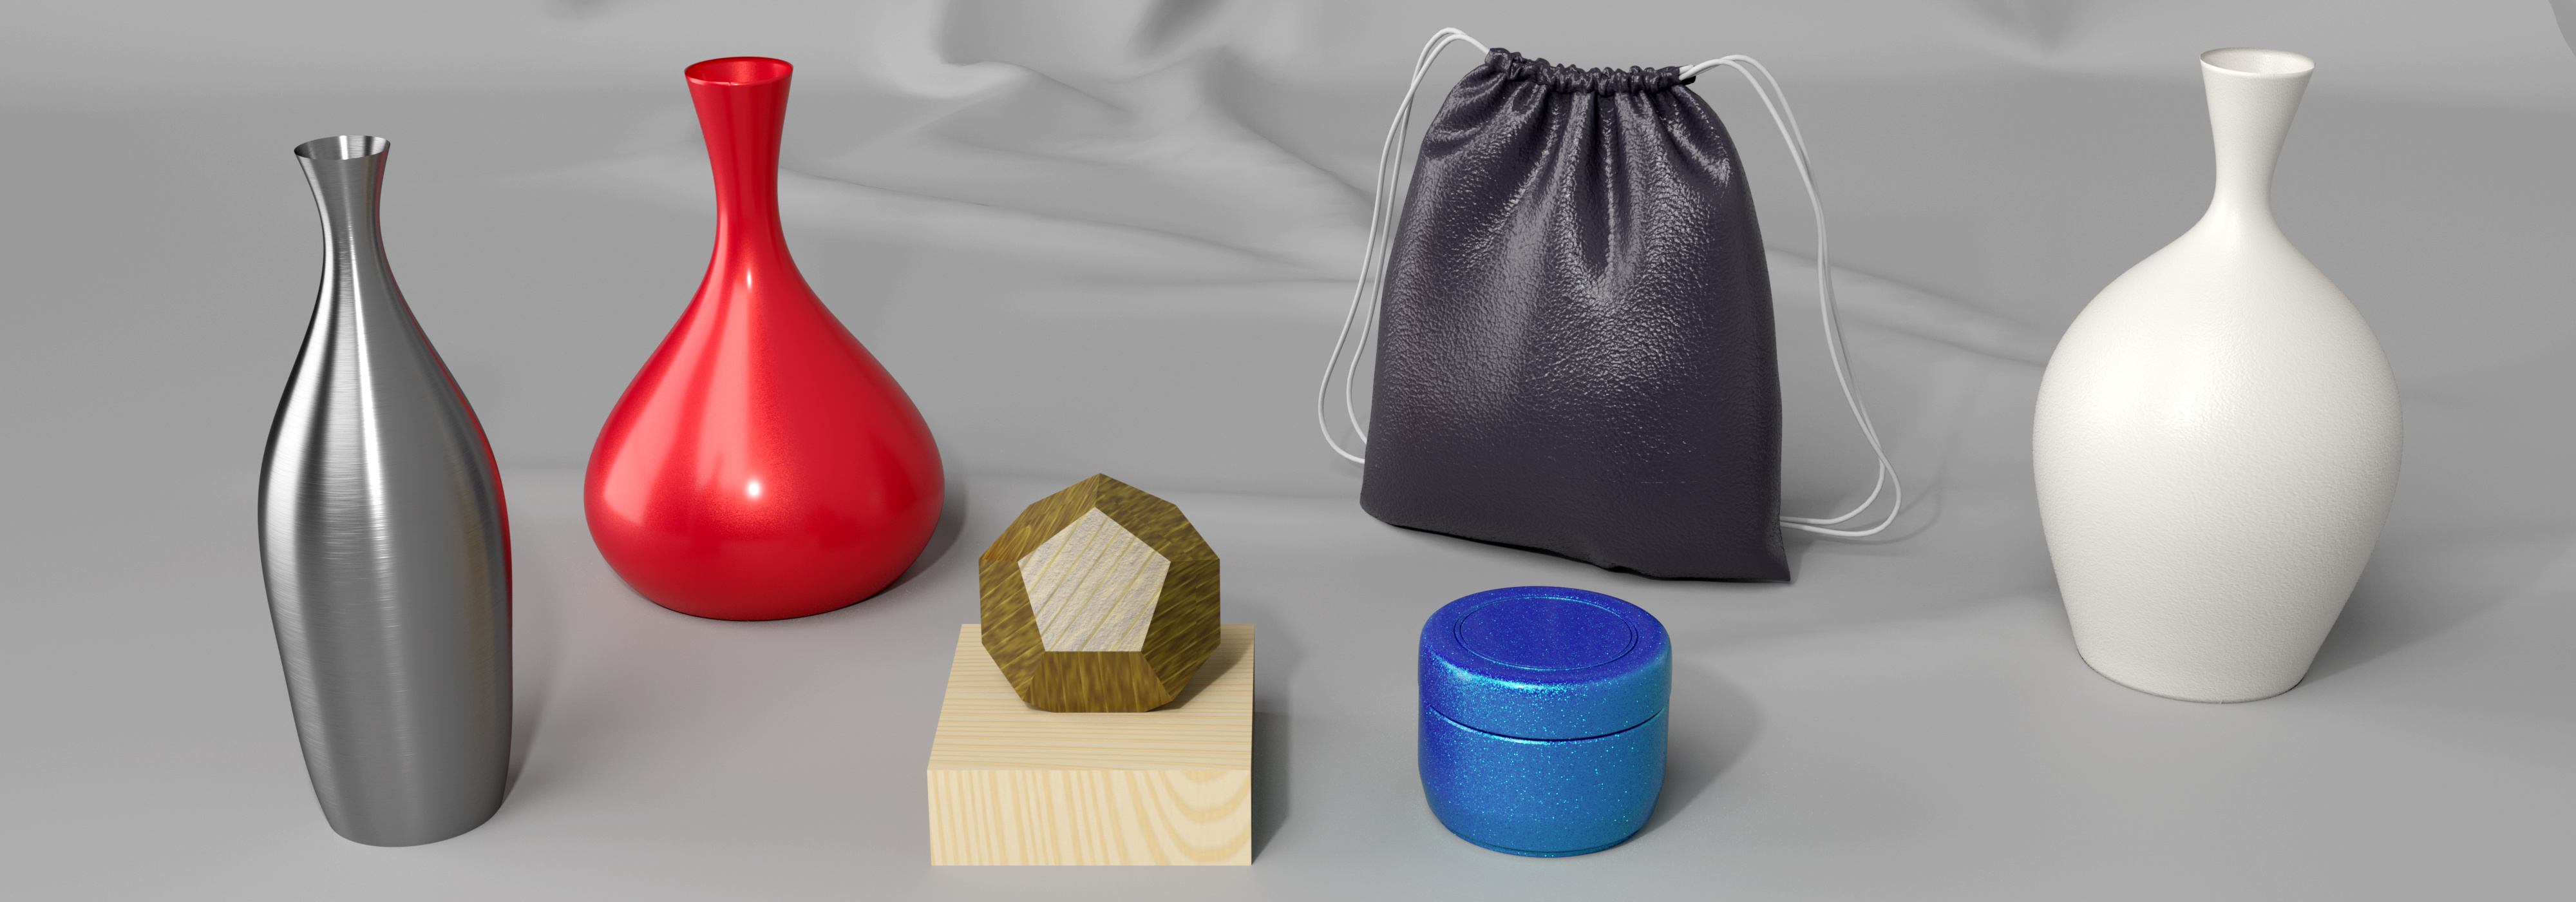
\includegraphics[width=\textwidth]{bayesian/fig1-2/teaser.jpg}\\[2pt]
	\begin{tabular}{cccccccc}
		\raisebox{\raiseLen}{\rotatebox{90}{Input}} &
		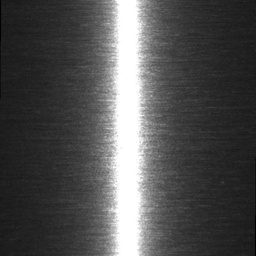
\includegraphics[width=\resLen]{bayesian/fig7/5_metal_3/target.jpg} &
		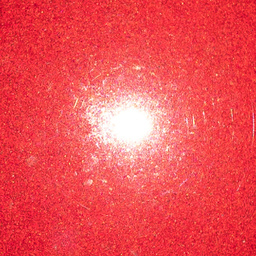
\includegraphics[width=\resLen]{bayesian/fig7/4_flake_4/target.jpg} &
		
\includegraphics[width=\resLen]{bayesian/fig7/6_wood_4/target.jpg} &
		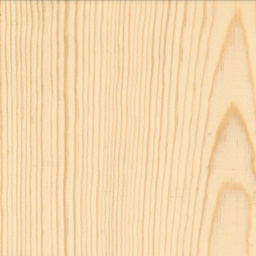
\includegraphics[width=\resLen]{bayesian/fig7/6_wood_5/target.jpg} &
		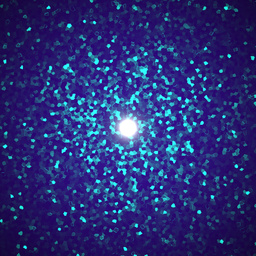
\includegraphics[width=\resLen]{bayesian/fig5/4_flake_1/target.jpg} &
		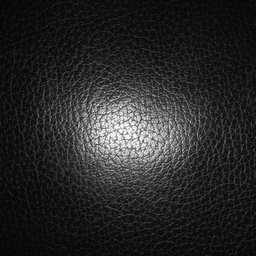
\includegraphics[width=\resLen]{bayesian/fig7/2_leather_3/target.jpg} &
		
\includegraphics[width=\resLen]{bayesian/fig7/1_bump_4/target.jpg}
		\\
		\raisebox{\raiseLen}{\rotatebox{90}{Rendered}} &
		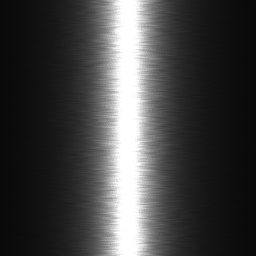
\includegraphics[width=\resLen]{bayesian/fig7/5_metal_3/good1.jpg} &
		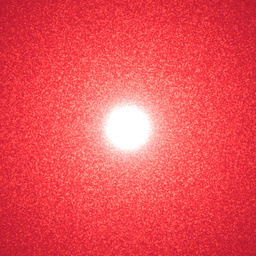
\includegraphics[width=\resLen]{bayesian/fig7/4_flake_4/good1.jpg} &
		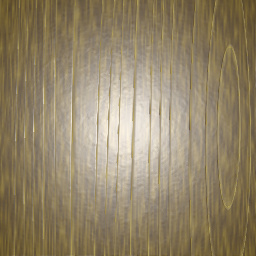
\includegraphics[width=\resLen]{bayesian/fig7/6_wood_4/good1.jpg} &
		
\includegraphics[width=\resLen]{bayesian/fig7/6_wood_5/good1.jpg} &
		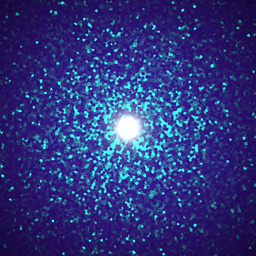
\includegraphics[width=\resLen]{bayesian/fig5/4_flake_1/good1.jpg} &
		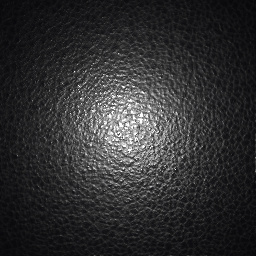
\includegraphics[width=\resLen]{bayesian/fig7/2_leather_3/good1.jpg} &
		
\includegraphics[width=\resLen]{bayesian/fig7/1_bump_4/good1.jpg}
	\end{tabular}
	\caption[Teaser]{\label{fig:bayesian:teaser}
		A scene rendered with material parameters estimated using our method: bumpy dielectrics, leather, plaster, wood, brushed metal, and metallic paint. The insets show a few examples of the input (target) images, and renderings produced using our procedural models with parameters found by Bayesian posterior sampling.
 	}
\end{figure}

\section{Introduction}
\label{sec:bayesian:intro}

Physically accurate simulation of material appearance is an important yet challenging problem, with applications in areas from entertainment to product design and architecture visualization.
A key ingredient to photorealistic rendering is high-quality material appearance data.
Acquiring such data from physical measurements such as photographs has been an active research topic in computer vision and graphics. Recently, \emph{procedural} material models have been gaining significant traction in the industry (e.g., Substance \cite{adobe2019substance}).
In contrast to traditional texture-based spatially varying BRDFs that represent the variation of surface albedo, roughness, and normal vectors as 2D images, procedural models generate such information using a smaller number of user-facing parameters, providing high compactness, easy editability, and automatic seamless tiling.

The estimation of procedural model parameters faces several challenges. First, the procedural generation and physics-based rendering of materials is a complex process with a diverse set of operations, making the relationship between procedural model parameters and properties of the final renderings non-linear and non-trivial.
Additionally, designing a suitable loss function (metric) to compare a synthesized image to a target image is not obvious. Finally, given the soft nature of the image matching problem, a single point estimate of the ``best'' match may be less informative than a collection of plausible matches that a user can choose from.

In this paper, we introduce a new computational framework to estimate the parameters of procedural material models that focuses on these issues.
Our framework enjoys high generality by not requiring the procedural model to take any specific form, and supporting any differentiable BRDF models, including anisotropy and layering.

To design the loss function, we consider neural summary functions (embeddings) based on Gram matrices of VGG feature maps \cite{gatys2015neural,gatys2016image}, as well as hand-crafted summary functions (\S\ref{sec:bayesian:summary}). The VGG feature map approach is becoming standard practice in computer vision, and was first introduced to material capture by Aittala et al. \cite{aittala2016reflectance}; we extend this approach to procedural material estimation.

We make two main contributions. The first contribution is a unified view of the procedural parameter estimation problem in a \emph{Bayesian framework} (\S\ref{sec:bayesian:param}), precisely defining the posterior distribution of the parameters given the captured data and priors, allowing for both maximization and sampling of the posterior. Four components (priors, procedural material model, rendering operator, summary function) together define our posterior distribution (outlined in Figure \ref{fig:bayesian:pipeline}). 

\input{tex/bayesian/fig/pipeline}

Our second contribution is to introduce a \emph{Bayesian inference} approach capable of drawing samples from the space of plausible material parameters.
This provides additional information beyond single point estimates of material parameters (for example, though not limited to, discovering similarity structures in the parameter space).
Further, due to an ability to combine multiple Markov-Chain Monte Carlo (MCMC) sampling techniques such as Metropolis-Hasting (MH), Hamiltonian Monte Carlo (HMC), and Metropolis-adjusted Langevin algorithm (MALA), our technique is capable of efficiently handling both discrete and continuous model parameters.
Posterior sampling is a well-studied area within statistics and has been used in computer vision and inverse rendering \cite{kulkarni2015picture}, but to our knowledge, it has not yet been applied to material appearance acquisition.

To demonstrate the effectiveness of our framework, we fit procedural models for a diverse set of materials from standard opaque dielectrics (e.g. plastics, leather, wall paint) to dielectrics with 3D structure (wood) to anisotropic brushed metals and layered metallic paints (see Figure~\ref{fig:bayesian:teaser}, \S\ref{sec:bayesian:results}, and the supplemental materials).


\section{Related Work}
\label{sec:prior_work}
%
We review previous work on material parameter estimation in computer graphics and vision, as well as on Markov-Chain Monte Carlo (MCMC) methods in Bayesian inference.

\paragraph*{SVBRDF capture.} A large amount of previous work focuses on acquisition of material data from physical measurements. The methods generally observe the material sample with a fixed camera position, and solve for the parameters of a spatially-varying BRDF model such as diffuse albedo, roughness (glossiness) and surface normal. They differ in the number of light patterns required and their type; the patterns used include moving linear light \cite{Gardner2003}, Gray code patterns \cite{Francken2009} and spherical harmonic illumination \cite{Ghosh2009}. In these approaches, the model and its optimization are specific to the light patterns and the optical setup of the method, as general non-linear optimization was historically deemed  inefficient and not robust enough.

More recently, Aittala et al. \cite{Aittala2013} captured per-pixel SVBRDF data using Fourier patterns projected using an LCD screen; their algorithm used a fairly general, differentiable forward evaluation model, which was inverted in a maximum a-posteriori (MAP) framework. Later work by Aittala et al. \cite{Aittala2015,Aittala2016} found per-pixel parameters of stationary spatially-varying SVBRDFs from two-shot and one-shot flash-lit photographs, respectively. In the latter case, the approach used a neural Gram-matrix texture descriptor based on the texture synthesis and feature transfer work of Gatys \cite{Gatys2015,Gatys2016} to compare renderings with similar texture patterns but without pixel alignment. We demonstrate that this descriptor makes an excellent summary function within our framework; in fact, the approach works well in our case, as the procedural nature of the model serves as an additional implicit prior, compared to per-pixel approaches. On the other hand, our forward evaluation process is more complex than Aittala et al., since it also includes the procedural material generation itself.

Recent methods by Deschaintre et al. \cite{Deschaintre2018}, Li et al. \cite{Li2018} have been able to capture non-stationary SVBRDFs from a single flash photograph by training an end-to-end deep convolutional network. Gao et al. \cite{Gao2019} introduced an auto-encoder approach, optimizing the appearance match in the latent space. All of these approaches estimate per-pixel parameters of the microfacet model (diffuse albedo, roughness, normal), and are not obviously applicable to estimation of procedural model parameters, nor to more advanced optical models (significant anisotropy, layering or scattering).

\paragraph*{Procedural material parameter estimation.} Focus on estimating the parameters of procedural models has been relatively rare. The dual-scale glossy parameter estimation work of Wang et al. \cite{Wang2011} finds, under step-edge lighting, the parameters of a bumpy surface model consisting of a heightfield constructed from a Gaussian noise power spectrum and global microfacet material parameters. Their results provide impressive accuracy, but the solution is highly specialized for this material model and illumination.

Recently, Hu et al. \cite{Hu2019} introduced a method for inverse procedural material modeling that treats the material as a black box, and trains a neural network mapping images to parameter vector predictions. The training data comes from evaluating the black box model for random parameters. In our experiments, this approach was less accurate; our fully differentiable models can achieve higher accuracy fits and can be used to explore posterior distributions through sampling. In a sense, this neural prediction method could be seen as orthogonal to ours, as we could use it for initialization of our parameter vector, continuing with our MCMC sampling.

\paragraph*{Optical parameters of fiber-based models.} Several approaches for rendering of fabrics model the material at the microscopic fiber level \cite{Zhao2011,Zhao2016,Leaf2018}. However, the optical properties of the fibers (e.g. roughness, scattering albedo) have to be chosen separately to match real examples. Zhao et al. \cite{Zhao2011} use a simple but effective trick of matching the mean and standard deviation (in RGB) of the pixels in a well-chosen area of the target and simulated image. Khungurn et al. \cite{Khungurn2015} have extended this approach with a differentiable volumetric renderer, combined with a stochastic gradient descent; however, their method is still specific to fiber-level modeling of cloth.

\paragraph*{Bayesian inference and MCMC.} A variety of methods used across the sciences are Bayesian in nature; in this paper, we specifically explore Bayesian inference for parameter estimation through Markov-Chain Monte Carlo (MCMC) sampling of the posterior distribution. Provided a nonnegative function~$f$, MCMC techniques can draw samples from the probability density proportional to the given function~$f$ without knowing the normalization factor. Metropolis-Hastings \cite{Hastings} is one of the most widely used MCMC sampling methods. If $f$ is differentiable, the presence of gradient information leads to more efficient sampling methods such as Hamiltonian Monte Carlo (HMC)~\cite{Neal2012,Betancourt2017} and Metropolis-adjusted Langevin algorithm (MALA)~\cite{MALA}.
Our inference framework is not limited to any specific MCMC sampling technique.
In practice, our implementation handles discrete model parameters using MH and continuous ones using MALA (with preconditioning~\cite{Santa}). We opt MALA for its simpler hyper-parameter tweaking (compared to HMC).

%Several software packages exist for Bayesian inference, allowing a user to specify a statistical forward model and parameters, handling the MCMC sampling; an example is STAN \cite{Stan}. Our earlier version was based on STAN. We reimplemented our system in PyTorch, which gave our system higher flexibility and extensibility.

\paragraph*{MCMC applications in graphics and vision.} Markov chain Monte Carlo techniques have been heavily studied in rendering, though not for Bayesian inference, but rather for sampling light transport paths with probability proportional to their importance; notably Metropolis light transport \cite{MLT} and its primary sample space variant \cite{Kelemen}. Much further work has built on these techniques, including more recent work that uses a variant of Hamiltonian Monte Carlo \cite{H2MC}. However, all of these approaches focus on better sampling for traditional rendering, rather than parameter estimation in inverse rendering tasks.

In computer vision, Bayesian inference with MCMC has been used for the inverse problems of scene understanding. A notable previous work is Picture \cite{Picture}, a probabilistic system and programming language for scene understanding tasks, for example (though not limited to) human face and body pose estimation. The programming language is essentially used to specify a forward model (e.g., render a face in a given pose), and the system then handles the MCMC sampling of the posterior distribution through a combination of sampling (proposal) techniques. This is closely related to the overall design of our system. However, the Picture system does not appear to be publicly available, and our application is fairly distant from its original goals.


\section{Preliminaries}
\label{sec:bayesian:prelim}

\paragraph{Procedural model generation.}
We focus on \emph{procedural material models} which utilize specialized procedures (pieces of code) to generate spatially varying surface reflectance information.
Specifically, let $\bmtheta$ be the parameters taken by some procedural material generation process $f_0$.
Then, $f_0(\bmtheta)$ generates the material properties (e.g., albedo, roughness, surface normals, anisotropy, scattering, etc.), in addition to any other parameters required by rendering (e.g. light parameters), which can in turn be converted into a synthetic image $\bmIs$ via a rendering operator $R$.
This \emph{forward evaluation} process can be summarized as
\begin{equation}
	\label{eq:forward}
	\bmIs = R(f_0(\bmtheta)) = f(\bmtheta),
\end{equation}
where $f$ is the composition of $R$ and $f_0$.
When modeling real-world materials, it is desirable to capture naturally arising irregularities.
In procedural modeling, this is usually achieved by making the model generation process $f_0$ to take extra random input $\bmz$ (e.g., random seeds, pre-generated noise textures, etc.) that is then used to create the irregularities.
This also causes the full forward evaluation to become $f(\bmtheta; \bmz) := R(f_0(\bmtheta; \bmz))$.

\paragraph{Continuous and discrete parameters.}
While most procedural material parameters tend to be continuous, discrete parameters can be useful for switching certain components on and off, or for choosing between several discrete noise types. We model this by splitting the parameter vector into continuous and discrete components, $\bmtheta = (\bmtheta_c, \bmtheta_d)$.
We assume the forward evaluator $f$ to be differentiable with respect to $\bmtheta_c$ (but not $\bmtheta_d$ or the random input $\bmz$).

\paragraph{Inverse problem specification.}
We consider the problem of inferring procedural model parameters $\bmtheta$ given a target image $\bmIt$  (which is typically a photograph of a material sample under known illumination).
This, essentially, requires inverting $f$ in Eq. \eqref{eq:forward}: $\bmtheta = f^{-1}(\bmIt)$. Direct inversion of $f = R \circ f_0$ is intractable for any but the simplest material and rendering models.
Instead, we aim to identify a collection of plausible values $\bmtheta$ such that $\bmIs$ has similar appearance to $\bmIt$:
\begin{equation}
	\label{eq:approx}
	\mbox{find examples of } \ \bmtheta \ \mbox{s.t.} \ \bmIt \approx f(\bmtheta; \bmz),
\end{equation}
for some (any) $\bmz$, where $\approx$ is an \emph{appearance-match} relation that will be discussed in the next section.

\section{Summary Functions}
\label{sec:bayesian:summary}

To solve the parameter estimation problem using Eq. \eqref{eq:approx}, a key ingredient is the appearance-match relation.
Unfortunately, we cannot use simplistic image difference metrics such as the L2 or L1 norms.
This is because the features (bumps, scratches, flakes, yarns, etc.) in the images of real-world materials are generally misaligned, even when the two images represent the same material.
In procedural modeling, as shown in Figure \ref{fig:bayesian:sum_func}, with irregularities created differently using $\bz_1$ and $\bz_2$, the same procedural model parameters $\btheta$ can yield slightly different results $f(\btheta; \bz_1)$ and $f(\btheta, \bz_2)$.

\input{tex/bayesian/fig/sum_func}

To overcome this challenge, we use the concept of a \emph{summary function}, which abstracts away the unimportant differences in the placement of the features, and summarizes the predicted and target images into smaller vectors whose similarity can be judged with simple metrics like L2 distance.
We define an image summary function $\summ$ to be a continuous function that maps an image of a material ($\target$ or $\synth$) into a vector in $\Reals^k$. An idealized summary function would have the property that
\begin{equation}
	\summ(f(\btheta_1, \bz_1)) = \summ(f(\btheta_2, \bz_2)) \ \Leftrightarrow \ \btheta_1 = \btheta_2.
\end{equation}
That is, applying the summary function would abstract away from the randomness $\bz$ and the difference between the two summary vectors would be entirely due to different material properties $\btheta$. Practical summary functions will satisfy the above only approximately. However, a good practical summary function will embed images of the same material close to each other, and images of different materials further away from each other. Below we discuss several techniques for constructing summary functions.

\paragraph{Neural summary function.}
Gatys et al. \cite{gatys2015neural,gatys2016image} introduced the idea of using the features of an image classification neural network (usually VGG \cite{simonyan2014very}) as a descriptor $T_G$ of image texture (or style). Optimizing images to minimize the difference in $T_G$ (combined with other constraints) allowed Gatys et al. to produce impressive, state-of-the art results for parametric texture synthesis and style transfer between images. While further work  has introduced improvements \cite{risser2017stable}, we find that the original version from Gatys et al. works already well in our case.

Aittala et al. \cite{aittala2016reflectance} introduced this technique to capturing material parameter textures (albedo, roughness, normal and specular maps) of stationary materials. They optimized for a $256 \times 256$ stationary patch that matches the target image in various crops, using a combination of $T_G$ and a number of special Fourier-domain priors. In our case (for procedural materials), we find that the neural summary function $T_G$ works even more effectively; we can simply apply it to the entire target or simulated images (not requiring crops nor Fourier-domain priors).

Specifically, define the Gram matrix $G$ of a set of feature maps $F_1, \cdots, F_n$ such that it has elements
\begin{equation}
	G_{ij} = \mbox{mean}(F_i \cdot F_j),
\end{equation}
where the product $F_i \cdot F_j$ is element-wise. $T_G$ is defined as the concatenation of the flattened Gram matrices computed for the feature maps before each pooling operation in VGG19. Note that the size of the Gram matrices depends on the number of feature maps (channels), not their size; thus $T_G$ is independent of input image size.

\paragraph{Statistics and Fourier transforms of image bins.}
While the neural summary function performs quite well, we find that in some cases we can improve upon it.
A simple idea for a summary function is to use the (RGB) mean of the entire image; an improvement is to subdivide the image into $k$ bins (regions) and compute the mean of each region. We found concentric bins perform well for isotropic materials, and vertical bins are appropriate for anisotropic highlights (e.g. brushed metal). Furthermore, we can additionally use a fast Fourier transform of the entire image or within bins. Note that automatic computation of derivatives is possible with the FFT, and supported by the PyTorch framework. In our current results, we use a summary function that combines the means and 1D FFTs of 64 vertical bins for the brushed metal example; all other examples use the neural summary function combined with simple image mean.

\section{Bayesian Inference of Material Parameters}
\label{sec:bayesian:param}

In what follows, we first describe a Bayesian formulation of the estimation problem in terms of a posterior distribution. Next, we discuss how to use the posterior for point estimation in a maximum a-posteriori (MAP) framework, and how the Markov-Chain Monte Carlo (MCMC) methods for Bayesian inference extend the point estimate approach by sampling from the posterior.


\subsection{Bayesian formulation}
\label{ssec:point_sec}

We treat the procedural model parameters $\bmtheta$ as random variables with corresponding probability distributions.

We first introduce a \emph{prior} probability distribution $p(\bmtheta)$ of the parameters, reflecting our pre-existing beliefs about the likelihood values of the unknown parameters. For example, for most material categories, we know what range the albedo color and roughness coefficients of the material should typically be in.

Further, we model the $\approx$ operator from Eq. \eqref{eq:approx} as an error distribution. Specifically, we postulate that the difference between the simulated image summary $\calS(f(\bmtheta, \bmz))$ and the target image summary $\calS(\bmIt)$ follows a known probability distribution.
In practice, we use a (multi-variate) normal distribution with zero mean and the covariance $\bmSigma_e$:
\begin{equation}
	\calS(f(\bmtheta, \bmz)) - \calS(\bmIt) \sim \mathcal{N}(0, \bmSigma_e).
\end{equation}
Our experiments indicate that this simple error distribution works well in practice, and we regard $\bmSigma_e$ as a hyper-parameter and set it manually.

We also have multiple options in handling the random vector $\bmz$. While it is certainly theoretically possible to estimate it, we are not really interested in its values;  we find it simpler and more efficient to simply choose $\bmz$ randomly, fix it, and assume it known during the process of estimating the ``interesting'' parameters $\bmtheta$.
Under these assumptions, according to the Bayes theorem, we can write down the posterior probability of parameters $\bmtheta$, conditional on the known values of $\bmIt$ and $\bmz$, as:
\begin{equation} 
	\label{eq:posterior}
	p(\bmtheta | \bmIt, \bmz) \propto \mathcal{N}\left[\calS(f(\bmtheta, \bmz)) - \calS(\bmIt); 0, \bmSigma_e\right] p(\bmtheta),
\end{equation}
where the right side does not need to be normalized; the constant factor has no effect on parameter estimates.
For numerical stability, we compute the negative log posterior, viz. $-\log p(\bmtheta | \bmIt, \bmz)$, in practice. Equation~\eqref{eq:posterior} also holds when $\bmtheta$ involves discrete parameters, as long as the prior is properly defined as a product of a continuous pdf $p(\bmtheta_c)$ and a discrete probability $p(\bmtheta_d)$.

\subsection{Point estimate of parameter values}

A point estimate of the parameter vector can be modeled in the maximum a-posteriori (MAP) framework. We simply estimate the desired parameter values $\bmtheta$ as the maximum of the posterior pdf $p(\bmtheta | \bmIt, \bmz)$ given by Eq. \eqref{eq:posterior}. For continuous $\bmtheta$, this problem can be solved using standard non-linear optimization algorithms. In the presence of discrete parameters, there is no single accepted solution. While various heuristics could be used, our sampling approach described below provides a cleaner solution to discrete parameter estimation.

\subsection{Markov-Chain Monte Carlo Sampling of the Posterior}
\label{ssec:bayesian}

Although the point estimate approach gives satisfactory results in many cases, it is not without problems. For example, since a perfect match between a procedural material and a photograph is generally impossible, it can be desirable to have a set of imperfect matches for the user to choose from. Further, there could be an entire subset of the parameter space giving solutions of approximately equivalent fit under the target view and lighting; however, these may look quite different from each other in other configurations, and a user may want to explore those differences. Lastly, with the presence of discrete parameters, it is not obvious how to solve the maximization in Eq. \eqref{eq:posterior} efficiently.

In this chapter, we use the well-known technique of full Bayesian inference, sampling the posterior pdf defined in Eq.~\eqref{eq:posterior} using Markov-Chain Monte Carlo (MCMC) techniques, specifically Metropolis-Hasting (MH)~\cite{hastings1970monte}, Hamiltonian Monte Carlo (HMC) \cite{betancourt2017conceptual}, and Metropolis-adjusted Langevin algorithm (MALA)~\cite{roberts1996exponential}. While well explored in statistics and various scientific fields, to our knowledge, this technique has not been used for the inference of material parameters.

The goal of the sampling is to explore the posterior with many (typically thousands or more) samples, each of which represents a material parameter vector consistent with the target image. Plotting these samples projected into two dimensions (for a given pair of parameters) gives valuable insight into similarity structures. Furthermore, interactively clicking on samples and observing the predicted result can help a user to quickly zoom in on a preferred solution, which an automatic optimization algorithm is fundamentally incapable of.

\input{tex/bayesian/alg/sample}

Algorithm \ref{alg:bayesian:sample} summarizes our MCMC sampling process. At each iteration, we mutate either the continuous parameters (with probability $\alpha$) or the discrete ones (with probability $1 - \alpha$).
For the former case, we utilize the gradient of the log pdf with respect to $\bmtheta_c$ to efficiently obtain a new proposal $\bmtheta_c'$ (Line \ref{alg:line:malaSample}).
Our implementation uses MALA for this process, although HMC could also work.
For the latter case, we obtain a new proposal $\bmtheta_d'$ of the discrete parameters, currently by uniformly sampling their joint probability mass function (Line \ref{alg:line:mhSample}).
Upon obtaining a full proposal, we use the standard Metropolis-Hasting rule (Line \ref{alg:line:mhAccRej}) to stochastically select the new sample $(\bmtheta_c^{(t + 1)}, \bmtheta_d^{(t + 1)})$ by either accepting the newly proposed $(\bmtheta_c', \bmtheta_d')$ or (rejecting the proposal and) keeping the previous sample $(\bmtheta_c^{(t)}, \bmtheta_d^{(t)})$.

\section{Material Models and Results}
\label{sec:bayesian:results}

\textbf{(Only a small subset of our results fits into the thesis. Please see our supplemental material and video for more results.
[\href{https://www.ics.uci.edu/~yug10/webpage/suppl/2020CGF/index.html}{Click here}])}


We now demonstrate the effectiveness of our technique by fitting several procedural material models to a mix of synthetic and real target images.

Our forward evaluation process uses collocated camera and light.
This configuration closely matches a mobile phone camera with flash (which is used for most of the real target images) and simplifies some BRDF formulations (because the incoming, outgoing, and half-way vectors are all identical).
Further, we assume that the distance between camera and sample is known as it is generally easy to measure or estimate.
The knowledge of the camera field of view allows us to compute the physical scale of the resulting pixels.
Lastly, we treat light intensity and camera vignetting (expressed as an image-space Gaussian function) as (unknown) parameters of the forward evaluation process so that they do not need to be calibrated.
Our parameter inference framework presented in \S\ref{sec:bayesian:summary} and \S\ref{sec:bayesian:param} is not limited to this specific setup.

All the procedural material models we used, which will be detailed in \S\ref{ssec:proc_models}, are implemented using \textsf{PyTorch} which automatically provides GPU acceleration and computes derivatives through backpropagation. 
For all material parameter inference tasks, our forward evaluation generates $512 \times 512$ images.
Notice that the recovered parameters can then be used to generate results with much higher resolution because the procedural models are generally resolution-independent.

\subsection{Similarity Relations in Translucency}

As a motivating example, we first illustrate the behavior of the MCMC material parameter estimation process on the case of a homogeneous translucent material with two varying parameters.
In this example, the shape of the posterior can be analytically derived (using the similarity theory) and easily plotted. This serves as a demonstration and validation of our approach.

\input{tex/bayesian/fig/scatter}

Specifically, the material parameter space of translucent materials under the radiative transfer framework \cite{chandrasekhar1960radiative} is known to be approximately over-complete~\cite{zhao2014high}.
Specifically, two sets of parameters $(\sigma_s, \sigma_a, g)$ and $(\sigma_s^*, \sigma_a^*, g^*)$ satisfying the following \emph{similarity relation} usually yield similar final appearances:
\begin{equation}
	\label{eq:similarity_rel}
	\sigma_a = \sigma_a^*, \quad (1 - g)\,\sigma_s = (1 - g^*)\,\sigma_s^*,
\end{equation}
where $\sigma_a$ and $\sigma_s$ are, respectively, the absorption and scattering coefficients, and $g$ is the first Legendre moment of the phase function.
We show in Figure~\ref{fig:bayesian:scatter} that applying our Bayesian inference method to $\sigma_s$ and $g$ (with fixed $\sigma_a$) computes a posterior distribution that agrees well with the predicted similarity relation~\eqref{eq:similarity_rel}.


\subsection{Procedural Material Models}
\label{ssec:proc_models}

We show results generated using synthetic images in Figures \ref{fig:bayesian:synthetic} and \ref{fig:bayesian:discrete} as well as real photographs (taken with different cameras) in Figure \ref{fig:bayesian:real}.
Please see the supplemental material for more results, including animations illustrating point estimations and sampling. Below we describe the six procedural models tested. Please refer to the supplement for additional detail and a \textsf{PyTorch} implementation. For each parameter, we define a reasonable truncated Gaussian distribution as its prior (also see supplement). In most cases, the MCMC sampling starts from the peak of the prior. In some examples (e.g wood), we first run posterior maximization and then switch to sampling from the optimized point. We drop some number (typically 200 to 1000) of initial MCMC samples due to burn-in.

\input{tex/bayesian/tab/performance}

\input{tex/bayesian/fig/synthetic}

\input{tex/bayesian/fig/discrete}

\input{tex/bayesian/fig/real}

\paragraph{Bumpy microfacet surface.}
This model depicts an opaque dielectric surface with an isotropic noise heightfield. We use a standard microfacet BRDF with the GGX normal distribution \cite{walter2007microfacet} combined with a normal map computed from an explicitly constructed heightfield. We assume that the Fresnel reflectance at normal incidence can be computed from a known index of refraction (a value of 1.5 is a good estimate for plastics). We assume an unknown roughness $r$ (GGX parameter $\alpha=r^2$) and a Lambertian diffuse term with unknown albedo $\rho$. This model is identical to Wang et al. \cite{wang2011estimating}, except using the GGX instead of Beckmann microfacet distribution. The main practical difference from the capture setup in that paper is that we use a point light, instead of step-edge illumination.

The bumpy heightfield is constructed using an inverse Fourier process including: (i) choosing a power spectrum in the continuous Fourier domain; (ii) discretizing it onto a grid of complex numbers; (iii) randomly choosing the phase of each texel on the grid (while keeping the chosen amplitude); and (iv) applying an inverse fast Fourier transform whose
real component becomes the resulting heightfield.
At render time, we use the normal map derived from this heightfield.

\paragraph{Leather and plaster.}
These materials can be modeled similarly as the aforementioned bumpy surfaces except for the computation of the heightfield and roughness.
For plaster, a fractal noise texture is scaled (in space and intensity) and thresholded (controlled by additional parameters) to produce both the heightfield and a roughness variation texture. For leather, on the contrary, a Voronoi cell map is used to get the effect of leather-like cells (with parameters for scaling and thresholding), and additional small-scale fractal noise is added.
Further, we use multiple (pre-generated) noise textures and Voronoi cell maps to diversify the micro-scale appearances that our models can produce.
The choice of these textures and maps is captured using a discrete parameter.
In Figure~\ref{fig:bayesian:discrete}, we show a few example samples drawn from the posterior distributions using Algorithm~\ref{alg:bayesian:sample}.

\paragraph{Brushed metal.} The brushed metal material extends the above bumpy surface, by introducing anisotropy to both the GGX normal distribution and the noise heightfield used to compute the normal map, while dropping the diffuse term. We make both the BRDF and the Fourier-domain Gaussian power spectrum anisotropic. The parameters of the model thus include two roughnesses, as well as two Fourier-domain standard deviations.  We make the anisotropic highlight vertical and centered in the target image.

\paragraph{Metallic flakes.} Metallic paint with flakes is a stochastic material with multiple BRDF lobes (caused by light reflecting off the flakes). Our model involves three components, each being an isotropic microfacet lobe, to describe top coating, flakes and glow, respectively. The top coating is usually highly specular, and we make its roughness a model parameter. We assume an index of refraction of 1.5, implying a Fresnel (Schlick) reflectivity at normal incidence of 0.04. The flakes are chosen as Voronoi cells of a random blue-noise point distribution; they have a roughness parameter and varying normals chosen from the Beckmann distribution with an unknown roughness, and with unknown Fresnel reflectivity. The scale of the cell map is itself a (differentiable) parameter. Lastly, the glow is a component approximating the internal scattering between the top interface and the flakes, and has its own roughness, Fresnel reflectivity and a flat normal. An extra weight parameter linearly combines the flakes and the glow.

\paragraph{Wood.} We also created a partial \textsf{PyTorch} implementation of the comprehensive 3D wood model of Liu et al.~\cite{liu2016simulating}. This material is a 3D model of the growth rings of a tree, with a number of parameters controlling colors and widths of growth rings, as well as global distortions and small-scale noise features. The 3D wood is finally projected by a cutting plane to image space, defining diffuse albedo, roughness and height.


\input{tex/bayesian/fig/mismatch}

\paragraph{Mismatched models.}
Lastly, we demonstrate in Figure \ref{fig:bayesian:mismatch} the impact of forward procedural models.
Since these model-generating procedures are essentially material-specific priors, using mismatched models generally leads to results that match overall image statistics but with incorrect patterns.

\subsection{Additional Comparisons}

\input{tex/bayesian/fig/aittala}

\paragraph{Comparison to Aittala et al.}
We first compare our technique to with one introduced by Aittala~et~al. \cite{aittala2016reflectance} in Figure \ref{fig:bayesian:aittala} using input photos published as supplemental materials from their work.
Their work uses the same VGG-based loss (summary function), but optimizes directly in texture space. Both methods manage to reproduce the overall pattern and reflectance of the input photos.
Thanks to the underlying procedural models, our method is able to synthesize larger results without visually obvious periodic patterns, and with more plausible global variation.

\input{tex/bayesian/fig/hu}

\paragraph{Comparison to neural methods.}
We also compare our method with the forward neural prediction method of Hu et al. \cite{hu2019novel}. Their method uses an AlexNet network structure \cite{krizhevsky2012imagenet}, mapping an image of a material sample to the parameters of an appropriate procedural model. We apply their network structure with our BRDFs and lighting conditions, as their original implementation assumes Lambertian materials and outdoor sun/sky lighting. We show the results in Figure \ref{fig:bayesian:hu}. In general, we find the method gives moderately accurate results, which moreover tends to become worse for more complex BRDF models and with more parameters. The photo (top) is better matched by our MCMC sampling results (middle) than their prediction (bottom),

\input{tex/bayesian/fig/hu2}

To some extent, the method of \cite{hu2019novel} is orthogonal to ours, as it can be used as an efficient initialization for our sampling. In Figure \ref{fig:bayesian:hu2}, we compare our MCMC sampling results with a random starting point to one using the result of Hu et al. for initialization. This reduces the burn-in period required by the MCMC method.

\input{tex/bayesian/fig/des}

Finally, we also compare to the single input SVBRDF estimation method of Deschaintre et al. \cite{deschaintre2018single} (See Figure \ref{fig:bayesian:des}). This method takes a $256 \times 256$ target image, and produces material maps at the same resolution, pixel-wise aligned to the input. This pixel-wise alignment is not achievable with our method (or any procedural material estimation method). However, the overall perceptual appearance match is usually worse than our method. In some cases, the method produces specular burn-in, as the strong highlight cannot be fully removed and causes holes in the resulting maps (Plaster-4, Metallicflake-4). Advanced BRDF models like brushed metal and metallic flakes are not explicitly handled by their method and usually fail. Finally, their result is fixed at the $256 \times 256$ resolution, and does not support higher resolutions, seamless tiling, nor editability; these benefits come from the use of a procedural model.

Figure~\ref{fig:bayesian:plot} shows a quantitative comparison of the Learned Perceptual Image Patch Similarity (LPIPS) metric \cite{zhang2018unreasonable} between the captured photos and the re-renderings using different methods.

\input{tex/bayesian/fig/plot}

\section{Conclusion}
\label{sec:bayesian:conclusion}

Procedural material models have become increasingly more popular in the industry, thanks to their flexibility, compactness, as well as easy editability.
In this chapter, we introduced a new computational framework to solve the inverse problem: the inference of procedural model parameters based on a single input image.

The first major ingredient to our solution is a \emph{Bayesian framework}, precisely defining the posterior distribution of the parameters, combining four components (priors, procedural material model, rendering operator, summary function). The second ingredient is an \emph{Bayesian inference approach} that leverages MCMC sampling to sample posterior distributions of procedural material parameters.  This technique enjoys the generality to handle both continuous and discrete model parameters and provides users additional information beyond single point estimates and allows a cleaner extension to handle discrete parameters.

\chapter{Conclusion and Future work}
\label{cpt:conclusion}

In the dissertation, we focus on material appearances modeling in both forward and inverse rendering. All the macro appearances are modeled from microscales or hyperparameter spaces. 

First we have presented two scattering frameworks in forward rendering, one for layered materials (\emph{thin planer surface}) and the other one for participating medium (\emph{bulk,particles}). The first work \textbf{LayeredBSDF} provides a general solution to layered materials which is included in \emph{Physically Based Rendering}, Fourth Edition \cite{pharr2021physically}. It leads to the first BSDF layering solution that offers unbiased accuracy and full flexibility in setting the layer properties.
Our second work \textbf{Beyond Mie Theory} generalizes the widely-used Lorenz-Mie theory for rigorously deriving optical properties of scattering media, and can be readily used in any radiative-based light transport simulator.

Then we have estimated material properties using \emph{latent space} and \emph{procedural parameters}. Our third work \textbf{MaterialGAN} is the first step toward GAN-based material analysis and synthesis and our experiments suggest many avenues for further exploration. Our last work \textbf{Bayesian Inference Sampling} handles both continuous and discrete model parameters and provides users additional information beyond single point estimates and allows a
cleaner extension to handle discrete parameters.

At the end, we will discuss the limitation of our work and future directions:

\paragraph{LayeredBSDF}
Our model relies on the assumption of thin flat layers (Figure \ref{fig:layeredbsdf:zhaoyun}) and cannot capture effects caused by geometric or optical variations at the global scale.
Examples include internal caustics and shadowing arising from major normal variations and color bleeding caused by light scattering though media with varying colors.
Generalizing our technique to include bidirectional subsurface scattering distribution functions (BSSRDFs) is an interesting further topic.
In addition, as our model simulates subsurface scattering using Monte Carlo path tracing, the performance may degrade with the presence of optically thick layers with many scattering events.
Using fast approximated solutions such as \cite{jensen2001practical,frisvad2014directional} to capture multiple scattering may be a useful extension.
Lastly, since we model light transport using traditional radiative transfer, wave effects such as thin film interference are not handled.
An interesting challenge is to integrate wave optics into our model to accurately and efficiently handle light interference and phase shifts.

\paragraph{Beyond Mie Theory}
While taking into account the effect of the near-field on clusters, our work is still based on the RTT. Therefore it relies on the far-field approximation to represent a scattering dyad useful for rendering. Therefore, while we can handle near- and far-field scattering, we cannot accurately model the scattering in the intermediate region, which we treat as the far field. Using more accurate representations, that capture the effects at such near-field region could further enhance the generality of our theory and, thus, is an interesting future topic. This would however require exploring an alternative light transport framework beyond the RTT.
Right now, our implementation requires precomputing the bulk optical properties of the media. This limits the applicability of our work to media with homogeneous particle statistical properties. Finding faster approximations for our scattering functions, in the same spirit as the geometric optics approximation for Lorenz-Mie theory \cite{glantschnig1981light}, is an interesting future research. 
Finally, our implementation is currently limited in practice to spherical particles with identical radii within a particle cluster. Allowing general and spatially varying particle shapes by using an alternative implementation of the T-matrix method would further improve the versatility of our technique.

\paragraph{MaterialGAN}
Our current BRDF model is shared by previous work, but certain common effects (layering on book covers, subsurface fiber scattering in woods, anisotropy in fabrics) are not correctly captured by it. An extension of our generative model and rendering operator would be possible, though the key challenge is finding high-quality  training data for these effects.
Our assumption of almost flat samples will fail for materials with strong relief patterns, and will produce blurring or ghosting if there are obvious parallax effects in the aligned captured images. Strong self-shadowing or inter-reflections are also not currently handled. Solving for height instead of normal, with a more advanced rendering operator, may be able to resolve parallax effects and to correctly predict (and undo) shadowing effects from strong height variations.
Furthermore, more precise calibration may improve our accuracy. This would likely require knowledge of the cell phone hardware, and/or pre-calibration of its properties (e.g. flash light falloff, lens vignetting, and color processing properties).
The resolution of our result can be increased with a coarse-to-fine post-process, since we have a fairly good result as the initialization of next level of resolution.

\paragraph{Bayesian Inference Sampling}
In the future, we would like to increase the complexity of the models supported even further, to handle materials like woven fabrics, transmissive BTDFs, and more. Finally, extensions to our approach could be used to estimate parameters of procedural models beyond materials, including geometry and lighting, as long as the parameters could be differentiated.


% ... and so on

% These commands fix an odd problem in which the bibliography line
% of the Table of Contents shows the wrong page number.
\clearpage
\phantomsection

% "References should be formatted in style most common in discipline",
% abbrv is only a suggestion.
\bibliographystyle{plain}
\bibliography{references}

% The Thesis Manual says not to include appendix figures and tables in
% the List of Figures and Tables, respectively, so these commands from
% the caption package turn it off from this point onwards. If needed,
% it can be re-enabled later (using list=yes argument).
\captionsetup[figure]{list=no}
\captionsetup[table]{list=no}

% If you have an appendix, it should come after the references.
\begin{appendices}
% The original template (from Trevor) had a custom \appendix command,
% but I found it to break figure/table counters. I'm not sure how
% reliable my fix is, so I ended up reverting back to the standard
% latex version, and renaming the custom command to \myappendix.  You
% can try both and see how things work out:
% 1) Call \appendix once, and then make each appendix a \chapter
% 2) Call \myappendix once, and then make each appendix a \section.

\appendix
\chapter{Appendix for Chapter \ref{cpt:layeredbsdf}}
\section{Detailed Derivations}
\label{sec:derivation}

We now provide detailed derivations for the key equations in \S\ref{sec:path-formulation}.

\paragraph{Position-free radiative transfer equation.}
Traditionally, the radiative transfer equation (RTE) involves an integral over free-flight distance $t$:

%\begin{multline}
%\label{eq:IRTE0}
%  L_v(z, \bom) = S(z, \bom) \ + \\
%  \int_0^{t'} \exp(-t \sigma_t) \, \int_{\Sph} \hat f_p(\bom', \bom) \, L_v(z', \bom') \,\intd \bom' \intd t,
%\end{multline}
%
%where $z' := z - t\cos\bom$ and $t'$ denotes the distance between $z$ and the closest layer boundary.
%Since $t = (z - z')/\cos\bom$, changing the integration variable from $t$ to $z'$ in Eq.~\eqref{eq:IRTE0} yields an additional factor of $(\cos\bom)^{-1}$ which in turn gives our position-free RTE~\eqref{eq:IRTE}.
%Notice that the change-of-variable ratio only appears within the integration (and not in the source term $S$).
%
%\paragraph{Cosines in path contribution.}
%The contribution $f$ of a light path $\bar{x}$ can be obtained by repeatedly expanding the rendering equation~\eqref{eq:RE} and our position-free RTE~\eqref{eq:IRTE}.
%
%Similar to the traditional path integral formulation, for each vertex $z_i$ corresponding to an interface event (i.e., reflection or refraction), a cosine term $|\cos\bd_i|$ is needed to ensure the measure of projected solid angle.
%%For the volumetric scattering events, the cosine terms are absent (as the inner integral of the RTE~\eqref{eq:IRTE} already uses the solid angle measure).
%On the other hand, a segment of our light path connecting two depths $z_i$ and $z_{i + 1}$ via direction $\bd_i$ can yield an additional $|\cos\bd_i|^{-1}$ when $z_{i + 1}$ corresponds to a volumetric scattering.
%Thus, for each $i$, the path contribution involve a factor of $|\cos\bd_i|^{\alpha_i}$ with:
%%
%\begin{itemize}
%	\item $\alpha_i = 1$ if $z_i$ and $z_{i + 1}$ are both on interfaces;
%	\item $\alpha_i = 0$ (i.e., no $\cos\bd_i$ term) if (i)~$z_i$ is volumetric and $z_{i + 1}$ lies on an interface (so that no $\cos\bd_i$ terms appear during expansion), or (ii)~$z_i$ is interfacial and $z_{i + 1}$ is volumetric (so that both $|\cos\bd_i|$ and $|\cos\bd_i|^{-1}$ are present, canceling out each other);
%	\item $\alpha_i = -1$ if $z_i$ and $z_{i + 1}$ are both volumetric vertices.
%\end{itemize}
%%
%Eq.~\eqref{eqn:seg_contrib_cosine} provides a compact way to encode these rules. 

\section{Efficient Weight Computation}
\label{sec:layeredbsdf:weight_computation}


\paragraph{Weights of Light Transport Paths.}

Given a light subpath $\bar{x}_i$ and a camera subpath $\bar{x}_o$ with $n_i$ and $n_o$ vertices respectively, our bidirectional estimator combines $2 n_i n_o$ estimators of the form $f(\bar{y}^{(u)}_{s,t})/p^{(u)}_{s,t}(\bar{y}^{(u)}_{s,t})$ with $s \in \{1, 2, \ldots, n_i\}$, $t \in \{1, 2, \ldots, n_o\}$, and $u \in \{0, 1\}$ via the multiple importance sampling (MIS) framework.
This yields a combined estimator:
\begin{equation}
\label{eqn:bdpt_estimator}
\sum_{s = 1}^{n_i} \sum_{t = 1}^{n_o} \sum_{u = 0}^1 w^{(u)}_{s, t}(\bar{y}^{(u)}_{s,t}) \frac{f(\bar{y}^{(u)}_{s,t})}{p^{(u)}_{s,t}(\bar{y}^{(u)}_{s,t})},
\end{equation}
where the weight $w^{(u)}_{s, t}$, when using the balanced heuristics~[Veach 1997], is given by
\begin{equation}
\label{eqn:bdpt_weight_0}
w^{(u)}_{s, t}(\bar{y}_{s,t})
= \left(\sum_{s' = 1}^{s + t - 1} \sum_{u'=0}^1 \frac{p^{(u')}_{s', s + t - s'}(\bar{y}_{s,t})}{p^{(u)}_{s,t}(\bar{y}_{s,t})}\right)^{-1}
\end{equation}
for any path $\bar{y}_{s,t}$ with $(s + t)$ vertices.

Notice that, compared to standard bidirectional path tracing that combines $n_i n_o$ estimators, our position-free formulation offers twice the number of estimators since the direction connecting two depths is not unique.


\paragraph{Efficient Weight Computation.}

Computing Eqs. \eqref{eqn:bdpt_estimator} and \eqref{eqn:bdpt_weight_0} for all $s$ and $t$ na\"ively has a time complexity of $O(n_i n_o (n_i + n_o))$ and is too slow to be practical.
We now present our method that runs in $O(n_i n_o)$ time.
Our approach is conceptually similar to Veach's method for standard BDPT but differs in the exact mathematical form due to our position-free path formulation (see \S\ref{sec:layeredbsdf:ours}).

Let $\bar{y}_{s,t} = (\bd_0, z_1, \bd_1, \ldots, z_n, \bd_n)$ with $n = s + t$.
For all $s', t' \in \{ 1, 2, \ldots, n \}$, define
\begin{align}
p^{(0)}_{s'} &:= \prod_{i = 1}^{s' - 1} p( \bd_i \;|\; z_i, \bd_{i - 1} ) \, p( z_{i + 1} \;|\; z_i, \bd_i ),\\
p^{(1)}_{t'} &:= \prod_{i = n - t' + 1}^{n - 1} p( -\bd_i \;|\; z_{i + 1}, -\bd_{i + 1} ) \, p( z_i \;|\; z_{i + 1}, -\bd_i ),
\end{align}
which denote the probability for constructing two subpaths containing the first $s'$ and last $t'$ vertices of $\bar{y}$, respectively.
Then, for all $u'$, $s'$ and $t'$, it holds that
\begin{equation}
p^{(u')}_{s',t'}(\bar{y}_{s,t}) = p^{(0)}_{s'} \, p^{(1)}_{t'} \, q^{(u')}_{s'},
\end{equation}
where
\begin{equation}
q^{(u')}_{s'} := \begin{cases}
p( \bd_{s'} \;|\; z_{s'}, \bd_{s' - 1} ) & \text{if $u = 0$,}\\
p( -\bd_{s'} \;|\; z_{s' + 1}, -\bd_{s' + 1} ) & \text{if $u = 1$.}
\end{cases}
\end{equation}
It follows that
\begin{equation}
\label{eqn:bdpt_pdf_ratio_0}
\frac{p^{(u')}_{s', t'}(\bar{y}_{s,t})}{p^{(u)}_{s,t}(\bar{y}_{s,t})}
= \frac{p^{(0)}_{s'} \, p^{(1)}_{t'} \, q^{(u')}_{s'}}{p^{(0)}_s \, p^{(1)}_t \, q^{(u)}_s}.
\end{equation}
Note that, for any $s' < s$, we have
\begin{equation}
p^{(u')}_{s', t'}(\bar{y}_{s,t}) = p^{(0)}_{s'} \, \frac{p^{(1)}_{t'}}{p^{(1)}_{t + 1}} \, q^{(u')}_{s'} \,p^{(1)}_{t + 1}.
\end{equation}
It follows that
\begin{equation}
\label{eqn:bdpt_pdf_ratio_1}
\sum_{s' = 1}^{s - 1} \sum_{u' = 0}^1 \frac{p^{(u')}_{s', t'}(\bar{y}_{s,t})}{p^{(u)}_{s,t}(\bar{y}_{s,t})}
= \frac{p^{(1)}_{t + 1}}{p^{(1)}_t \, q^{(u)}_s}
\underbrace{\sum_{s' = 1}^{s - 1} \sum_{u' = 0}^1 \frac{p^{(0)}_{s'} \frac{p^{(1)}_{t'}}{p^{(1)}_{t + 1}} q^{(u')}_{s'}}{p^{(0)}_s}}_{=:\ P^{(0)}_s}.
\end{equation}
Since
\begin{equation}
\frac{p^{(1)}_{t'}}{p^{(1)}_{t + 1}}
= \prod_{i = s' + 1}^{s - 1} p( -\bd_i \;|\; z_{i + 1}, -\bd_{i + 1} ) \, p( z_i \;|\; z_{i + 1}, -\bd_i ),
\end{equation}
it is easy to verify that $P^{(0)}_s$ depends only on depths $z_{s'}$ and directions $\bd_{s'}$ with $s' \leq s$, which are all from the subpath $\bar{x}_i$.
Further, $P^{(0)}_{s'}$ remains constant for all paths $\bar{y}_{s,t}$ with $s > s'$.
This allows us to precompute $P^{(0)}_s$ using $\bar{x}_i$ for $s = 1, 2, \ldots, n_i$.
To this end, $P^{(0)}_s(\bar{y})$ can be efficiently evaluated using the following relation:
\begin{equation}
\label{eqn:bdpt_radio0}
P^{(0)}_s = \begin{cases}
0 & (s = 0),\\
\frac{p^{(0)}_{s - 1}}{p^{(0)}_s} \left( P^{(0)}_{s - 1} \frac{p^{(1)}_{t + 2}}{p^{(1)}_{t + 1}} + \sum_{u'} q^{(u')}_{s - 1} \right) & (s > 1).
\end{cases}
\end{equation}
Using Eq. \eqref{eqn:bdpt_radio0}, we can compute $P^{(0)}_s(\bar{x}_i)$ for $s = 1, 2, \ldots, n_i$ in $O(n_i)$ time.

Similarly, for all $t' < t$, we have
\begin{equation}
\label{eqn:bdpt_pdf_ratio_2}
\sum_{t' = 1}^{t - 1} \sum_{u' = 0}^1 \frac{p^{(u')}_{s', t'}(\bar{y}_{s,t})}{p^{(u)}_{s,t}(\bar{y}_{s,t})}
= \frac{p^{(0)}_{s + 1}}{p^{(0)}_s \, q^{(u)}_s}
\underbrace{\sum_{t' = 1}^{t - 1} \sum_{u' = 0}^1 \frac{\frac{p^{(0)}_{s'}}{p^{(0)}_{s + 1}} p^{(1)}_{t'} q^{(u')}_{n - t'}}{p^{(1)}_t}}_{=:\ P^{(1)}_t},
\end{equation}
where $P^{(1)}_t$ only depends on $\bar{x}_o$ can be computed in $O(n_o)$ time.

With both $P^{(0)}_s$ and $P^{(1)}_t$ precomputed, Eq. \eqref{eqn:bdpt_weight_0} becomes
\begin{equation}
\small
\label{eqn:bdpt_weight_1}
w^{(u)}_{s, t}(\bar{y}_{s,t})
= \left(1 + P^{(0)}_s + P^{(1)}_t +
\sum_{u'=0}^1 \frac{p^{(u')}_{s - 1, t + 1}(\bar{y}_{s,t}) + p^{(u')}_{s + 1, t - 1}(\bar{y}_{s,t})}{p^{(u)}_{s,t}(\bar{y}_{s,t})}\right)^{-1},
\end{equation}
which can be computed in constant time.
This leads to a full bidirectional estimator with time complexity $O(n_i n_o)$.

\section{MIS with stochastic function and weight evaluation}
\label{sec:layeredbsdf:weight_evaluation}

\paragraph{Introduction.}

While Monte	Carlo integration and multiple importance sampling (MIS) are widely used in practice, we use extended versions of these techniques: our MIS weighting is based on approximate (not exact) pdfs, and our weight and function evaluation are both stochastic (i.e. they consume additional random numbers, and are  equal to the true weight and function value only in expectation). For this reason, we review standard Monte Carlo and MIS estimators, and show that our extensions still lead to unbiased results.


\paragraph{Monte Carlo estimator.}

Let $f(x)$ be an integrable function on domain $D$, and let $X$ be a random variable on domain $D$ with probability distribution $p(x)$, such that $p(x) > 0$ whenever $f(x) \neq 0$. An integral
\begin{equation}
I = \int_D f(x) \ dx
\end{equation}
can be approximated by the unbiased estimator
\begin{equation}
X_f = \frac{f(X)}{p(X)}.
\end{equation}
It is easy to see that $X_f$ is an unbiased estimate of $I$:
\begin{equation}
E_X[X_f] = \int_D p(x) \frac{f(x)}{p(x)} \ dx = \int_D f(x) \ dx = I.
\end{equation}
Note, the cancellation of $p(x)$ is always possible due to the assumption that $p(x) > 0$ for all $x$ where $f(x)$ is non-zero.


\paragraph{Combining estimators through MIS.}

Multiple importance sampling (MIS) combines two different sampling strategies (random variables) $X_1$ and $X_2$ on $D$, with pdfs $p_1(x)$ and $p_2(x)$, to compute the integral $I$ more robustly. This is achieved by choosing weighting functions $w_1(x)$ and $w_2(x)$ such that $w_1(x) + w_2(x) = 1$ for all $x \in D$.

Furthermore, we shall require that if $p_1(x) = 0$ or $p_2(x) = 0$, the corresponding $f(x) = 0$.
The integral $I$ is thus split into $I_1$ and $I_2$:
\begin{equation}
I = I_1 + I_2 = \int_D w_1(x) f(x) \ dx + \int_D w_2(x) f(x) \ dx.
\end{equation}
The following are unbiased estimators for $I_1$ and $I_2$:
\begin{equation}
X_f^1 = \frac{w_1(X)f(X)}{p_1(X)} \qquad X_f^2 = \frac{w_2(X)f(X)}{p_2(X)}.
\end{equation}
This can be seen as follows:
\begin{equation}
E_X[X_f^1] = \int_D p_1(x) \frac{w_1(x)f(x)}{p_1(x)} \ dx = \int_D w_1(x) f(x) \ dx = I_1,
\end{equation}
and the same argument works for $I_2$. Again, the reason the cancellation of $p_1(x)$ works is that either it is non-zero, or $f(x) = 0$, due to the assumption above.

Also note that we made no assumptions on the weights other than that they sum to 1. In particular, there is no requirement that the weights be derived from exact pdfs, and we are free to base them on approximate pdfs, among other choices.


\paragraph{Stochastic function evaluation.}

Now suppose that the function evaluation is itself stochastic, i.e. it is an unbiased estimator $f(x,R)$ of the true value of $f(x)$, that uses a uniform random number $R$ on the interval $[0,1)$ during its evaluation. The argument can be easily extended for the case of consuming multiple uniform random numbers. We use a single random number in the proof for brevity.

Because the function estimator is unbiased, we have $E_R[f(x,R)] = \int_0^1 f(x,r) \ dr = f(x)$ for all $x$. Therefore, our full estimator becomes:
\begin{equation}
X_f = \frac{f(X,R)}{p(X)}.
\end{equation}
We can see that this estimator is still unbiased, by computing its expected value over $X$ \emph{and} $R$:
\begin{align}
E_{X,R}[X_f] &= \int_D \int_0^1 p(x) \frac{f(x,r)}{p(x)} \ dr \ dx \nonumber \\
			 &= \int_D p(x) \frac{\int_0^1 f(x,r) \ dr}{p(x)} \ dx \nonumber \\
			 &= \int_D p(x) \frac{f(x)}{p(x)} \ dx = I
\end{align}



\paragraph{Stochastic weight and function evaluation}

When both the weight evaluation and the function evaluation in an MIS estimator are stochastic, the resulting estimator is still unbiased, provided that the random numbers used by the weight and the function are independent (which enables us to rewrite the joint integral over both random choices into separate integrals). Specifically, consider an unbiased estimator $w_1(x,R_1)$ of the true value of $w_1(x)$, and an unbiased estimator $f(x,R_2)$ of the true value of $f(x)$, based on uniform random numbers $R_1$ and $R_2$ on the interval $[0,1)$. (again, this can be easily extended for the case of consuming multiple uniform random numbers.) The estimator for integral $I_1$ will become:
\begin{equation}
X_f^1 = \frac{w_1(X,R_1) f(X,R_2)}{p_1(X)}
\end{equation}
We can see that this estimator is unbiased, by computing its expected value over $X$, $R_1$ and $R_2$:
\begin{align}
E_{X,R_1,R_2}[X_f^1] &= \int_D \int_0^1 \int_0^1 p_1(x) \frac{w_1(x,r_1) f(x,r_2)}{p_1(x)} \ dr_1 \ dr_2 \ dx \nonumber \\
					 &= \int_D  p_1(x) \frac{\int_0^1 w_1(x,r_1) \ dr_1 \cdot \int_0^1 f(x,r_2) \ dr_2}{p_1(x)} \ dx \nonumber \\
					 &= \int_D  p_1(x) \frac{w_1(x) f(x)}{p_1(x)} \ dx = I_1.
\end{align}
The same argument can be used for $X_f^2$.


\paragraph{Discussion.}

{\bf Application to direct illumination integral.} In our application, the integral of interest $I$ is normally the direct illumination estimate at a shading point. The function $f(x)$ involves the product of the BSDF and illumination values; this is integrated over the unit sphere (or unit hemisphere for BRDFs with no transmission), which is the domain $D$. The random variables $X_1$ and $X_2$ are outgoing directions $\omega_o$ chosen by light sampling and BSDF sampling, respectively. For the case of light sampling, we need to stochastically evaluate the MIS weight and BSDF value for the chosen $\omega_o$; these evaluations will consume vectors of uniform random numbers $R_1$ and $R_2$, respectively.

{\bf No approximation of pdfs in estimator denominators.} While we use approximate stochastic pdfs to define the weights, we never approximate the pdfs in the denominators of our estimators. In our case, the accurate values of these pdfs are already baked into the $f/p$ estimates returned by the position-free Monte Carlo simulations.

{\bf Sum of stochastic weights.} The sum of the stochastic approximations to weights $w_1$ and $w_2$ will generally not be exactly 1, but this is not required. We simply require that
\begin{enumerate}
	\item the expected values of the weights sum to 1, so that the integral $I$ separates correctly into $I_1$ and $I_2$,
	\item $X_f^1$ and $X_f^2$ are unbiased estimators for $I_1$ and $I_2$, respectively.
\end{enumerate}
The combination of these properties implies an unbiased estimate for $I$.


\end{appendices}

\end{document}

\begin{figure}[h]
	\setlength{\resLen}{1.6in}
	\addtolength{\tabcolsep}{-4pt}
	\footnotesize
	\begin{tabular}{c|c}
		Synthetic data & Real data\\
		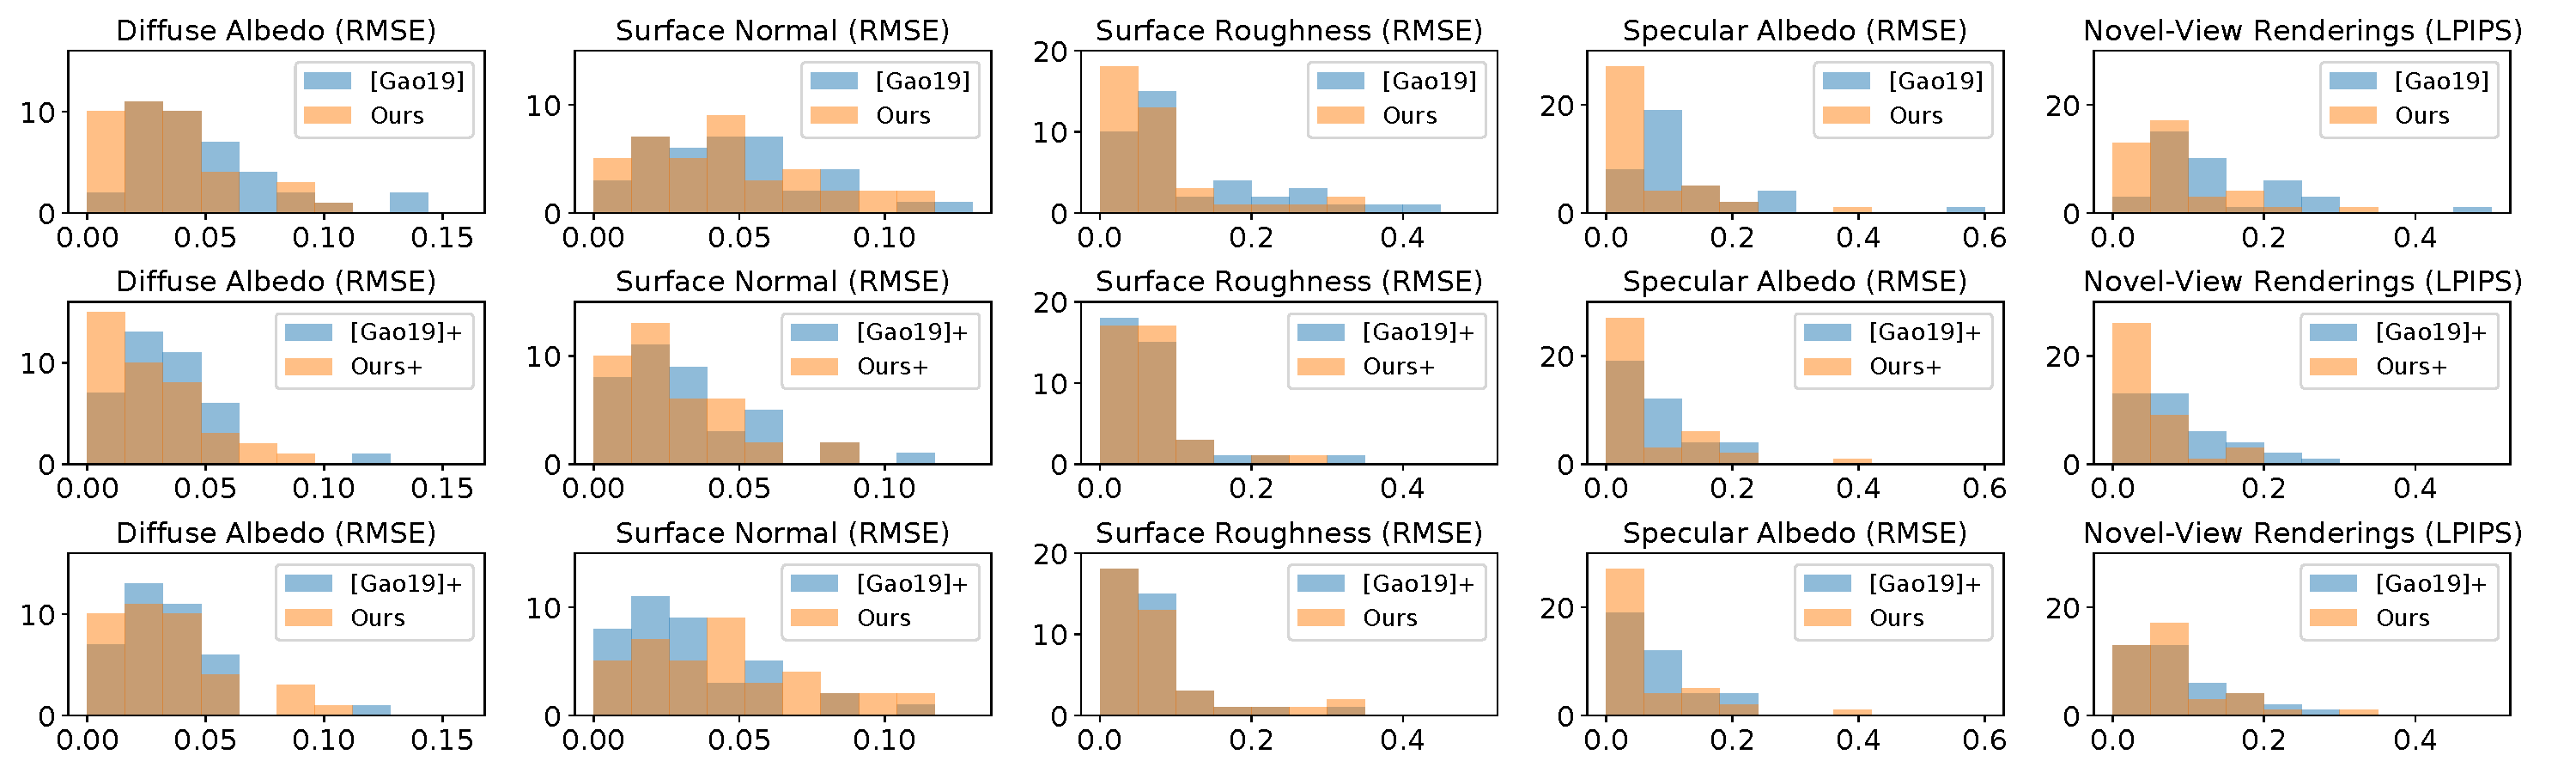
\includegraphics[height=\resLen]{svbrdf/results/rmse/hist_fake.pdf} &
		\includegraphics[height=\resLen]{svbrdf/results/rmse/hist_real.pdf}\\[-4pt]
	\end{tabular}
	\caption[Performance statistics]{\label{fig:svbrdf:rmse}
		\footnotesize \textbf{Performance statistics} of Gao \cite{gao2019deep} and our method.
		For each technique, we compute (i) the Learned Perceptual Image Patch Similarity (LPIPS) metric between renderings of the output SVBRDF maps and the reference images for 40 \emph{real} and 30 \emph{synthetic} examples; and (ii) the root-measure-square error (RMSE) of the inferred maps for the \emph{synthetic} examples.
		For both metrics, a lower score indicates a better accuracy.
		Using identical initializations, our technique (``Ours'' and ``Ours+'') outperforms Gao's (``[Gao19]'' and ``[Gao19]+'') consistently for both real and synthetic examples, as demonstrated in the top and the middle row.
		Furthermore, our technique with constant initializations (``Ours'') has a similar performance with Gao's method initialized using Deschaintre's \cite{deschaintre2019flexible} direct predictions (``[Gao19]+'') on the synthetic examples and outperforms the latter on the real examples, as shown on the bottom.
	}
\end{figure}

%
\subsection{Comparison with prior work on real data}
\label{ssec:real}
%
Here we compare our method and Gao et al. \shortcite{Gao2019}. For more results and comparisons, including with Deschaintre et al. \shortcite{Deschaintre2019}, and including with and without initialization for ours and Gao's method, please refer to supplemental materials.
%
We show 10 real examples from our cell phone capture pipeline in Figure \ref{fig:real}. Note that Gao's method is significantly dependent on initialization, while the same is not true for our method. Therefore, in this figure, we show Gao's result \emph{with initialization} by Deschaintre et al. \shortcite{Deschaintre2019}, while our result is shown \emph{without initialization}.
%
Furthermore, note that we are initializing Gao's method with the 2019 multi-input method by Deschaintre, which is a better initialization than the 2018 single-input method. Thus the baseline we are comparing against is, strictly speaking, even higher than what is published in Gao et al., and combines the two best methods published at this time.
%
Generally, we find that our method produces cleaner maps and is less prone to overfitting (burn-in) than Gao's, while producing more accurate re-renderings under original and novel lighting. Table~\ref{tab:accuracy} shows a quantitative evaluation of the re-rendering quality on novel lighting. As these novel views would be hard to match pixel-wise using any method, as they have never been observed, we use a perceptual method, specifically the Learned Perceptual Image Patch Similarity (LPIPS) metric \cite{LPIPS} (lower is better). Note that our method (without initialization by Deschaintre's method) produces better scores for novel views than Gao's method (with initialization) for most images; even in the case where our LPIPS score is worse, our maps still look more plausible overall.
%
We also report quantitative evaluations (histograms) for our entire set of results (see Figure \ref{fig:rmse}). For synthetic data, we compare the RMSE of all predicted maps (diffuse albedo, normal, roughness, specular albedo), as we do know the ground truth for them. For both synthetic and real data, we compare the LPIPS scores on novel lighting. We use a + sign to indicate initialization by Deschaintre et al. In the top row, we compare both methods without initialization by Deschaintre's method, while in the middle row, both methods are initialized, and in the bottom row, we compare our method without initialization to Gao's with initialization. Generally, we find that if both methods are initialized the same way, our method outperforms Gao's. Even in the last row, our performance is comparable on synthetic data (worse on normal map and better on diffuse/specular maps) and still better on real data overall.
%
\begin{table}[h]
    \centering
    \addtolength{\tabcolsep}{2pt}
    \caption[Accuracy of the novel-view renderings]{\label{tab:svbrdf:accuracy}
    	\textbf{Accuracy of the novel-view renderings} shown in Figure \ref{fig:svbrdf:real} measured using the Learned Perceptual Image Patch Similarity (LPIPS) metric where our method produces better predictions than Gao's \cite{Gao2019} in most cases.
    }
    \begin{tabular}{rcc@{\hspace{2\tabcolsep}}rcc}
        Material & Ours & [Gao19]+ & Material & Ours & [Gao19]+\\
        \hline
        \textit{wall-plaster-white} & \textbf{0.071} & 0.132 & \textit{plastic-red-carton} & \textbf{0.095} & 0.166 \\
        \textit{leather-blue} & \textbf{0.146} & 0.356 & \textit{bathroomtile2} & \textbf{0.225} & 0.231 \\
        \textit{wood-walnut} & \textbf{0.226} & 0.252 & \textit{wood-tile} & 0.202 & \textbf{0.192} \\
        \textit{book1} & \textbf{0.147} & 0.318 & \textit{book2} & \textbf{0.042} & 0.122 \\
        \textit{giftbag1} & \textbf{0.183} & 0.218 & \textit{cards-red} & \textbf{0.059} & 0.092 \\
    \end{tabular}
\end{table}

%
\paragraph{Note about Deschaintre et al.} We find that the results from \cite{Deschaintre2019} have much less accurate re-rendering than either ours or Gao's method, as they are not doing any optimization to precisely fit the target images. The mismatches we observe are definitely not due to simple scaling or gamma correction issues, as that would be consistent across examples; rather, we find that the method performs much better on synthetic examples that match the visual style of its training set. On the other hand, their method is fast and results tend to be clean and artifact-free, so they are very suitable for initialization of optimization methods.
%
\subsection{Additional comparisons}
%
\begin{figure}[h!]
	\centering
	\setlength{\resLen}{0.5in}
	\setlength{\raiseLen}{0.2in}
	\addtolength{\tabcolsep}{-5pt}
	\scriptsize
	\begin{tabular}{lcccc@{\hspace{2\tabcolsep}}ccc}
		& & SVBRDF maps &
		\multicolumn{2}{c}{Novel views}
		& SVBRDF maps & 
		\multicolumn{2}{c}{Novel views}
		\\
		& \raisebox{\raiseLen}{\rotatebox[origin=c]{90}{GT}} &
		\includegraphics[height=\resLen]{svbrdf/results/init/fake_030/ref/tex.jpg} &
		\includegraphics[height=\resLen]{svbrdf/results/init/fake_030/ref/07.jpg} &
		\includegraphics[height=\resLen]{svbrdf/results/init/fake_030/ref/08.jpg} &
		 &
		\includegraphics[height=\resLen]{svbrdf/results/init/real_other-bamboo-veawe/ref/07.jpg} &
		\includegraphics[height=\resLen]{svbrdf/results/init/real_other-bamboo-veawe/ref/08.jpg}
		\\
		& \raisebox{\raiseLen}{\rotatebox[origin=c]{90}{[Des.]}} &
		\includegraphics[height=\resLen]{svbrdf/results/init/fake_030/egsr/tex.jpg} &
		\includegraphics[height=\resLen]{svbrdf/results/init/fake_030/egsr/07.jpg} &
		\includegraphics[height=\resLen]{svbrdf/results/init/fake_030/egsr/08.jpg} &
		\includegraphics[height=\resLen]{svbrdf/results/init/real_other-bamboo-veawe/egsr/tex.jpg} &
		\includegraphics[height=\resLen]{svbrdf/results/init/real_other-bamboo-veawe/egsr/07.jpg} &
		\includegraphics[height=\resLen]{svbrdf/results/init/real_other-bamboo-veawe/egsr/08.jpg}
		\\[1pt]
		\hline\\[-5pt]
		\multirow{2}{*}[\raiseLen]{\rotatebox[origin=c]{90}{Constant init.}} &
		\raisebox{\raiseLen}{\rotatebox[origin=c]{90}{Ours}} &
		\includegraphics[height=\resLen]{svbrdf/results/init/fake_030/ours+/tex.jpg} &
		\includegraphics[height=\resLen]{svbrdf/results/init/fake_030/ours+/07.jpg} &
		\includegraphics[height=\resLen]{svbrdf/results/init/fake_030/ours+/08.jpg} &
		\includegraphics[height=\resLen]{svbrdf/results/init/real_other-bamboo-veawe/ours+/tex.jpg} &
		\includegraphics[height=\resLen]{svbrdf/results/init/real_other-bamboo-veawe/ours+/07.jpg} &
		\includegraphics[height=\resLen]{svbrdf/results/init/real_other-bamboo-veawe/ours+/08.jpg}
		\\
		& \raisebox{\raiseLen}{\rotatebox[origin=c]{90}{[Gao19]}} &
		\includegraphics[height=\resLen]{svbrdf/results/init/fake_030/msra+/tex.jpg} &
		\includegraphics[height=\resLen]{svbrdf/results/init/fake_030/msra+/07.jpg} &
		\includegraphics[height=\resLen]{svbrdf/results/init/fake_030/msra+/08.jpg} &
		\includegraphics[height=\resLen]{svbrdf/results/init/real_other-bamboo-veawe/msra+/tex.jpg} &
		\includegraphics[height=\resLen]{svbrdf/results/init/real_other-bamboo-veawe/msra+/07.jpg} &
		\includegraphics[height=\resLen]{svbrdf/results/init/real_other-bamboo-veawe/msra+/08.jpg}
		\\[1pt]
		\hline\\[-5pt]
		\multirow{2}{*}[1.5\raiseLen]{\rotatebox{90}{[Des]-based init.}} &
		\raisebox{\raiseLen}{\rotatebox[origin=c]{90}{\footnotesize{Ours+}}} &
		\includegraphics[height=\resLen]{svbrdf/results/init/fake_030/ours+_egsr/tex.jpg} &
		\includegraphics[height=\resLen]{svbrdf/results/init/fake_030/ours+_egsr/07.jpg} &
		\includegraphics[height=\resLen]{svbrdf/results/init/fake_030/ours+_egsr/08.jpg} &
		\includegraphics[height=\resLen]{svbrdf/results/init/real_other-bamboo-veawe/ours+_egsr/tex.jpg} &
		\includegraphics[height=\resLen]{svbrdf/results/init/real_other-bamboo-veawe/ours+_egsr/07.jpg} &
		\includegraphics[height=\resLen]{svbrdf/results/init/real_other-bamboo-veawe/ours+_egsr/08.jpg}
		\\
		& \raisebox{\raiseLen}{\rotatebox[origin=c]{90}{[Gao19]+}} &
		\includegraphics[height=\resLen]{svbrdf/results/init/fake_030/msra+_egsr/tex.jpg} &
		\includegraphics[height=\resLen]{svbrdf/results/init/fake_030/msra+_egsr/07.jpg} &
		\includegraphics[height=\resLen]{svbrdf/results/init/fake_030/msra+_egsr/08.jpg} &
		\includegraphics[height=\resLen]{svbrdf/results/init/real_other-bamboo-veawe/msra+_egsr/tex.jpg} &
		\includegraphics[height=\resLen]{svbrdf/results/init/real_other-bamboo-veawe/msra+_egsr/07.jpg} &
		\includegraphics[height=\resLen]{svbrdf/results/init/real_other-bamboo-veawe/msra+_egsr/08.jpg}
		\\
	\end{tabular}
	\caption[SVBRDF results with different initialization]{\label{fig:svbrdf:diff_init}
		\small \textbf{SVBRDF results with different initialization} Unlike Gao's method, ours is less strongly dependent on a good initialization from Deschaintre's method \cite{Deschaintre2019}. In most of cases, starting from simple texture maps (given by our constant initializations) is already good enough to converge to a clean solution. We show all combinations (with and without good initializations) for both methods, for one synthetic and one real example, where techniques initialized with [Deschaintre] are denoted with the suffix ``+'' (i.e., ``Ours+'' and ``[Gao19]+''). Note the failure of Gao's method without good initializations (i.e., ``Gao19'').}
\end{figure}


%
\paragraph{Optimization with different initializations.}
In Figure \ref{fig:result_init}, we compare our method to Gao's with and without initialization by Deschaintre's method in all 4 combinations, on a synthetic and a real example. This shows that Gao's method more significantly dependent on good initialization that ours (even though our method can still occasionally benefit).
%
\begin{figure}[h!]
    \centering
    \setlength{\resLen}{0.5in}
    \setlength{\raiseLen}{0.2in}
    \addtolength{\tabcolsep}{-5pt}
    \scriptsize
    \begin{tabular}{rrlrcc@{\hspace{2\tabcolsep}}lrcc}
    	&
        & \multicolumn{2}{c}{SVBRDF maps} & \multicolumn{2}{c}{Novel views}
        & \multicolumn{2}{c}{SVBRDF maps} & \multicolumn{2}{c}{Novel views}
        \\[2pt]
        & &
        & \raisebox{\raiseLen}{\rotatebox[origin=c]{90}{GT}} &
        \includegraphics[height=\resLen]{svbrdf/results/refine/real_wood-knotty/ref/rendered_nov_1.jpg} &
        \includegraphics[height=\resLen]{svbrdf/results/refine/real_wood-knotty/ref/rendered_nov_2.jpg} &
        & \raisebox{\raiseLen}{\rotatebox[origin=c]{90}{GT}} &
        \includegraphics[height=\resLen]{svbrdf/results/refine/real_cards-blue/ref/rendered_nov_1.jpg} &
        \includegraphics[height=\resLen]{svbrdf/results/refine/real_cards-blue/ref/rendered_nov_2.jpg}
        \\[-1pt]
        & &
        \textit{~~wood-knotty} & &
        \includegraphics[height=0.5\resLen]{svbrdf/results/refine/real_wood-knotty/ref/rendered_nov_1_zoom.jpg} &
        \includegraphics[height=0.5\resLen]{svbrdf/results/refine/real_wood-knotty/ref/rendered_nov_2_zoom.jpg} &
        \textit{~~cards-blue} & &
        \includegraphics[height=0.5\resLen]{svbrdf/results/refine/real_cards-blue/ref/rendered_nov_1_zoom.jpg} &
        \includegraphics[height=0.5\resLen]{svbrdf/results/refine/real_cards-blue/ref/rendered_nov_2_zoom.jpg}
        \\[1pt]
        \multirow{4}{*}[0.5\raiseLen]{\rotatebox[origin=c]{90}{No refinement}} &
        \raisebox{\raiseLen}{\rotatebox[origin=c]{90}{Ours}} &
        \multicolumn{2}{c}{\includegraphics[height=\resLen]{svbrdf/results/refine/real_wood-knotty/ours/tex.jpg}} &
        \includegraphics[height=\resLen]{svbrdf/results/refine/real_wood-knotty/ours/rendered_nov_1.jpg} &
        \includegraphics[height=\resLen]{svbrdf/results/refine/real_wood-knotty/ours/rendered_nov_2.jpg} &
        \multicolumn{2}{c}{\includegraphics[height=\resLen]{svbrdf/results/refine/real_cards-blue/ours/tex.jpg}} &
        \includegraphics[height=\resLen]{svbrdf/results/refine/real_cards-blue/ours/rendered_nov_1.jpg} &
        \includegraphics[height=\resLen]{svbrdf/results/refine/real_cards-blue/ours/rendered_nov_2.jpg}
        \\[-1pt]
        & &
        \multicolumn{2}{c}{\includegraphics[height=0.5\resLen]{svbrdf/results/refine/real_wood-knotty/ours/tex_zoom.jpg}} &
        \includegraphics[height=0.5\resLen]{svbrdf/results/refine/real_wood-knotty/ours/rendered_nov_1_zoom.jpg} &
        \includegraphics[height=0.5\resLen]{svbrdf/results/refine/real_wood-knotty/ours/rendered_nov_2_zoom.jpg} &
        \multicolumn{2}{c}{\includegraphics[height=0.5\resLen]{svbrdf/results/refine/real_cards-blue/ours/tex_zoom.jpg}} &
        \includegraphics[height=0.5\resLen]{svbrdf/results/refine/real_cards-blue/ours/rendered_nov_1_zoom.jpg} &
        \includegraphics[height=0.5\resLen]{svbrdf/results/refine/real_cards-blue/ours/rendered_nov_2_zoom.jpg}
        \\[1pt]
        & \raisebox{\raiseLen}{\rotatebox[origin=c]{90}{[Gao19]+}} &
        \multicolumn{2}{c}{\includegraphics[height=\resLen]{svbrdf/results/refine/real_wood-knotty/msra_egsr/tex.jpg}} &
        \includegraphics[height=\resLen]{svbrdf/results/refine/real_wood-knotty/msra_egsr/rendered_nov_1.jpg} &
        \includegraphics[height=\resLen]{svbrdf/results/refine/real_wood-knotty/msra_egsr/rendered_nov_2.jpg} &
        \multicolumn{2}{c}{\includegraphics[height=\resLen]{svbrdf/results/refine/real_cards-blue/msra_egsr/tex.jpg}} &
        \includegraphics[height=\resLen]{svbrdf/results/refine/real_cards-blue/msra_egsr/rendered_nov_1.jpg} &
        \includegraphics[height=\resLen]{svbrdf/results/refine/real_cards-blue/msra_egsr/rendered_nov_2.jpg}
        \\[-1pt]
        & &
        \multicolumn{2}{c}{\includegraphics[height=0.5\resLen]{svbrdf/results/refine/real_wood-knotty/msra_egsr/tex_zoom.jpg}} &
        \includegraphics[height=0.5\resLen]{svbrdf/results/refine/real_wood-knotty/msra_egsr/rendered_nov_1_zoom.jpg} &
        \includegraphics[height=0.5\resLen]{svbrdf/results/refine/real_wood-knotty/msra_egsr/rendered_nov_2_zoom.jpg} &
        \multicolumn{2}{c}{\includegraphics[height=0.5\resLen]{svbrdf/results/refine/real_cards-blue/msra_egsr/tex_zoom.jpg}} &
        \includegraphics[height=0.5\resLen]{svbrdf/results/refine/real_cards-blue/msra_egsr/rendered_nov_1_zoom.jpg} &
        \includegraphics[height=0.5\resLen]{svbrdf/results/refine/real_cards-blue/msra_egsr/rendered_nov_2_zoom.jpg}
        \\[1pt]
        \hline\\[-6pt]
        \multirow{4}{*}[0.5\raiseLen]{\rotatebox[origin=c]{90}{With refinement}} &
        \raisebox{\raiseLen}{\rotatebox[origin=c]{90}{Ours}} &
		\multicolumn{2}{c}{\includegraphics[height=\resLen]{svbrdf/results/refine/real_wood-knotty/ours+/tex.jpg}} &
		\includegraphics[height=\resLen]{svbrdf/results/refine/real_wood-knotty/ours+/rendered_nov_1.jpg} &
		\includegraphics[height=\resLen]{svbrdf/results/refine/real_wood-knotty/ours+/rendered_nov_2.jpg} &
		\multicolumn{2}{c}{\includegraphics[height=\resLen]{svbrdf/results/refine/real_cards-blue/ours+/tex.jpg}} &
		\includegraphics[height=\resLen]{svbrdf/results/refine/real_cards-blue/ours+/rendered_nov_1.jpg} &
		\includegraphics[height=\resLen]{svbrdf/results/refine/real_cards-blue/ours+/rendered_nov_2.jpg}
		\\[-1pt]
		& &
		\multicolumn{2}{c}{\includegraphics[height=0.5\resLen]{svbrdf/results/refine/real_wood-knotty/ours+/tex_zoom.jpg}} &
		\includegraphics[height=0.5\resLen]{svbrdf/results/refine/real_wood-knotty/ours+/rendered_nov_1_zoom.jpg} &
		\includegraphics[height=0.5\resLen]{svbrdf/results/refine/real_wood-knotty/ours+/rendered_nov_2_zoom.jpg} &
		\multicolumn{2}{c}{\includegraphics[height=0.5\resLen]{svbrdf/results/refine/real_cards-blue/ours+/tex_zoom.jpg}} &
		\includegraphics[height=0.5\resLen]{svbrdf/results/refine/real_cards-blue/ours+/rendered_nov_1_zoom.jpg} &
		\includegraphics[height=0.5\resLen]{svbrdf/results/refine/real_cards-blue/ours+/rendered_nov_2_zoom.jpg}
		\\[1pt]
        & \raisebox{\raiseLen}{\rotatebox[origin=c]{90}{[Gao19]+}} &
        \multicolumn{2}{c}{\includegraphics[height=\resLen]{svbrdf/results/refine/real_wood-knotty/msra+_egsr/tex.jpg}} &
        \includegraphics[height=\resLen]{svbrdf/results/refine/real_wood-knotty/msra+_egsr/rendered_nov_1.jpg} &
        \includegraphics[height=\resLen]{svbrdf/results/refine/real_wood-knotty/msra+_egsr/rendered_nov_2.jpg} &
        \multicolumn{2}{c}{\includegraphics[height=\resLen]{svbrdf/results/refine/real_cards-blue/msra+_egsr/tex.jpg}} &
        \includegraphics[height=\resLen]{svbrdf/results/refine/real_cards-blue/msra+_egsr/rendered_nov_1.jpg} &
        \includegraphics[height=\resLen]{svbrdf/results/refine/real_cards-blue/msra+_egsr/rendered_nov_2.jpg}
        \\[-1pt]
        & &
        \multicolumn{2}{c}{\includegraphics[height=0.5\resLen]{svbrdf/results/refine/real_wood-knotty/msra+_egsr/tex_zoom.jpg}} &
        \includegraphics[height=0.5\resLen]{svbrdf/results/refine/real_wood-knotty/msra+_egsr/rendered_nov_1_zoom.jpg} &
        \includegraphics[height=0.5\resLen]{svbrdf/results/refine/real_wood-knotty/msra+_egsr/rendered_nov_2_zoom.jpg} &
        \multicolumn{2}{c}{\includegraphics[height=0.5\resLen]{svbrdf/results/refine/real_cards-blue/msra+_egsr/tex_zoom.jpg}} &
        \includegraphics[height=0.5\resLen]{svbrdf/results/refine/real_cards-blue/msra+_egsr/rendered_nov_1_zoom.jpg} &
        \includegraphics[height=0.5\resLen]{svbrdf/results/refine/real_cards-blue/msra+_egsr/rendered_nov_2_zoom.jpg}
    \end{tabular}
    \caption[Per-pixel post-refinement]{\label{fig:svbrdf:refine}
        \small \textbf{Per-pixel post-refinement.} Unlike Gao's method, post-refinement via per-pixel optimization makes less of a difference in our method.
        Without post-refinement, [Gao19]+ (i.e., Gao's method initialized with Deschaintre's \cite{deschaintre2019flexible} direct predictions) usually produces blurry results, as shown in the row marked as ``[Gao19]+ (NR)''.
        Our method, on the contrary, does not rely nearly as heavily on post-refinement: Without it, our results are already quite sharp (see ``Ours (NR)''), thanks to the generative power of our MaterialGAN.
        A zoomed-in version is attached below each SVBRDF map and novel-view image.
    }
\end{figure}

%
\paragraph{Post-refinement.}
In general, the quality of our maps is sufficient after using our MaterialGAN-based optimization. However, Gao's method introduced a post-refinement step, where the maps are further optimized without any latent space, and with at most minor regularization. Therefore, we also implement a similar post-refinement step. However, like good initialization, this post-refinement makes less of a difference in our method, and Gao's method is more dependent on it, as it produces significantly blurry maps without it. This is shown in Figure \ref{fig:refine}; note the difference in sharpness of the maps.
%
\begin{figure}[h]
	\centering
	\setlength{\resLen}{.5in}
	\setlength{\raiseLen}{.2in}
	\addtolength{\tabcolsep}{-5.5pt}
	\scriptsize
	\begin{tabular}{ccccc@{\hspace{4\tabcolsep}}cccc@{\hspace{4\tabcolsep}}cccc}
		\raisebox{.31in}{\rotatebox[origin=c]{90}{GT Novel}} &
		\raisebox{0.1in}{\includegraphics[height=\resLen]{svbrdf/results/multi/fake_010/ref/27.jpg}} &
		\multicolumn{3}{l}{\includegraphics[height=1.7\resLen]{svbrdf/results/multi/fake_010/err.pdf}} &
		\raisebox{0.1in}{\includegraphics[height=\resLen]{svbrdf/results/multi/fake_006/ref/27.jpg}} &
		\multicolumn{3}{l}{\includegraphics[height=1.7\resLen]{svbrdf/results/multi/fake_006/err.pdf}} &
		\raisebox{0.1in}{\includegraphics[height=\resLen]{svbrdf/results/multi/fake_015/ref/27.jpg}} &
		\multicolumn{3}{l}{\includegraphics[height=1.7\resLen]{svbrdf/results/multi/fake_015/err.pdf}}
		\\
		& \textbf{\small N=1} & \textbf{\small 5} & \textbf{\small 9} & \textbf{\small 25}
		& \textbf{\small N=1} & \textbf{\small 5} & \textbf{\small 9} & \textbf{\small 25}
		& \textbf{\small N=1} & \textbf{\small 5} & \textbf{\small 9} & \textbf{\small 25}
		\\
		\raisebox{\raiseLen}{\rotatebox[origin=c]{90}{Ours}} &
		\includegraphics[height=\resLen]{svbrdf/results/multi/fake_010/ours+_1/27.jpg} &
		\includegraphics[height=\resLen]{svbrdf/results/multi/fake_010/ours+_5/27.jpg} &
		\includegraphics[height=\resLen]{svbrdf/results/multi/fake_010/ours+_9/27.jpg} &
		\includegraphics[height=\resLen]{svbrdf/results/multi/fake_010/ours+_25/27.jpg} &
		\includegraphics[height=\resLen]{svbrdf/results/multi/fake_006/ours+_1/27.jpg} &
		\includegraphics[height=\resLen]{svbrdf/results/multi/fake_006/ours+_5/27.jpg} &
		\includegraphics[height=\resLen]{svbrdf/results/multi/fake_006/ours+_9/27.jpg} &
		\includegraphics[height=\resLen]{svbrdf/results/multi/fake_006/ours+_25/27.jpg} &
		\includegraphics[height=\resLen]{svbrdf/results/multi/fake_015/ours+_1/27.jpg} &
		\includegraphics[height=\resLen]{svbrdf/results/multi/fake_015/ours+_5/27.jpg} &
		\includegraphics[height=\resLen]{svbrdf/results/multi/fake_015/ours+_9/27.jpg} &
		\includegraphics[height=\resLen]{svbrdf/results/multi/fake_015/ours+_25/27.jpg}
		\\
		\raisebox{\raiseLen}{\rotatebox[origin=c]{90}{Ours+}} &
		\includegraphics[height=\resLen]{svbrdf/results/multi/fake_010/ours+_egsr_1/27.jpg} &
		\includegraphics[height=\resLen]{svbrdf/results/multi/fake_010/ours+_egsr_5/27.jpg} &
		\includegraphics[height=\resLen]{svbrdf/results/multi/fake_010/ours+_egsr_9/27.jpg} &
		\includegraphics[height=\resLen]{svbrdf/results/multi/fake_010/ours+_egsr_25/27.jpg} &
		\includegraphics[height=\resLen]{svbrdf/results/multi/fake_006/ours+_egsr_1/27.jpg} &
		\includegraphics[height=\resLen]{svbrdf/results/multi/fake_006/ours+_egsr_5/27.jpg} &
		\includegraphics[height=\resLen]{svbrdf/results/multi/fake_006/ours+_egsr_9/27.jpg} &
		\includegraphics[height=\resLen]{svbrdf/results/multi/fake_006/ours+_egsr_25/27.jpg} &
		\includegraphics[height=\resLen]{svbrdf/results/multi/fake_015/ours+_egsr_1/27.jpg} &
		\includegraphics[height=\resLen]{svbrdf/results/multi/fake_015/ours+_egsr_5/27.jpg} &
		\includegraphics[height=\resLen]{svbrdf/results/multi/fake_015/ours+_egsr_9/27.jpg} &
		\includegraphics[height=\resLen]{svbrdf/results/multi/fake_015/ours+_egsr_25/27.jpg}
		\\
		\raisebox{\raiseLen}{\rotatebox[origin=c]{90}{[Gao19]+}} &
		\includegraphics[height=\resLen]{svbrdf/results/multi/fake_010/msra+_1/27.jpg} &
		\includegraphics[height=\resLen]{svbrdf/results/multi/fake_010/msra+_5/27.jpg} &
		\includegraphics[height=\resLen]{svbrdf/results/multi/fake_010/msra+_9/27.jpg} &
		\includegraphics[height=\resLen]{svbrdf/results/multi/fake_010/msra+_25/27.jpg} &
		\includegraphics[height=\resLen]{svbrdf/results/multi/fake_006/msra+_1/27.jpg} &
		\includegraphics[height=\resLen]{svbrdf/results/multi/fake_006/msra+_5/27.jpg} &
		\includegraphics[height=\resLen]{svbrdf/results/multi/fake_006/msra+_9/27.jpg} &
		\includegraphics[height=\resLen]{svbrdf/results/multi/fake_006/msra+_25/27.jpg} &
		\includegraphics[height=\resLen]{svbrdf/results/multi/fake_015/msra+_1/27.jpg} &
		\includegraphics[height=\resLen]{svbrdf/results/multi/fake_015/msra+_5/27.jpg} &
		\includegraphics[height=\resLen]{svbrdf/results/multi/fake_015/msra+_9/27.jpg} &
		\includegraphics[height=\resLen]{svbrdf/results/multi/fake_015/msra+_25/27.jpg}
	\end{tabular}
	\caption[Performance using different numbers of input images (synthetic data)]{\label{fig:svbrdf:multi_fake}
		\small \textbf{Performance using different numbers of input images (synthetic data).}
		The quality of recovered SVBRDF maps, as demonstrated by the plots, generally improves with more input images for both our and Gao's \cite{gao2019deep} methods.
		Our method with constant (Ours) and neural (Ours+) initializations are comparable or better than Gao's  ([Gao19]+) with neural initialization \cite{deschaintre2019flexible} .
		For a highly specular material shown on the right, although the LPIPS metric computed using renderings under 5 novel views of our results is similar to that of Gao's, ours better preserve the specular highlight.
		For each material, all the renderings including the references (GT Novel) are generated using one of the 5 novel views.
	}
\end{figure}
\begin{figure}[h]
	\centering
	\setlength{\resLen}{0.5in}
	\setlength{\raiseLen}{0.23in}
	\addtolength{\tabcolsep}{-5pt}
	\scriptsize
	\begin{tabular}{ccccc@{\hspace{4\tabcolsep}}ccc}
		& & SVBRDF maps &
		\multicolumn{2}{c}{Novel views} &
		SVBRDF maps &
		\multicolumn{2}{c}{Novel views}
		\\
		\multirow{3}{*}[-1\raiseLen]{\rotatebox[origin=c]{90}{Ours}} &
		\raisebox{\raiseLen}{\rotatebox[origin=c]{0}{1}} &
		\includegraphics[height=\resLen]{svbrdf/results/multi_real/real_plastic-red-carton/ours+_1/tex.jpg} &
		\includegraphics[height=\resLen]{svbrdf/results/multi_real/real_plastic-red-carton/ours+_1/07.jpg} &
		\includegraphics[height=\resLen]{svbrdf/results/multi_real/real_plastic-red-carton/ours+_1/08.jpg} &
		\includegraphics[height=\resLen]{svbrdf/results/multi_real/real_cards-red/ours+_1/tex.jpg} &
		\includegraphics[height=\resLen]{svbrdf/results/multi_real/real_cards-red/ours+_1/07.jpg} &
		\includegraphics[height=\resLen]{svbrdf/results/multi_real/real_cards-red/ours+_1/08.jpg}
		\\
		& \raisebox{\raiseLen}{\rotatebox[origin=c]{0}{3}} &
		\includegraphics[height=\resLen]{svbrdf/results/multi_real/real_plastic-red-carton/ours+_3/tex.jpg} &
		\includegraphics[height=\resLen]{svbrdf/results/multi_real/real_plastic-red-carton/ours+_3/07.jpg} &
		\includegraphics[height=\resLen]{svbrdf/results/multi_real/real_plastic-red-carton/ours+_3/08.jpg} &
		\includegraphics[height=\resLen]{svbrdf/results/multi_real/real_cards-red/ours+_3/tex.jpg} &
		\includegraphics[height=\resLen]{svbrdf/results/multi_real/real_cards-red/ours+_3/07.jpg} &
		\includegraphics[height=\resLen]{svbrdf/results/multi_real/real_cards-red/ours+_3/08.jpg}
		\\
		& \raisebox{\raiseLen}{\rotatebox[origin=c]{0}{7}} &
		\includegraphics[height=\resLen]{svbrdf/results/multi_real/real_plastic-red-carton/ours+_7/tex.jpg} &
		\includegraphics[height=\resLen]{svbrdf/results/multi_real/real_plastic-red-carton/ours+_7/07.jpg} &
		\includegraphics[height=\resLen]{svbrdf/results/multi_real/real_plastic-red-carton/ours+_7/08.jpg} &
		\includegraphics[height=\resLen]{svbrdf/results/multi_real/real_cards-red/ours+_7/tex.jpg} &
		\includegraphics[height=\resLen]{svbrdf/results/multi_real/real_cards-red/ours+_7/07.jpg} &
		\includegraphics[height=\resLen]{svbrdf/results/multi_real/real_cards-red/ours+_7/08.jpg}
		\\[1pt]
		\hline \\[-6pt]
		\multirow{3}{*}[-1\raiseLen]{\rotatebox[origin=c]{90}{Ours+}} &
		\raisebox{\raiseLen}{\rotatebox[origin=c]{0}{1}} &
		\includegraphics[height=\resLen]{svbrdf/results/multi_real/real_plastic-red-carton/ours+_egsr_1/tex.jpg} &
		\includegraphics[height=\resLen]{svbrdf/results/multi_real/real_plastic-red-carton/ours+_egsr_1/07.jpg} &
		\includegraphics[height=\resLen]{svbrdf/results/multi_real/real_plastic-red-carton/ours+_egsr_1/08.jpg} &
		\includegraphics[height=\resLen]{svbrdf/results/multi_real/real_cards-red/ours+_egsr_1/tex.jpg} &
		\includegraphics[height=\resLen]{svbrdf/results/multi_real/real_cards-red/ours+_egsr_1/07.jpg} &
		\includegraphics[height=\resLen]{svbrdf/results/multi_real/real_cards-red/ours+_egsr_1/08.jpg}
		\\
		& \raisebox{\raiseLen}{\rotatebox[origin=c]{0}{3}} &
		\includegraphics[height=\resLen]{svbrdf/results/multi_real/real_plastic-red-carton/ours+_egsr_3/tex.jpg} &
		\includegraphics[height=\resLen]{svbrdf/results/multi_real/real_plastic-red-carton/ours+_egsr_3/07.jpg} &
		\includegraphics[height=\resLen]{svbrdf/results/multi_real/real_plastic-red-carton/ours+_egsr_3/08.jpg} &
		\includegraphics[height=\resLen]{svbrdf/results/multi_real/real_cards-red/ours+_egsr_3/tex.jpg} &
		\includegraphics[height=\resLen]{svbrdf/results/multi_real/real_cards-red/ours+_egsr_3/07.jpg} &
		\includegraphics[height=\resLen]{svbrdf/results/multi_real/real_cards-red/ours+_egsr_3/08.jpg}
		\\
		& \raisebox{\raiseLen}{\rotatebox[origin=c]{0}{7}} &
		\includegraphics[height=\resLen]{svbrdf/results/multi_real/real_plastic-red-carton/ours+_egsr_7/tex.jpg} &
		\includegraphics[height=\resLen]{svbrdf/results/multi_real/real_plastic-red-carton/ours+_egsr_7/07.jpg} &
		\includegraphics[height=\resLen]{svbrdf/results/multi_real/real_plastic-red-carton/ours+_egsr_7/08.jpg} &
		\includegraphics[height=\resLen]{svbrdf/results/multi_real/real_cards-red/ours+_egsr_7/tex.jpg} &
		\includegraphics[height=\resLen]{svbrdf/results/multi_real/real_cards-red/ours+_egsr_7/07.jpg} &
		\includegraphics[height=\resLen]{svbrdf/results/multi_real/real_cards-red/ours+_egsr_7/08.jpg}
		\\[1pt]
		\hline\\[-6pt]
		\multirow{3}{*}[-1\raiseLen]{\rotatebox[origin=c]{90}{[Gao19]+}} &
		\raisebox{\raiseLen}{\rotatebox[origin=c]{0}{1}} &
		\includegraphics[height=\resLen]{svbrdf/results/multi_real/real_plastic-red-carton/msra+_egsr_1/tex.jpg} &
		\includegraphics[height=\resLen]{svbrdf/results/multi_real/real_plastic-red-carton/msra+_egsr_1/07.jpg} &
		\includegraphics[height=\resLen]{svbrdf/results/multi_real/real_plastic-red-carton/msra+_egsr_1/08.jpg} &
		\includegraphics[height=\resLen]{svbrdf/results/multi_real/real_cards-red/msra+_egsr_1/tex.jpg} &
		\includegraphics[height=\resLen]{svbrdf/results/multi_real/real_cards-red/msra+_egsr_1/07.jpg} &
		\includegraphics[height=\resLen]{svbrdf/results/multi_real/real_cards-red/msra+_egsr_1/08.jpg}
		\\
		& \raisebox{\raiseLen}{\rotatebox[origin=c]{0}{3}} &
		\includegraphics[height=\resLen]{svbrdf/results/multi_real/real_plastic-red-carton/msra+_egsr_3/tex.jpg} &
		\includegraphics[height=\resLen]{svbrdf/results/multi_real/real_plastic-red-carton/msra+_egsr_3/07.jpg} &
		\includegraphics[height=\resLen]{svbrdf/results/multi_real/real_plastic-red-carton/msra+_egsr_3/08.jpg} &
		\includegraphics[height=\resLen]{svbrdf/results/multi_real/real_cards-red/msra+_egsr_3/tex.jpg} &
		\includegraphics[height=\resLen]{svbrdf/results/multi_real/real_cards-red/msra+_egsr_3/07.jpg} &
		\includegraphics[height=\resLen]{svbrdf/results/multi_real/real_cards-red/msra+_egsr_3/08.jpg}
		\\
		& \raisebox{\raiseLen}{\rotatebox[origin=c]{0}{7}} &
		\includegraphics[height=\resLen]{svbrdf/results/multi_real/real_plastic-red-carton/msra+_egsr_7/tex.jpg} &
		\includegraphics[height=\resLen]{svbrdf/results/multi_real/real_plastic-red-carton/msra+_egsr_7/07.jpg} &
		\includegraphics[height=\resLen]{svbrdf/results/multi_real/real_plastic-red-carton/msra+_egsr_7/08.jpg} &
		\includegraphics[height=\resLen]{svbrdf/results/multi_real/real_cards-red/msra+_egsr_7/tex.jpg} &
		\includegraphics[height=\resLen]{svbrdf/results/multi_real/real_cards-red/msra+_egsr_7/07.jpg} &
		\includegraphics[height=\resLen]{svbrdf/results/multi_real/real_cards-red/msra+_egsr_7/08.jpg}
	\end{tabular}
	\caption[Performance using different numbers of input images (real data)]{\label{fig:svbrdf:multi_real}
		\small \textbf{Performance using different numbers of input images (real data).}
		The quality of SVBRDF maps recovered by our method generally improves with more input images under both constant initialization (see ``Ours'') and Deschaintre \cite{Deschaintre2019} initialization (see ``Ours+'').
	}
\end{figure}
%
\paragraph{Optimization with different numbers of input images.} While most of our results are shown with 7 inputs, using two additional inputs for novel lighting evaluation, our method does work with various numbers of input images. We show 3 synthetic examples in Figure~\ref{fig:results_multi_inputs2}, with different numbers of inputs from 1 to 25. All the three examples are the same as used in Gao's work. The errors of both reconstructed SVBRDF maps and novel-view renderings generally decrease with more input images, as is expected for an inverse-rendering method. In Figure~\ref{fig:results_multi_inputs}, we compare real capture results with 1, 3, and 7 inputs, with and without initialization by Deschaintre's method, and also include Gao's results for 3 and 7 inputs (with initialization). Our result remains plausible with 3 inputs, though artifacts do get reduced with more inputs. For all numbers of inputs, our result (with or without initialization) tends to be cleaner than Gao's.
%
\paragraph{Editing operations.} An additional advantage of the StyleGAN-based latent space is the ability to achieve semantically meaningful operations such as morphing, by interpolating two or more parent latent codes to create a hybrid offspring material. Morphing in latent space often preserves semantic features qualitatively better than naive interpolation in pixel space. Figure~\ref{fig:interp}~\revision{and the supplemental video show} morphing of a few real materials using linear interpolation in latent space, compared to the corresponding naive interpolation (linear in pixel space).
%
\begin{figure}[!ht]
	\centering
	\setlength{\resLen}{3.2in}
	\addtolength{\tabcolsep}{-3.5pt}
	\begin{tabular}{cc}
		GAN-based interpolation of SVBRDF maps & Linear interpolation of SVBRDF maps\\
		\includegraphics[width=\resLen]{svbrdf/results/morph/1_gan.jpg} &
		\includegraphics[width=\resLen]{svbrdf/results/morph/1_naive.jpg}\\
		\includegraphics[width=\resLen]{svbrdf/results/morph/2_gan.jpg} &
		\includegraphics[width=\resLen]{svbrdf/results/morph/2_naive.jpg}\\
		\includegraphics[width=\resLen]{svbrdf/results/morph/3_gan.jpg} &
		\includegraphics[width=\resLen]{svbrdf/results/morph/3_naive.jpg}
	\end{tabular}
	\caption[Material interpolation]{\label{fig:svbrdf:morph_real}
		\textbf{Material interpolation.} Renderings of interpolations between two SVBRDFs recovered from real images using our method. Results on the left and right columns are obtained, respectively, using our GAN latent space and na\"ive linear interpolation.
	}
\end{figure}

%